% This is samplepaper.tex, a sample chapter demonstrating the
% LLNCS macro package for Springer Computer Science proceedings;
% Version 2.20 of 2017/10/04
%
\documentclass[runningheads]{llncs2e/llncs}
%
\usepackage{xspace}
\usepackage[dvipsnames]{xcolor}
\usepackage{amsmath}
\usepackage{afterpage}  
\usepackage{figlatex,wrapfig}
\usepackage[dvipsnames]{xcolor}
\usepackage{listings,amssymb,mathtools}
\usepackage{mathrsfs}
\usepackage{array,multirow}
\usepackage{caption}
%\usepackage{textcomp}
\usepackage{algorithm}
\usepackage[noend]{algpseudocode}
\usepackage{framed,enumitem}

% for colours
\usepackage{xspace}
\usepackage[colorlinks]{hyperref}
\hypersetup{
	colorlinks = true,
	citecolor = {violet},
	linkcolor = {blue},
	urlcolor  = {blue}
}

% for arrow diagrams
\usepackage{amsmath}
\usepackage{amssymb}
\usepackage{smartdiagram}
\usepackage{tikz}
\usetikzlibrary{arrows,positioning}

%\usepackage[parfill]{parskip}

% for bib handline
%\usepackage[numbers]{natbib}
%\usepackage{url}

% implies and iff arrows
\renewcommand{\iff}{\xspace\Leftrightarrow\xspace}
\renewcommand{\implies}{\xspace\Rightarrow\xspace}
\newcommand{\onlyif}{\xspace\Leftarrow\xspace}

% commonly used abbreviations and expressions
\renewcommand{\th}{^{th}\xspace} % superscript th for numbers eg i^{th}
\newcommand{\definedas}{\triangleq\xspace}
\newcommand{\ie}{{\em i.e.}\xspace}
\newcommand{\st}{\ \mbox{s.t.}\ }
\newcommand{\viz}{\textit{viz}.\@\xspace}
\newcommand{\wrt}{\textit{wrt}\xspace}
\newcommand{\wkt}{we know that,\xspace}
\newcommand{\aka}{a.k.a\xspace}
\newcommand{\sota}{state-of-the-art\xspace}
\newcommand{\Sota}{State-of-the-art\xspace}

% common operators
\renewcommand{\^}{\xspace\wedge\xspace}
\renewcommand{\v}{\xspace\vee\xspace}
\newcommand{\xor}{\xspace\veebar\xspace}
\renewcommand{\|}{\ |\ }
\newcommand{\intersection}{\xspace\cap\xspace}
\newcommand{\union}{\xspace\cup\xspace}
\newcommand{\intersectioneq}{\xspace\cap=\xspace}
\newcommand{\unioneq}{\ {\cup}{=}\ }
\newcommand{\nin}{\not\in\xspace}

% highlighted hyperlinks
\newcommand{\hl}[1]{{\textcolor{darkgray}{\texttt{(#1)}}}\xspace} % hyperlink target
\newcommand{\hlref}[1]{\hyperlink{#1}{\textcolor{Sepia}{\small \texttt{(#1)}}}}
\newcommand{\tab}{\quad\quad}

%%%%%%%%%%%%%%%%%%%%%%%%% Document Specific %%%%%%%%%%%%%%%%%%%%%%

% names
\newcommand{\ourtechnique}{\textcolor{RubineRed}{\texttt{FenSyn}}\xspace}
\newcommand{\ourtool}{\ourtechnique{-}tool\xspace}
\newcommand{\cc}{\textit{C11}\xspace}

% sets and entitites
\newcommand{\program}{$P$\xspace} %input program
\newcommand{\programhat}{$\widehat{P}$\xspace} %transformed/fixed program
\newcommand{\fixed}[1]{\widehat{#1}\xspace}
\newcommand{\threads}{\mathcal{T}\xspace}
\newcommand{\states}{\Sigma\xspace}
\newcommand{\moset}{\mathcal{M}\xspace}
\newcommand{\actions}{\mathcal{A}\xspace}
\newcommand{\objects}{\mathcal{O}\xspace}
\newcommand{\s}[1]{s_{[#1]}\xspace} % state reached after exploring sequence #1
% events' sets aux
\newcommand{\wt}[1]{{\mathbb{W}#1}}
\newcommand{\md}[1]{{\mathbb{M}#1}}
\newcommand{\rd}[1]{{\mathbb{R}#1}}
\newcommand{\fn}[1]{{\mathbb{F}#1}}
% events' sets
\newcommand{\events}{\mathcal{E}\xspace}
\newcommand{\writes}{\events^\wt{}\xspace}
\newcommand{\reads}{\events^\rd{}\xspace}
\newcommand{\fences}{\events^\fn{}\xspace}
\newcommand{\ordevents}[1]{\events^{(#1)}\xspace}
\newcommand{\ordwrites}[1]{\events^\wt{(#1)}\xspace}
\newcommand{\ordreads}[1]{\events^\rd{(#1)}\xspace}
\newcommand{\ordfences}[1]{\events^\fn{(#1)}\xspace}


% memory orders
\newcommand{\mosc}{\texttt{seq\_cst}\xspace}
\newcommand{\moar}{\texttt{acq\_rel}\xspace}
\newcommand{\morel}{\texttt{release}\xspace}
\newcommand{\moacq}{\texttt{acquire}\xspace}
\newcommand{\mocon}{\texttt{consume}\xspace}
\newcommand{\morlx}{\texttt{relaxed}\xspace}

% operators
\newcommand{\molt}{{\sqsubset}\xspace}
\newcommand{\mole}{{\sqsubseteq}\xspace}
\newcommand{\mogt}{{\sqsupset}\xspace}
\newcommand{\moge}{{\sqsupseteq}\xspace}

% relations
\newcommand{\reln}[4]{#3 {\rightarrow^{#1}_{#2}} #4\xspace} % any relation specified as #1
\newcommand{\nreln}[4]{#3 \nrightarrow^{#1}_{#2} #4\xspace} % not of any relation specified as #1

% relation with events
\newcommand{\seqb}[3]{\reln{\textbf{\textcolor{CarnationPink}{sb}}}{#1}{#2}{#3}\xspace}
\newcommand{\rf}[3]{\reln{\textbf{\textcolor{PineGreen}{rf}}}{#1}{#2}{#3}\xspace} 
\newcommand{\dob}[3]{\reln{\textbf{\textcolor{Mulberry}{dob}}}{#1}{#2}{#3}\xspace}
\newcommand{\sw}[3]{\reln{\textbf{\textcolor{Magenta}{sw}}}{#1}{#2}{#3}\xspace}
\newcommand{\ithb}[3]{\reln{\textbf{\textcolor{NavyBlue}{ithb}}}{#1}{#2}{#3}\xspace}
\newcommand{\hb}[3]{\reln{\textbf{\textcolor{Cerulean}{hb}}}{#1}{#2}{#3}\xspace}
\newcommand{\nhb}[3]{\nreln{\textbf{\textcolor{Cerulean}{hb}}}{#1}{#2}{#3}\xspace}
\newcommand{\mo}[3]{\reln{\textbf{\textcolor{RedOrange}{mo}}}{#1}{#2}{#3}\xspace}
\newcommand{\nmo}[3]{\nreln{\textbf{\textcolor{RedOrange}{mo}}}{#1}{#2}{#3}\xspace}
\renewcommand{\to}[3]{\reln{\textbf{\textcolor{Brown}{to}}}{#1}{#2}{#3}\xspace}
\newcommand{\so}[3]{\reln{\textbf{\textcolor{Mahogany}{so}}}{#1}{#2}{#3}\xspace} %sc

% relation name without events
\newcommand{\setSB}{\seqb{\tau}{}{}\xspace}
\newcommand{\setRF}{\rf{\tau}{}{}\xspace}
\newcommand{\setSW}{\sw{\tau}{}{}\xspace}
\newcommand{\setDOB}{\dob{\tau}{}{}\xspace}
\newcommand{\setITHB}{\ithb{\tau}{}{}\xspace}
\newcommand{\setHB}{\hb{\tau}{}{}\xspace}
\newcommand{\setMO}{\mo{\tau}{}{}\xspace}
\newcommand{\setTO}{\to{\tau}{}{}\xspace}
\newcommand{\setSO}{\so{\tau}{}{}\xspace}
\newcommand{\nsetHB}{\nhb{\tau}{}{}\xspace}
\newcommand{\nsetMO}{\nmo{\tau}{}{}\xspace}

% relation label 
\newcommand{\lsb}{\textbf{\textcolor{CarnationPink}{sb}}\xspace}
\newcommand{\lrf}{\textbf{\textcolor{PineGreen}{rf}}\xspace} 
\newcommand{\ldob}{\textbf{\textcolor{Mulberry}{dob}}\xspace}
\newcommand{\lsw}{\textbf{\textcolor{Magenta}{sw}}\xspace}
\newcommand{\lithb}{\textbf{\textcolor{NavyBlue}{ithb}}\xspace}
\newcommand{\lhb}{\textbf{\textcolor{Cerulean}{hb}}\xspace}
\newcommand{\lmo}{\textbf{\textcolor{RedOrange}{mo}}\xspace}
\newcommand{\lto}{\textbf{\textcolor{Brown}{to}}\xspace}
\newcommand{\lso}{\textbf{\textcolor{Mahogany}{so}}\xspace}

\newcommand{\var}[1]{\color{OliveGreen}\texttt{#1}\color{black}\xspace}
\newcommand{\fun}[2]{\color{Sepia}\texttt{#1(\color{Gray}\textit{#2}\color{Sepia})}\color{black}\xspace}
\newcommand{\class}[1]{\color{DarkOrchid}\texttt{#1}\color{black}\xspace}

% memory orders
\newcommand{\na}{\texttt{na}\xspace}
\newcommand{\rlx}{\texttt{rlx}\xspace}
\newcommand{\rel}{\texttt{rel}\xspace}
\newcommand{\acq}{\texttt{acq}\xspace}
\newcommand{\acqrel}{\texttt{acq-rel}\xspace}
\renewcommand{\sc}{\texttt{sc}\xspace}

%snj: Have to use the ones in format
%\newtheorem{theorem}{Theorem}[section]
%\newtheorem{corollary}{Corollary}[theorem]
%\newtheorem{lemma}[theorem]{Lemma}

\newcommand{\ishComment}[1]{\textit{\color{red}\tiny{#1}}}
\newcommand{\divComment}[1]{\textit{\color{ForestGreen}{#1}}}
\newcommand{\snj}[1]{\textcolor{Mahogany}{[snj]: #1}}

% Used for displaying a sample figure. If possible, figure files should
% be included in EPS format.
%
% If you use the hyperref package, please uncomment the following line
% to display URLs in blue roman font according to Springer's eBook style:
% \renewcommand\UrlFont{\color{blue}\rmfamily}

\begin{document}
%
\title{Optimal Fence Synthesis for C/C++11}
%
%\titlerunning{Abbreviated paper title}
% If the paper title is too long for the running head, you can set
% an abbreviated paper title here
%
\maketitle              % typeset the header of the contribution
%
\begin{abstract}
The abstract should briefly summarize the contents of the paper in
150--250 words.

\keywords{\cc  \and Fence Synthesis \and Another keyword.}
\end{abstract}
%
%
%
\section{Introduction} \label{sec:intro}
% ------------ INTRO PARAS ------------------
\par
A programmer working with relaxed memory constraints would want all the advantages of the relaxed model - such as speed and concurrency. However, using relaxed memory constraints comes with its own issues. In relaxed memory models, memory operations such as \textit{reads} and \textit{writes} can be reordered in order to achieve these properties. These instruction reorderings can cause certain variables to have different values in different execution runs of the same program, hence resulting in behaviour which is unexpected or surprising. These include not behaving according to sequentially consistent standards, or outputting unexpected values of variables.

\par
In this project, we suggest an approach to prevent certain unexpected behaviour, such as unexpected outputs due to concurrent instruction re-orderings in the C11 relaxed model.

\par
To tackle this, the programmer may add \textit{"assert"} statements in the source code, which will check that certain properties remain unchanged in each run of the program, such as the value of a variable in a certain thread. Each program will have several possibilities of runs where instructions will be executed in different orders. In some of these runs, there might be cases where the assertion does not hold and it gets violated. In the case that the \textit{assert} statement gets violated, the program execution will stop. The object of this project is to insert a minimum number of \textbf{C11 fences} in the source code of the program at the right places so that these assertions are satisfied and do not get violated.

% -------------------- MOTIVATION E.G. ------------------------
\subsection{Motivation Example}

% -------------------- FIG 1: BASIC ------------------------
\begin{figure}[!htb]
\begin{center}
\texttt{
init y := 0, x := 0;\\
	\begin{tabular}{c l || c l}
		(1) & y := 1 & (5) & x := 1\\
		(2) & if x == 0 & (6) & if y == 0\\
		(3) & \qquad c := 1 & (7) & \qquad c := 0\\
		(4) & \qquad t = c \color{olive}//1 & (8) & \qquad t = c \color{olive}//0
	\end{tabular}
}
	\caption{Simple two-thread dekker program}\label{fig:dekker1}
\end{center}
\end{figure}
\ishComment{to use R, W here as well? to show atomic operations? to use brackets for if?}

\par
In a sequentially consistent model, the multi-threaded program in Fig \ref{fig:dekker1} would execute the instructions in a sequentially consistent order. The final values read by variable \textit{t} would be 1 and 0 for each thread respectively. Therefore it can be said that the ``output'' would always be ``10''. However, in the case of a relaxed model, such as in a C11/C++11 program when all the instructions are relaxed, reading outputs of ``00'', ``01'', ``11'' may even be possible, thereby violating the rules of sequential consistency. Such an output may or may not be unexpected for the programmer, depending upon their requirements.

\par
For this reason, the programmer needs to provide their requirements about what values are expected at which locations by specifying a local safety property.

% --------------- FIG 2.2 basic + assert -------------
\begin{figure}[!htb]
\begin{center}
\texttt{
init y := 0, x := 0;\\
	\begin{tabular}{c l || c l}
		(1) & W$\mathtt{_{rel}}$y(1) & (5) & W$\mathtt{_{rel}}$x(1)\\
		(2) & if R$\mathtt{_{rel}x}$ == 0 & (6) & if R$\mathtt{_{rel}y}$ == 0\\
		(3) & \qquad W$\mathtt{_{rel}}$c(1) & (7) & \qquad W$\mathtt{_{rel}}$c(0)\\
		(4) & \qquad assert($\mathtt{R_{rel}c}$ == 1) & (8) & \qquad assert($\mathtt{R_{rel}c}$ == 0)
	\end{tabular}
}
	\caption{Simple two-thread dekker program in C11 syntax with assertions}\label{fig:dekker2}
\end{center}
\end{figure}

\par
Such a specification may be made in the form of assertions such as those described in Fig \ref{fig:dekker2} This ``assert'' statement checks that the expression provided to it holds at that point in the program. At the end of the threads, this safety property might not be satisfied. In this case, the program stops or exits, giving an error output. The objective of the tool to be created is to prevent the program from exhibiting behaviour which is unexpected for the programmer, hence preventing the error output as well as ensuring the provided specifications. For the purposes of this paper, we require the safety property to be specified as assertions in the program.

\section{Preliminaries} \label{sec:preliminaries}
Consider a\deleted{n acyclic} multi-threaded \cc
program \added{$P$ $:=$ $\parallel_{i\in \text{\tt TID}} P_i$, 
where $\text{\tt TID}= \{1,\ldots,n\}$ is the set of thread ids}. 
\deleted{The} \added{Each} thread \deleted {of the program}
\added{$P_i$ is a loop-free program, which}
performs a sequence of memory access operations on a set of shared
memory objects and \cc memory fences.  The memory access operations
can be atomic or non-atomic in nature.
%
An instance of a thread operation in an execution is called an {\em
event}.  Events of a thread $t$ are uniquely indexed with an id.
%
\begin{definition}[Event]\newline
An event $i$ of thread $t$ is represented by a tuple $\langle i, t, act, obj,$ $ ord, inst \rangle$ where:
\begin{itemize}[label=inst,align=left,leftmargin=*]
\item [$act$] represents the event action $\in \{ \text{\tt read}, \text{\tt write}, \text{\tt rmw}, \text{\tt fence} \} $,
\item [$obj$] is the set of memory objects accessed,
\item [$ord$] records the \cc memory order associated with the event, and
\item [$inst$] is the corresponding program instruction.
\end{itemize}
\end{definition}
The $act$ {\tt rmw} represents {\em read-modify-write}.
%
Note that the set of memory objects of an rmw event can be non-singleton 
and for a fence event it is an empty set.
%
Let $\events$ denote the set of all program events. Furthermore,
$\writes$, $\reads$ and $\fences$ denote the write, read and fence 
events of the input program.
%
Throughout the text, use of read event as well as write event includes rmw
events unless specified otherwise.
%
\begin{definition}[Trace]\newline
\svs{The definition is cyclic, it uses $\events_\tau$ to define $\tau$. Also, I am not convinced why 
rf and mo together are insufficient and why we need hb additionally? }
\snj{$\events_\tau$ is just a representative symbol, it is not parametric on $\tau$.
The set $\events_\tau \subseteq \events$.}
	A trace or a maximal execution (or simply execution) $\tau$ of the input 
	program $P$ under \cc is a tuple 
	$\langle \events_\tau, \setHB, \setMO, \setRF \rangle$, where
	\begin{itemize}[label=sethb,align=left,leftmargin=*]
		\item [$\events_\tau$] represents the set of events in the trace $\tau$,
		\item [$\setHB$] ({\em Happen-before} relation) is a partial order on
			$\events_\tau$ representing the event interactions and inter-thread
			synchronizations, discussed in Section~\ref{sec:c11},
		\item [$\setMO$] ({\em Modification-order}) is a total order on the
			writes of an object that establishes coherence of $\tau$ 
			\wrt $\setHB$ , and
		\item [$\setRF$] ({\em Reads-from}) is a relation from a write event to
			a read event signifying that the read event takes the value of 
			the write event in $\tau$.
	\end{itemize}
\end{definition}

\noindent
{\bf Memory ordering under \cc}: 
The memory access and fence operations are
associated with ordering modes
that defines the ordering restriction \added{ on them.}
\snj{Technically, the restriction is on the events around the
current event, as stated in the following deleted line:}
\deleted{ placed on atomic and non-atomic access around atomic memory access.}
%
$\moset$ = $\{ \na, \rlx, \rel, \acq, \acqrel, \sc \}$, 
represents the orders relaxed (\rlx), release (\rel), acquire (\acq),
acquire-release (\acqrel) and sequentially consistent (\sc) for
atomic events. A non-atomic event has \na memory order associated with 
it.
%
We use $\ordevents{m}_\tau$ (and accordingly $\ordwrites{m}_\tau$, 
$\ordreads{m}_\tau$ and $\ordfences{m}_\tau$) to represent the $m$
ordered events of an execution sequence $\tau$ (where, $m \in \moset$);
for example $\ordwrites{\rel}_\tau$ represents the write events of 
$\tau$ with ordering restriction \rel. 
\svs{Why not use $o \in \moset$ representing order as a replacement?}
\snj{It makes the definitions very long and difficult to follow, 
eg: let $x \in \events_\tau$
$\^$ $ord(x) = \rel$ vs let $x \in \ordevents{\rel}_\tau$}

%\deleted{
%\noindent
%{\bf \cc fences}: \cc provides atomic thread fences or simply 
%fences to provide additional reordering restrictions on program 
%events. Note that \cc fences are not memory barriers and do not
%provide support for flushing local write values to shared memory.
%%
%A fence can be associated with memory orders $\acqrel$ and $\sc$
%providing varying degrees of reordering restrictions.}

\noindent
{\bf Buggy and fixed executions}: A program $P$ may contain {\em assert} 
instructions as correctness specification. 
\added{$P$ is considered buggy} when a trace of $P$ 
\deleted {that violates an 
assert check (\ie the condition in the assert check computes} \added{has an
assert expression evaluating} to
{\em false}. \deleted{is called a buggy trace.}
\snj{We are more interested in defining a buggy `traces'. 
So we can add in the end that such traces are called `buggy traces'.}


\textcolor{Maroon}{The purpose of this work 
is to synthesize \cc fences at appropriate
program locations to invalidate buggy traces. Particularly, the
event relation in the buggy traces with synthesized fences
render the resulting program behavior invalid under \cc, thus ensuring
that a previously buggy trace would not materialize as a 
\cc program execution.} 
%\comment{Consider moving the above para to the Intro!}
\snj{We can state it in intro as well as here and thus keep reiterating our goal
to make it clear to the reader (provided we have the space.)}

\deleted{We represent the fixed trace corresponding to a
buggy trace $\tau$ by $\inv{\tau}$. 
%
As an intermediate step between $\tau$ and $\inv{\tau}$, we form an 
intermediate version of the trace $\tau$ with candidate fences
some of which are retained as a part of $\inv{\tau}$. We represent
the intermediate version of $\tau$ as $\imm{\tau}$. The details
of the intermediate step are discussed in Section~\ref{sec:methodology}.
%
We also use $\imm{P}$ and $\fx{P}$ to represent the intermediate and
fixed versions of the input program $P$.} \svs{I don't like the above para.}
\snj{The paragraph has been rewritten below:}


In the processes of invalidating a buggy trace $\tau$ of a program $P$,
$\tau$ undergoes two versions of transformations, an intermediate version
(represented as $\imm{\tau}$) and a final `invalidated' version (represented
as $\inv{\tau}$). The transformations have been discussed in 
Sections~\ref{sec:methodology} and \ref{sec:implementation}.
%
Note that once all the buggy traces $\tau$ have been transformed to 
the invalidated version
$\inv{\tau}$ by adding appropriate fences, we then consider the input 
program $P$ {\em fixed} or free of bugs (represented as $\fx{P}$). 

\noindent
{\bf Relational Operators}: 
We use $R^{-1}$ to represent the inverse of a relation $R$ and 
$R_1;R_2$ to represent the composition of relations $R_1$ and $R_2$.
Let $\onsc{R}$ represent a subset of a relation $R$ on \sc events;
\ie $(e_1,e_2) \in \onsc{R}$ $\iff$ $(e_1,e_2) \in R$ $\^$
$e_1,e_2 \in \ordevents{\sc}$.

\section{Background: C11 Memory Model} \label{sec:c11}
As discussed in Section~\ref{sec:preliminaries},
the \cc memory model defines a program trace by forming a set
of relations on the program events that follow \cc {\em coherence
conditions}. 
%
\cc maintains {\em release sequences} in a trace that assist in
forming the event relations. A release sequence is the longest 
contiguous sequence of write (or rmw) events on an object $o$,
headed by a \rel or stricter write (or rmw) event, called a
{\em release head}. 
%
The sequence includes all events modification-ordered after the
release head and is broken by a weak write event from another thread.

The \cc memory model introduces an irreflexive and acyclic relation 
over the events of a trace $\tau$ called the {\em happens-before} 
relation ($\setHB$),
 \st $\setHB \subseteq \events_\tau {\times} \events_\tau$.
%
The happens-before relation is constructed by taking a union
of {\em sequenced-before} ($\setSB$) and {\em inter-thread-hb}
($\setITHB$). The components of happens-before are discussed
below.

\noindent
{\bf Sequenced-before($\setSB$)}: Events of a thread $P_i$  are 
	related by the {\em sequenced-before} relation ($\setSB$) in 
	their order of occurrence in $P_i$.
	
\noindent
{\bf Synchronizes-with($\setSW$)}: When a strict write $e_w$ 
	(memory order \rel or stricter) and a strict read $e_r$ 
	(memory order \acq or stricter) from different threads are 
	related as $\rf{\tau}{e_w}{e_r}$, they are also 
	related by synchronizes-with \ie
	$\sw{\tau}{e_w}{e_r}$.

\noindent
{\bf Dependency-ordered-before($\setDOB$)}: When a strict read 
	$e_r$ (memory order \acq or stricter) is related to a write
	$e_w$ as $\rf{\tau}{e_w}{e_r}$ where $e_w$ belongs to the
	release sequence of a strict write $e_w'$ (memory order \rel 
	or stricter), $e_w'$ and $e_r$ are also related by the
	dependency-ordered-before \ie $\dob{\tau}{e_w'}{e_r}$.
	
\noindent
{\bf Inter-thread-hb($\setITHB$)}: The $\setSW$ and $\setDOB$
	relations form an inter-thread-hb between their corresponding 
	threads \ie $\sw{\tau}{e_w}{e_r}$ or $\dob{\tau}{e_w}{e_r}$
	$\implies$ $\ithb{\tau}{e_w}{e_r}$. Further
	all events $e,e'$ \st $\seqb{\tau}{e}{e_w}$ and 
	$\seqb{\tau}{e_r}{e'}$ are also related as $\ithb{\tau}{e}{e'}$.

Thus, two events $e_1,e_2$ in a trace $\tau$ are happens-before 
related \ie
$\hb{\tau}{e_1}{e_2}$ if $\seqb{\tau}{e_1}{e_2}$ $\v$ 
$\ithb{\tau}{e_1}{e_2}$.
%
As discussed previously, in a trace $\tau$, all write events of 
an object $o$ are related by a total order called 
{\em modification-order} ($\setMO$).
%
The $\setMO$ order is constructed in compliance with $\setHB$ and 
$\setRF$ such that $\setMO$, $\setRF$ and $\setHB$ must not 
disagree.
%
To meet the requirement \cc introduces a set of
\hl{coherence conditions} listed below \cite{LahavVafeiadis-PLDI17}.
A valid \cc trace must satisfy the conjunction
of the conditions.
%
\newline $\setHB$ is irreflexive
\newline $\setRF;\setHB$ is irreflexive
\newline $\setMO;\setRF;\setHB$ is irreflexive
\newline $\setMO;\setHB$ is irreflexive
\newline $\setMO;\setHB;\setRF^{-1}$ is irreflexive
\newline $\setMO;\setRF;\setHB;\setRF^{-1}$ is irreflexive

Finally, all \sc ordered events in a trace $\tau$ must be related
by a total order ($\setTO$) that concurs with the coherence conditions.
%
We introduce an irreflexive relation called {\em from-reads} $\setFR$ 
that relates read events with write events ordered after it.
%
The relation from-reads is typically used for stricter memory models 
that relate all events of a trace by a total order,
such as sequentially-consistent memory model or TSO memory model.
\cc model constitutes a similar requirement on the \sc ordered
events of a trace and we, thus, use $\setFR$ to form the order
bertween \sc events.
%
\begin{definition}[{\em from-reads} $\setFR$]
	$\setFR$ = $\setRF^{-1}$;$\setMO$
\end{definition}
%
Consequently, the total order $\setTO$ must be constructed such that,

if 
$\to{\tau}{e^\sc_1}{e^\sc_2}$ then 
$\nhb{\tau}{e^\sc_2}{e^\sc_1}$ $\^$
$\nmo{\tau}{e^\sc_2}{e^\sc_1}$ $\^$
$\nrf{\tau}{e^\sc_2}{e^\sc_1}$ $\^$
$\nfr{\tau}{e^\sc_2}{e^\sc_1}$.

\noindent
Further, a trace is coherent if in conjunction with the
above stated coherence conditions the following is also satisfied: 
($\onsc{\setHB}$ $\union$ $\onsc{\setMO}$ $\union$ 
$\onsc{\setRF}$ $\union$ $\onsc{\setFR}$)$^+$
is irreflexive.

In our technique we attempt to break the irreflexivity of either
a coherence condition or $\setTO$ by strategically placing \cc fences 
in the input program, as discussed in Section~\ref{sec:invalidating ce}.

\noindent
{\bf Brief introduction to \cc fences}: 
\cc fences provide additional reordering restrictions on program 
events. Note that \cc fences are not memory barriers and do not
provide support for flushing local write values to shared memory.
%
A fence can be associated with memory orders $\rel$, $\acq$, 
$\acqrel$ and $\sc$
providing varying degrees of reordering restrictions.
%
Similar to program events, $\setSW$ and $\setDOB$ relations can also 
be formed between \cc fences and program events
\cite{batty2011mathematizing}\cite{C11} where an appropriately
placed fence assists a relaxed event in forming the necessary 
synchronization, as shown in the figure below.
%
Consider the set $\moge\rel$ = $\{\rel, \acqrel, \sc\}$ and
set $\moge\acq$ = $\{\acq, \acqrel, \sc\}$.
%
\begin{figure}[h]
	\begin{tabular}{|c|c|c|c||c|c|}
		\hline
		\resizebox{0.13\textwidth}{!}{\tikzset{every picture/.style={line width=0.75pt}} %set default line width to 0.75pt        
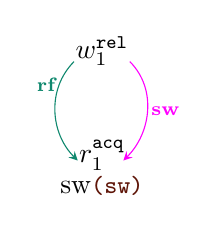
\begin{tikzpicture}[x=1em,y=1em,yscale=-1,xscale=-1]
\tikzstyle{every node}=[font=\normalfont]
\node (w1) {$ w^\rel_1 $};
\node (r1) [below=20pt of w1] {$ r^\acq_1 $};
\node (sw) [below=-5pt of r1] {\hlref{sw}};

\draw [->,>=stealth,color=Magenta] ($ (w1.south east)+(.3,-5pt) $) to[out=135,in=-135] node[midway,right=-2pt,font=\scriptsize] {\textcolor{black}{\lsw}} ($ (r1.south east)+(0.4,-7pt) $);
\draw [->,>=stealth,color=PineGreen] ($ (w1.south west)+(-.3,-5pt) $) to[out=45,in=-45] node[left=-2pt,pos=.25,font=\scriptsize] {\textcolor{black}{\lrf}}($ (r1.south west)+(-0.3,-7pt) $);

\end{tikzpicture}
} &
		\resizebox{0.14\textwidth}{!}{\tikzset{every picture/.style={line width=0.75pt}} %set default line width to 0.75pt        
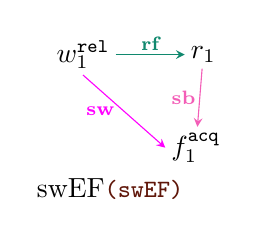
\begin{tikzpicture}[x=1em,y=1em,yscale=-1,xscale=-1]
\tikzstyle{every node}=[font=\normalfont]
\node (w1) [inner sep=2pt] {$ w^\rel_1 $};
\node (r1) [right=25pt of w1,inner sep=2pt] {$ r_1 $};
\node (f1) [below left=21pt and -15pt of r1,inner sep=2pt] {$ f^\acq_1 $};
\node (swef) [below left=0pt and -10pt of f1] {\hlref{swEF}};

`\draw [->,>=stealth,color=Magenta,thin] (w1.south) -- node[midway,left=0pt,font=\scriptsize,color=black] { $\lsw$ } (f1.west);
\draw [->,>=stealth,color=PineGreen,thin] (w1) -- node[midway,above=-2pt,font=\scriptsize,color=black] { $ \lrf $ }  (r1);
\draw [->,>=stealth,color=CarnationPink,thin] (r1) -- node[midway,left=-2pt,font=\scriptsize,color=black] { $\lsb$ } (f1);

\end{tikzpicture}
} &
		\resizebox{0.14\textwidth}{!}{\tikzset{every picture/.style={line width=0.75pt}} %set default line width to 0.75pt        
\begin{tikzpicture}[x=1em,y=1em,yscale=-1,xscale=-1]
\tikzstyle{every node}=[font=\normalfont]
\node [inner sep=2pt] (f1) {$ f^\rel_1 $};
\node (w1) [below left=21pt and -15pt of f1,inner sep=2pt] {$ w_1 $};
\node (r1) [right=25pt of w1,inner sep=2pt] {$ r^\acq_1 $};
\node (swfe) [below right=0pt and -15pt of wr1] {\hlref{sw-dobFE}};

`\draw [->,>=stealth,color=Magenta,thin] (f1.east) -- node[midway,right=0pt,font=\scriptsize,color=black] { $\lsw$ } (r1.north);
\draw [->,>=stealth,color=PineGreen,thin] (w1) -- node[midway,above=-2pt,font=\scriptsize,color=black] { $ \lrf $ } (r1);
\draw [->,>=stealth,color=CarnationPink,thin] (f1) -- node[midway,left=-2pt,font=\scriptsize,color=black] { $\lsb$ } (w1);

\end{tikzpicture}
} &
		\resizebox{0.17\textwidth}{!}{\tikzset{every picture/.style={line width=0.75pt}} %set default line width to 0.75pt        
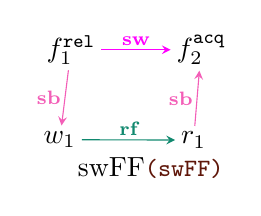
\begin{tikzpicture}[x=1em,y=1em,yscale=-1,xscale=-1]
\tikzstyle{every node}=[font=\normalfont]
\node (f1) [inner sep=2pt] {$ f^\rel_1 $};
\node (f2) [right=25pt of f1,inner sep=2pt] {$ f^\acq_2 $};
\node (w1) [below left=20pt and -15pt of f1,inner sep=2pt] {$ w_1 $};
\node (r1) [below left=20pt and -15pt of f2,inner sep=2pt] {$ r_1 $};
\node (swff) [below right=-2pt and -5pt of w1] {\hlref{swFF}};

`\draw [->,>=stealth,color=Magenta] (f1) -- node[midway,above=-2pt,font=\scriptsize,color=black] { $\lsw$ } (f2);
\draw [->,>=stealth,color=PineGreen] (w1) -- node[midway,above=-2pt,font=\scriptsize,color=black]{\lrf} (r1);
\draw [->,>=stealth,color=CarnationPink] (f1) -- node[midway,left=-2pt,font=\scriptsize,color=black] { $\lsb$ } (w1);
\draw [->,>=stealth,color=CarnationPink] (r1) -- node[midway,left=-2pt,font=\scriptsize,color=black] { $\lsb$ } (f2);

%\draw [->,>=stealth,color=orange] ($ (ew1.south east)+(.5,-5pt) $) to[out=135,in=-135] node[midway,right=-2pt,font=\scriptsize] {mo} ($ (ew2.south east)+(0.4,-5pt) $);
%\draw [->,>=stealth,color=red] ($ (ew1.south west)+(-.3,-5pt) $) to[out=45,in=-45] node[midway,left=-2pt,font=\scriptsize] {c::hb} ($ (ew2.south west)+(-0.3,-5pt) $);


\end{tikzpicture}
} &
		
		\resizebox{0.16\textwidth}{!}{\tikzset{every picture/.style={line width=0.75pt}} %set default line width to 0.75pt        
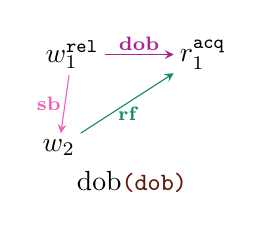
\begin{tikzpicture}[x=1em,y=1em,yscale=-1,xscale=-1]
\tikzstyle{every node}=[font=\normalfont]
\node (w1) [inner sep=2pt] {$ w^\rel_1 $};
\node (r1) [right=25pt of w1,inner sep=2pt] {$ r^\acq_1 $};
\node (w2) [below left=21pt and -15pt of w1,inner sep=2pt] {$ w_2 $};
\node (dob) [below right=0pt and -5pt of w2] {\hlref{dob}};

`\draw [->,>=stealth,color=Mulberry] (w1.east) -- node[midway,above=-2pt,font=\scriptsize,color=black] { $\ldob$ } (r1.west);
\draw [->,>=stealth,color=PineGreen] (w2) -- node[midway,below=-2pt,font=\scriptsize,color=black] { $ \lrf $ }  (r1);
\draw [->,>=stealth,color=CarnationPink] (w1) -- node[midway,left=-2pt,font=\scriptsize,color=black] { $\lsb$ } (w2);

\end{tikzpicture}
} &
		\resizebox{0.17\textwidth}{!}{\tikzset{every picture/.style={line width=0.75pt}} %set default line width to 0.75pt        
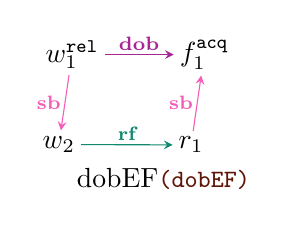
\begin{tikzpicture}[x=1em,y=1em,yscale=-1,xscale=-1]
\tikzstyle{every node}=[font=\normalfont]
\node (w1) [inner sep=2pt] {$ w^\rel_1 $};
\node (f1) [right=25pt of w1,inner sep=2pt] {$ f^\acq_1 $};
\node (w2) [below left=20pt and -15pt of w1,inner sep=2pt] {$ w_2 $};
\node (r1) [below left=20pt and -13pt of f1,inner sep=2pt] {$ r_1 $};
\node (dobEF) [below right=0pt and -5pt of w2] {\hlref{dobEF}};

`\draw [->,>=stealth,color=PineGreen,thin] (w2) -- node[midway,above=-2pt,font=\scriptsize,color=black] { $\lrf$ } (r1);
\draw [->,>=stealth,color=CarnationPink,thin] (w1) -- node[midway,left=-2pt,font=\scriptsize,color=black] { $ \lsb $ } (w2);
\draw [->,>=stealth,color=CarnationPink,thin] (r1) -- node[midway,left=-2pt,font=\scriptsize,color=black] { $\lsb$ } (f1);
\draw [->,>=stealth,color=Mulberry,thin] (w1) -- node[midway,above=-2pt,font=\scriptsize,color=black] { $\ldob$ } (f1);

\end{tikzpicture}
} \\
		\hline
		\multicolumn{4}{c}{(a) \lsw relation} &
		\multicolumn{2}{c}{(b) \ldob relation} \\
	\end{tabular}
	\label{fig:sw}
\end{figure}

\noindent
Formally, $\setSW$ relation is formed using fences as,

$\forall e_1, e_2 \in \events_\tau$ \st $\rf{\tau}{e_1}{e_2}$

if
$e_1 \in \ordwrites{\moge\rel}_\tau$, 
$\exists \mathbb{F}^\acq \in \ordfences{\moge\acq}_{\tau}$ where
$\seqb{\tau}{e_2}{\mathbb{F}^\acq}$ then
$\sw{\tau}{e_1}{\mathbb{F}^\acq}$;

if
$e_2 \in \ordreads{\moge\acq}_\tau$, 
$\exists \mathbb{F}^\rel \in \ordfences{\moge\rel}_{\tau}$ where
$\seqb{\tau}{\mathbb{F}^\rel}{e_1}$ then
$\sw{\tau}{\mathbb{F}^\rel}{e_2}$;

if
$\exists \mathbb{F}^\rel \in \ordfences{\moge\rel}_{\tau}$,
$\mathbb{F}^\acq \in \ordfences{\moge\acq}_{\tau}$ where
$\seqb{\tau}{\mathbb{F}^\rel}{e_1}$,
$\seqb{\tau}{e_2}{\mathbb{F}^\acq}$ 

then
$\sw{\tau}{\mathbb{F}^\rel}{\mathbb{F}^\acq}$.

\noindent
Similarly, $\setDOB$ relation is formed using fences as,

$\forall e_1, e_2 \in \events_\tau$, 
$e_1' \in \ordwrites{\moge\rel}_\tau$ \st $\rf{\tau}{e_1}{e_2}$
and $e_1 \in$ {\em release-sequence}($e_1'$)

if $\exists \mathbb{F}^\acq \in \ordfences{\moge\acq}_{\tau}$ 
where $\seqb{\tau}{e_2}{\mathbb{F}^\acq}$ then
$\dob{\tau}{e_1'}{\mathbb{F}^\acq}$.

\noindent
Further, as is the case with program events,
if $\sw{\tau}{e_1}{e_2}$ or $\dob{\tau}{e_1}{e_2}$ then
events $e_1',e_2'$ \st $\seqb{\tau}{e_1'}{e_1}$ and 
$\seqb{\tau}{e_2}{e_2'}$ are related as $\ithb{\tau}{e_1'}{e_2'}$.

\section{Invalidating buggy traces with \cc fences} \label{sec:invalidating ce}
As discussed in Section~\ref{sec:c11}, in a valid trace of the
input program $P$ (including a buggy trace), 
the program events must satisfy the \hlref{coherence conditions}.
%
Contrarily, if we synthesize \cc fences in the input program 
such that the irreflexivity of any of the coherence conditions 
or the total order on \sc events in the buggy trace gets violated 
then we can invalidate the trace and stop the program behavior.

Assume a set of synthesized \cc fences $\overline{\fences_{\tau'}}$
in a transformation $\tau'$ of a buggy trace $\tau$. 
%
The synthesized fences inflate the 
$\setSB$, $\setSW$ and $\setDOB$ relation sets by adding 
relations between program events ($\events_\tau$) and newly 
added fences ($\sfences_{\tau'}$) to form corresponding 
$\seqb{\tau'}{}{}$, $\sw{\tau'}{}{}$ and $\dob{\tau'}{}{}$ 
relations (as explained in Section~\ref{sec:c11}). 
%
Further, the $\ithb{\tau'}{}{}$ relation contains  
program event pairs as a consequence of the freshly formed 
$\sw{\tau'}{}{}$ and $\dob{\tau'}{}{}$ relations in addition
to the event pairs in $\setITHB$.
%
The $\mo{\tau'}{}{}$, $\rf{\tau'}{}{}$ and $\fr{\tau'}{}{}$ 
relations remain the same as the corresponding relations of 
$\tau$, as fences do not contribute to these relations.

We propose two strategies, namely \stfence and \wkfence, to 
detect invalidation of the program trace $\tau$. 
%
The \wkfence strategy detects violation of a coherence condition.
If such a case exists then we can stop the behavior by
synthesizing weaker fences (memory orders \rel, \acq, \acqrel). 
%
However, if a coherence condition is not violated then we move
to \stfence strategy to break the total order requirement on
\sc ordered events and stop the behavior by synthesizing 
strong (\sc ordered) fences.
%
The strategies are discussed below.\newline

\begin{figure}[t]
	\begin{tabular}{|c|c|c|}
		\hline
		\resizebox{0.33\textwidth}{!}{\tikzset{every picture/.style={line width=0.75pt}} %set default line width to 0.75pt        
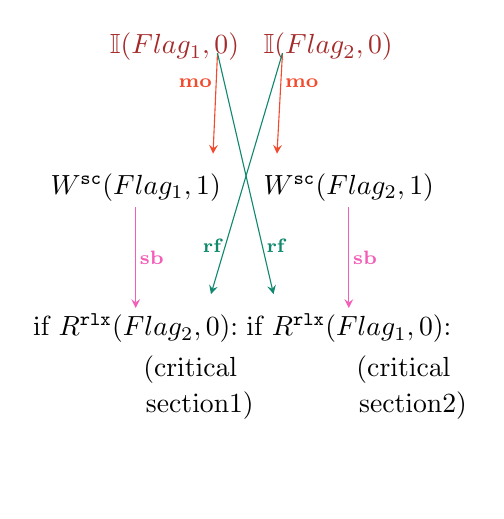
\begin{tikzpicture}[x=1em,y=1em,yscale=-1,xscale=-1]
	\tikzstyle{every node}=[font=\normalfont]
	
	\node (ifl1) [inner sep=2pt,color=Brown] {$\mathbb{I}(Flag_1,0)$};
	\node (ifl2) [right=30pt,inner sep=2pt,color=Brown] {$\mathbb{I}(Flag_2,0)$};
	
	\node (f11) [below left=10pt and -30pt of ifl1,inner sep=2pt,color=White] {$\mathbb{F}^\acqrel_{11}$};
	\node (fl1) [below=10pt of f11, inner sep=2pt] {$ W^\sc(Flag_1,1) $};
	\node (f12) [below=10pt of fl1, inner sep=2pt,color=White] {$\mathbb{F}^\acqrel_{12}$};
	\node (rfl2) [below=10pt of f12, inner sep=2pt] {if $R^\rlx(Flag_2,0)$:};
	\node (cs11) [below right=-1pt and -40pt of rfl2] {(critical};
	\node (cs12) [below right=-4pt and -40pt of cs11] {section1)};
	\node (f13) [below=35pt of rfl2, inner sep=2pt,color=White] {$\mathbb{F}^\acqrel_{13}$};
	
	\node (f21) [right=40pt of f11, inner sep=2pt,color=White] {$\mathbb{F}^\acqrel_{21}$};
	\node (fl2) [below=10pt of f21, inner sep=2pt] {$W^\sc(Flag_2,1)$};
	\node (f22) [below=10pt of fl2, inner sep=2pt,color=White] {$\mathbb{F}^\acqrel_{22}$};
	\node (rfl1) [below=10pt of f22, inner sep=2pt] {if $R^\rlx(Flag_1,0)$:};
	\node (cs21) [below right=-1pt and -40pt of rfl1] {(critical};
	\node (cs22) [below right=-4pt and -40pt of cs21] {section2)};
	\node (f23) [below=35pt of rfl1, inner sep=2pt,color=White] {$\mathbb{F}^\acqrel_{23}$};
	%
	\draw [->,>=stealth,color=RedOrange] ($ (ifl1.south east)+(1,-5pt) $) -- node[pos=0.3,left=-2pt,font=\scriptsize,color=black] { $\lmo$ } ($ (fl1.north east)+(0.5,-5pt) $);
	\draw [->,>=stealth,color=RedOrange] ($ (ifl2.south west)+(-0.9,-5pt) $) -- node[pos=0.3,right=-2pt,font=\scriptsize,color=black] { $\lmo$ } ($ (fl2.north west)+(-0.7,-5pt) $);
	
	\draw [->,>=stealth,color=CarnationPink] (fl1) -- node[midway,right=-2pt,font=\scriptsize,color=black] { $\lsb$ } (rfl2);
	\draw [->,>=stealth,color=CarnationPink] (fl2) -- node[midway,right=-2pt,font=\scriptsize,color=black] { $\lsb$ } (rfl1);
	
	\draw [->,>=stealth,color=PineGreen] ($ (ifl1.south east)+(1,-5pt) $) -- node[pos=0.8,right=-2pt,font=\scriptsize,color=black] { $\lrf$ } ($ (rfl1.north west)+(-1.2,-5pt) $);
	\draw [->,>=stealth,color=PineGreen] ($ (ifl2.south west)+(-0.9,-5pt) $) -- node[pos=0.8,left=-2pt,font=\scriptsize,color=black] { $\lrf$ } ($ (rfl2.north east)+(1.2,-5pt) $);
	
\end{tikzpicture}
} &
		\resizebox{0.33\textwidth}{!}{\tikzset{every picture/.style={line width=0.75pt}} %set default line width to 0.75pt        
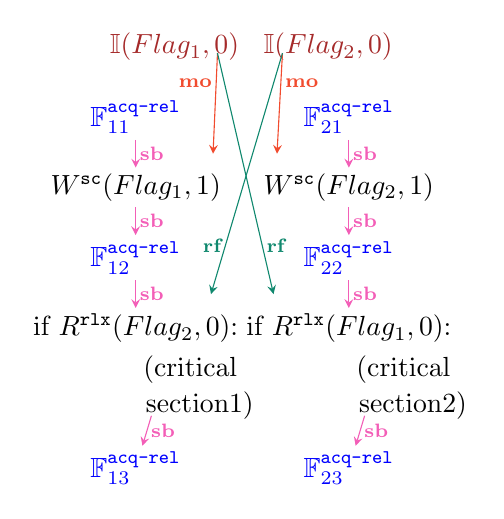
\begin{tikzpicture}[x=1em,y=1em,yscale=-1,xscale=-1]
\tikzstyle{every node}=[font=\normalfont]

\node (ifl1) [inner sep=2pt,color=Brown] {$\mathbb{I}(Flag_1,0)$};
\node (ifl2) [right=30pt,inner sep=2pt,color=Brown] {$\mathbb{I}(Flag_2,0)$};

\node (f11) [below left=10pt and -30pt of ifl1,inner sep=2pt,color=Blue] {$\mathbb{F}^\acqrel_{11}$};
\node (fl1) [below=10pt of f11, inner sep=2pt] {$ W^\sc(Flag_1,1) $};
\node (f12) [below=10pt of fl1, inner sep=2pt,color=Blue] {$\mathbb{F}^\acqrel_{12}$};
\node (rfl2) [below=10pt of f12, inner sep=2pt] {if $R^\rlx(Flag_2,0)$:};
\node (cs11) [below right=-1pt and -40pt of rfl2] {(critical};
\node (cs12) [below right=-4pt and -40pt of cs11] {section1)};
\node (f13) [below=35pt of rfl2, inner sep=2pt,color=Blue] {$\mathbb{F}^\acqrel_{13}$};

\node (f21) [right=40pt of f11, inner sep=2pt,color=Blue] {$\mathbb{F}^\acqrel_{21}$};
\node (fl2) [below=10pt of f21, inner sep=2pt] {$W^\sc(Flag_2,1)$};
\node (f22) [below=10pt of fl2, inner sep=2pt,color=Blue] {$\mathbb{F}^\acqrel_{22}$};
\node (rfl1) [below=10pt of f22, inner sep=2pt] {if $R^\rlx(Flag_1,0)$:};
\node (cs21) [below right=-1pt and -40pt of rfl1] {(critical};
\node (cs22) [below right=-4pt and -40pt of cs21] {section2)};
\node (f23) [below=35pt of rfl1, inner sep=2pt,color=Blue] {$\mathbb{F}^\acqrel_{23}$};
%
\draw [->,>=stealth,color=RedOrange] ($ (ifl1.south east)+(1,-5pt) $) -- node[pos=0.3,left=-2pt,font=\scriptsize,color=black] { $\lmo$ } ($ (fl1.north east)+(0.5,-5pt) $);
\draw [->,>=stealth,color=RedOrange] ($ (ifl2.south west)+(-0.9,-5pt) $) -- node[pos=0.3,right=-2pt,font=\scriptsize,color=black] { $\lmo$ } ($ (fl2.north west)+(-0.7,-5pt) $);

\draw [->,>=stealth,color=CarnationPink] (f11) -- node[midway,right=-2pt,font=\scriptsize,color=black] { $\lsb$ } (fl1);
\draw [->,>=stealth,color=CarnationPink] (fl1) -- node[midway,right=-2pt,font=\scriptsize,color=black] { $\lsb$ } (f12);
\draw [->,>=stealth,color=CarnationPink] (f12) -- node[midway,right=-2pt,font=\scriptsize,color=black] { $\lsb$ } (rfl2);
\draw [->,>=stealth,color=CarnationPink] ($ (cs12.south west)+(-0.55,-5pt) $) -- node[midway,right=-2pt,font=\scriptsize,color=black] { $\lsb$ } (f13);

\draw [->,>=stealth,color=CarnationPink] (f21) -- node[midway,right=-2pt,font=\scriptsize,color=black] { $\lsb$ } (fl2);
\draw [->,>=stealth,color=CarnationPink] (fl2) -- node[midway,right=-2pt,font=\scriptsize,color=black] { $\lsb$ } (f22);
\draw [->,>=stealth,color=CarnationPink] (f22) -- node[midway,right=-2pt,font=\scriptsize,color=black] { $\lsb$ } (rfl1);
\draw [->,>=stealth,color=CarnationPink] ($ (cs22.south west)+(-0.55,-5pt) $) -- node[midway,right=-2pt,font=\scriptsize,color=black] { $\lsb$ } (f23);

\draw [->,>=stealth,color=PineGreen] ($ (ifl1.south east)+(1,-5pt) $) -- node[pos=0.8,right=-2pt,font=\scriptsize,color=black] { $\lrf$ } ($ (rfl1.north west)+(-1.2,-5pt) $);
\draw [->,>=stealth,color=PineGreen] ($ (ifl2.south west)+(-0.9,-5pt) $) -- node[pos=0.8,left=-2pt,font=\scriptsize,color=black] { $\lrf$ } ($ (rfl2.north east)+(1.2,-5pt) $);

\end{tikzpicture}
} &
		\resizebox{0.33\textwidth}{!}{\tikzset{every picture/.style={line width=0.75pt}} %set default line width to 0.75pt        
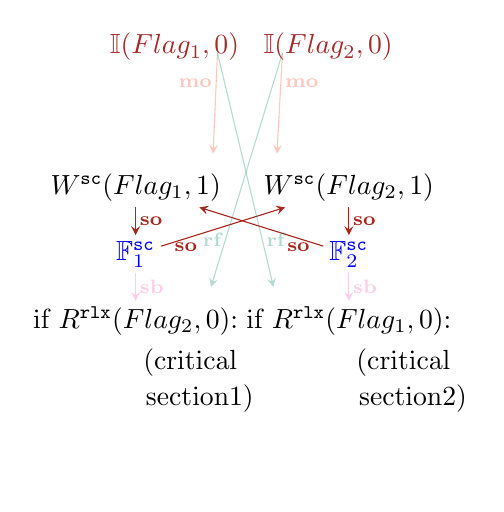
\begin{tikzpicture}[x=1em,y=1em,yscale=-1,xscale=-1]
	\tikzstyle{every node}=[font=\normalfont]
	
	\node (ifl1) [inner sep=2pt,color=Brown] {$\mathbb{I}(Flag_1,0)$};
	\node (ifl2) [right=30pt,inner sep=2pt,color=Brown] {$\mathbb{I}(Flag_2,0)$};
	
	\node (f11) [below left=10pt and -30pt of ifl1,inner sep=2pt,color=White] {$\mathbb{F}^\acqrel_{11}$};
	\node (fl1) [below=10pt of f11, inner sep=2pt] {$ W^\sc(Flag_1,1) $};
	\node (f12) [below=10pt of fl1, inner sep=2pt,color=Blue] {$\mathbb{F}^\sc_{1}$};
	\node (rfl2) [below=10pt of f12, inner sep=2pt] {if $R^\rlx(Flag_2,0)$:};
	\node (cs11) [below right=-1pt and -40pt of rfl2] {(critical};
	\node (cs12) [below right=-4pt and -40pt of cs11] {section1)};
	\node (f13) [below=35pt of rfl2, inner sep=2pt,color=White] {$\mathbb{F}^\acqrel_{13}$};
	
	\node (f21) [right=40pt of f11, inner sep=2pt,color=White] {$\mathbb{F}^\acqrel_{21}$};
	\node (fl2) [below=10pt of f21, inner sep=2pt] {$W^\sc(Flag_2,1)$};
	\node (f22) [below=10pt of fl2, inner sep=2pt,color=Blue] {$\mathbb{F}^\sc_{2}$};
	\node (rfl1) [below=10pt of f22, inner sep=2pt] {if $R^\rlx(Flag_1,0)$:};
	\node (cs21) [below right=-1pt and -40pt of rfl1] {(critical};
	\node (cs22) [below right=-4pt and -40pt of cs21] {section2)};
	\node (f23) [below=35pt of rfl1, inner sep=2pt,color=White] {$\mathbb{F}^\acqrel_{23}$};
	%
	\draw [->,>=stealth,color=RedOrange,opacity=0.3] ($ (ifl1.south east)+(1,-5pt) $) -- node[pos=0.3,left=-2pt,font=\scriptsize,color=black] { $\lmo$ } ($ (fl1.north east)+(0.5,-5pt) $);
	\draw [->,>=stealth,color=RedOrange,opacity=0.3] ($ (ifl2.south west)+(-0.9,-5pt) $) -- node[pos=0.3,right=-2pt,font=\scriptsize,color=black] { $\lmo$ } ($ (fl2.north west)+(-0.7,-5pt) $);
	
	\draw [->,>=stealth,color=Mahogany] (fl1) -- node[midway,right=-2pt,font=\scriptsize,color=black] { $\lso$ } (f12);
	\draw [->,>=stealth,color=CarnationPink,opacity=0.3] (f12) -- node[midway,right=-2pt,font=\scriptsize,color=black] { $\lsb$ } (rfl2);
	
	\draw [->,>=stealth,color=Mahogany] (fl2) -- node[midway,right=-2pt,font=\scriptsize,color=black] { $\lso$ } (f22);
	\draw [->,>=stealth,color=CarnationPink,opacity=0.3] (f22) -- node[midway,right=-2pt,font=\scriptsize,color=black] { $\lsb$ } (rfl1);
	
	\draw [->,>=stealth,color=Mahogany] (f12) -- node[pos=0.2,below=-2pt,font=\scriptsize,color=black] { $\lso$ } (fl2);
	\draw [->,>=stealth,color=Mahogany] (f22) -- node[pos=0.2,below=-2pt,font=\scriptsize,color=black] { $\lso$ } (fl1);
	
	\draw [->,>=stealth,color=PineGreen,opacity=0.3] ($ (ifl1.south east)+(1,-5pt) $) -- node[pos=0.8,right=-2pt,font=\scriptsize,color=black] { $\lrf$ } ($ (rfl1.north west)+(-1.2,-5pt) $);
	\draw [->,>=stealth,color=PineGreen,opacity=0.3] ($ (ifl2.south west)+(-0.9,-5pt) $) -- node[pos=0.8,left=-2pt,font=\scriptsize,color=black] { $\lrf$ } ($ (rfl2.north east)+(1.2,-5pt) $);
	
\end{tikzpicture}
} \\
		\hline
		\multicolumn{1}{c}{\hl{mutex}} &
		\multicolumn{1}{c}{\hl{mutex-fences}} &
		\multicolumn{1}{c}{\hl{mutex-invalidated}} 
	\end{tabular}
\end{figure}

\noindent
{\bf Invalidate by violating coherence condition (\wkfence)}\newline
The \wkfence strategy simply attempts to detect a cycle in 
one of the \hlref{coherence conditions} listed in 
Section~\ref{sec:c11}.
%
Consider the example \hlref{WRIR}. Since, the trace does not 
violate any coherence condition it is a valid trace under \cc. 
Assume that the trace shown in the figure is a counter example.
%
Synthesizing release fence $\mathbb{F^\rel}$ and acquire fence 
$\mathbb{F^\acq}$ as shown in \hlref{WRIR-invalidated} forms
a cycle in $\setMO;\setRF;\setHB;\setRF^{-1}$ thus violating the
coherence of the trace.
%
\begin{figure}[h]
	\begin{tabular}{|c|c|}
		\hline
		\resizebox{0.5\textwidth}{!}{\tikzset{every picture/.style={line width=0.75pt}} %set default line width to 0.75pt        
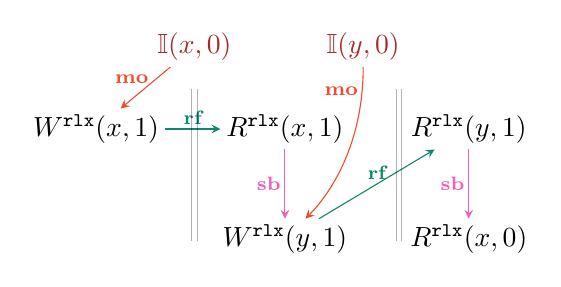
\begin{tikzpicture}[x=1em,y=1em,yscale=-1,xscale=-1]
\tikzstyle{every node}=[font=\normalfont]
\node (ix) [inner sep=2pt,color=Brown] {$\mathbb{I}(x,0)$};
\node (iy) [right=30pt of ix, inner sep=2pt,color=Brown] {$\mathbb{I}(y,0)$};
\node (wx) [below left=15pt and -5pt of ix, inner sep=2pt] {$ W^\rlx(x,1)$};
\node (rx1) [right=20pt of wx, inner sep=2pt] {$R^\rlx(x,1)$};
\node (wy) [below=25pt of rx1, inner sep=2pt] {$W^\rlx(y,1)$};
\node (ry) [right=20pt of rx1, inner sep=2pt] {$R^\rlx(y,1)$};
\node (rx0) [below=25pt of ry, inner sep=2pt] {$R^\rlx(x,0)$};
%
\draw [->,>=stealth,color=RedOrange] (ix) -- node[pos=0.3,left=-1pt,font=\scriptsize,color=black] { $\lmo$ } (wx);
\draw [->,>=stealth,color=RedOrange] (iy.south) to[in=-135,out=90] node[pos=0.1,left=-2pt,font=\scriptsize,color=black] { $\lmo$ } (wy);
\draw [->,>=stealth,color=PineGreen] (wx) -- node[midway,above=-2pt,font=\scriptsize,color=black] { $\lrf$ } (rx1);
\draw [->,>=stealth,color=CarnationPink] (rx1) -- node[midway,left=-2pt,font=\scriptsize,color=black] { $\lsb$ } (wy);
\draw [->,>=stealth,color=PineGreen] (wy) -- node[midway,above=-2pt,font=\scriptsize,color=black] { $\lrf$ } (ry);
\draw [->,>=stealth,color=CarnationPink] (ry) -- node[midway,left=-2pt,font=\scriptsize,color=black] { $\lsb$ } (rx0);

\draw [opacity=0.3] (-0.1,1.5) -- (-0.1,7);
\draw [opacity=0.3] (0.1,1.5) -- (0.1,7);

\draw [opacity=0.3] (-7.3,1.5) -- (-7.3,7);
\draw [opacity=0.3] (-7.5,1.5) -- (-7.5,7);

\end{tikzpicture}
} &
		\resizebox{0.5\textwidth}{!}{\tikzset{every picture/.style={line width=0.75pt}} %set default line width to 0.75pt        
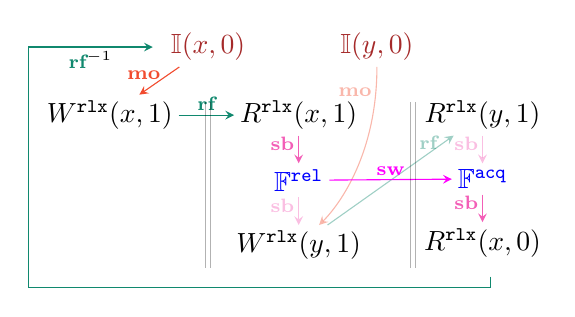
\begin{tikzpicture}[x=1em,y=1em,yscale=-1,xscale=-1]
\tikzstyle{every node}=[font=\normalfont]

\node (ix) [inner sep=2pt,color=Brown] {$\mathbb{I}(x,0)$};
\node (iy) [right=30pt of ix, inner sep=2pt,color=Brown] {$\mathbb{I}(y,0)$};
\node (wx) [below left=10pt and -5pt of ix, inner sep=2pt] {$ W^\rlx(x,1)$};
\node (rx1) [right=20pt of wx, inner sep=2pt] {$R^\rlx(x,1)$};
\node (frel) [below=10pt of rx1, inner sep=2pt,color=Blue] {$\mathbb{F}^\rel$};
\node (wy) [below=10pt of frel, inner sep=2pt] {$W^\rlx(y,1)$};
\node (ry) [right=20pt of rx1, inner sep=2pt] {$R^\rlx(y,1)$};
\node (facq) [below=10pt of ry, inner sep=2pt,color=Blue] {$\mathbb{F}^\acq$};
\node (rx0) [below=10pt of facq, inner sep=2pt] {$R^\rlx(x,0)$};
%
\draw [->,>=stealth,color=RedOrange] (ix) -- node[pos=0.3,left=-1pt,font=\scriptsize,color=black] { $\lmo$ } (wx);
\draw [->,>=stealth,color=RedOrange,opacity=0.4] (iy.south) to[in=-135,out=90] node[pos=0.1,left=-2pt,font=\scriptsize,color=black] { $\lmo$ } (wy);
\draw [->,>=stealth,color=PineGreen] (wx) -- node[midway,above=-2pt,font=\scriptsize,color=black] { $\lrf$ } (rx1);
\draw [->,>=stealth,color=CarnationPink] (rx1) -- node[pos=0.3,left=-2pt,font=\scriptsize,color=black] { $\lsb$ } (frel);
\draw [->,>=stealth,color=CarnationPink,opacity=0.4] (frel) -- node[pos=0.3,left=-2pt,font=\scriptsize,color=black] { $\lsb$ } (wy);
\draw [->,>=stealth,color=PineGreen,opacity=0.4] (wy) -- node[pos=0.8,above=-2pt,font=\scriptsize,color=black] { $\lrf$ } (ry);
\draw [->,>=stealth,color=CarnationPink,opacity=0.4] (ry) -- node[pos=0.3,left=-2pt,font=\scriptsize,color=black] { $\lsb$ } (facq);
\draw [->,>=stealth,color=CarnationPink] (facq) -- node[pos=0.3,left=-2pt,font=\scriptsize,color=black] { $\lsb$ } (rx0);
\draw [->,>=stealth,color=Magenta] (frel) -- node[midway,above=-2pt,font=\scriptsize,color=black] { \lsw } (facq);
\draw [color=PineGreen] (-10.2,8.3) -- (-10.2,8.7);
\draw [color=PineGreen] (6.5,8.7) -- (-10.2,8.7);
\draw [color=PineGreen] (6.5,0) -- (6.5,8.7);
\draw [->,>=stealth,color=PineGreen] (6.5,0) -- node[midway,below=-2pt,font=\scriptsize,color=black] { $\lrf^{-1}$ } (2,0);

\draw [opacity=0.3] (-0.1,2) -- (-0.1,8);
\draw [opacity=0.3] (0.1,2) -- (0.1,8);

\draw [opacity=0.3] (-7.3,2) -- (-7.3,8);
\draw [opacity=0.3] (-7.5,2) -- (-7.5,8);

\end{tikzpicture}
} \\
		\hline
		\multicolumn{1}{c}{\hl{WRIR}} &
		\multicolumn{1}{c}{\hl{WRIR-invalidated}}
	\end{tabular}
\end{figure}

However, inserting fences in a buggy trace may not be sufficient for 
violating a coherence condition. Consider example \hlref{mutex} and
its transformation \hlref{mutex-fences} with synthesized fences. 
%
As can be seen from \hlref{mutex-fences}, even after inserting fences 
at every location in the buggy trace, the trace still satisfies all 
coherence conditions and is thus valid.
\newline

\noindent
{\bf Invalidating by violating \sc total-order (\stfence)}\newline
If the \wkfence strategy fails to invalidate the buggy trace then
we attempt to violate the total-order on \sc events.
%
Since the coherence condition did on violate on the events of $\tau'$ 
it implies that conditions do not violate on the \sc ordered events
of $\tau'$ either. 
%
As a result in the \stfence strategy we attempt to violate the 
irreflexivity condition on 
$(\onsc{\hb{\tau'}{}{}}$ $\union$ $\onsc{\mo{\tau'}{}{}}$ $\union$ 
$\onsc{\rf{\tau'}{}{}}$ $\union$ $\onsc{\fr{\tau'}{}{}})^+$. 

We introduce a possibly reflexive relation on \sc-ordered
events of $\tau'$, called {\em \sc-order} $(\so{\tau'}{}{})$ to 
capture the ordering between the \sc events. 
%
\begin{definition}{\bf \sc-order ($\so{\tau'}{}{}$)}\newline
	$\forall e_1, e_2 \in \events_\tau$ \st 
	$(e_1,e_2) \in$ $\setHB$ $\union$ $\setMO$ $\union$ $\setRF$ 
	$\union$ $\setFR$
	
	if
	$e_1, e_2 \in \ordevents{\sc}_\tau$ then 
	$\so{\tau'}{e_1}{e_2}$;
	
	if
	$e_1 \in \ordevents{\sc}_\tau$, 
	$\exists \mathbb{F}^\sc \in \ordsfences{\sc}_{\tau'}$ where
	$\seqb{\tau'}{e_2}{\mathbb{F}^\sc}$ then
	$\so{\tau'}{e_1}{\mathbb{F}^\sc}$;
	
	if
	$e_2 \in \ordevents{\sc}_\tau$, 
	$\exists \mathbb{F}^\sc \in \ordsfences{\sc}_{\tau'}$ where
	$\seqb{\tau'}{\mathbb{F}^\sc}{e_1}$ then
	$\so{\tau'}{\mathbb{F}^\sc}{e_2}$;
	
	if
	$\exists \mathbb{F}^\sc_1$, $\mathbb{F}^\sc_2$ 
	$\in \ordsfences{\sc}_{\tau'}$ where
	$\seqb{\tau'}{\mathbb{F}^\sc_1}{e_1}$ and 
	$\seqb{\tau'}{e_2}{\mathbb{F}^\sc_2}$ then
	$\so{\tau'}{\mathbb{F}^\sc_1}{\mathbb{F}^\sc_1}$.
\end{definition}
%
Note that, $\setSO \subseteq \setTO$ for any trace $\tau$. It
does not contain pairs of \sc events that do not have a definite
order. 
%
Consider the example \hlref{WRWR}, $\to{}{W^\sc(x,1)}{W^\sc(y,1)}$
and $\to{}{W^\sc(y,1)}{W^\sc(x,1)}$ are both valid total-orders
on the \sc events of the trace.
%
The set $\setSO$ does not contain either of the two cases and 
would be empty for this example.
%
Such a candidate pair of events cannot contribute to the 
reflexivity of $\setSO$ and can be safely ignored for the
purpose of this work. 
\setlength{\textfloatsep}{0pt}
%\begin{wrapfigure}{l}{0.3\textwidth}
%	\vspace{-2em}
%	\begin{tabular}{|c|}
%		\hline
%		\resizebox{0.3\textwidth}{!}{\tikzset{every picture/.style={line width=0.75pt}} %set default line width to 0.75pt        
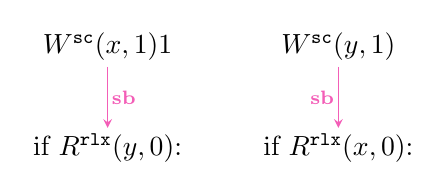
\begin{tikzpicture}[x=1em,y=1em,yscale=-1,xscale=-1]
\tikzstyle{every node}=[font=\normalfont]
\node (fl1) [inner sep=2pt] {$ W^\sc(x,1) 1 $};
\node (fl2) [right=35pt of fl1, inner sep=2pt] {$W^\sc(y,1)$};
\node (rfl2) [below=22pt of fl1, inner sep=2pt] {if $R^\rlx(y,0)$:};
\node (rfl1) [below=22pt of fl2, inner sep=2pt] {if $R^\rlx(x,0)$:};
%
\draw [->,>=stealth,color=CarnationPink] (fl1) -- node[midway,right=-2pt,font=\scriptsize,color=black] { $\lsb$ } (rfl2);
\draw [->,>=stealth,color=CarnationPink] (fl2) -- node[midway,left=-2pt,font=\scriptsize,color=black] { $\lsb$ } (rfl1);

\end{tikzpicture}
} \\
%		\hline
%		\multicolumn{1}{c}{\hl{WRWR}}
%	\end{tabular}
%\end{wrapfigure}
\begin{figure}[h]
	\begin{tabular}{|c|}
		\hline
		\resizebox{0.3\textwidth}{!}{\tikzset{every picture/.style={line width=0.75pt}} %set default line width to 0.75pt        
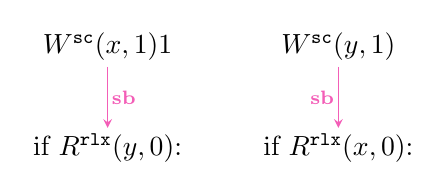
\begin{tikzpicture}[x=1em,y=1em,yscale=-1,xscale=-1]
\tikzstyle{every node}=[font=\normalfont]
\node (fl1) [inner sep=2pt] {$ W^\sc(x,1) 1 $};
\node (fl2) [right=35pt of fl1, inner sep=2pt] {$W^\sc(y,1)$};
\node (rfl2) [below=22pt of fl1, inner sep=2pt] {if $R^\rlx(y,0)$:};
\node (rfl1) [below=22pt of fl2, inner sep=2pt] {if $R^\rlx(x,0)$:};
%
\draw [->,>=stealth,color=CarnationPink] (fl1) -- node[midway,right=-2pt,font=\scriptsize,color=black] { $\lsb$ } (rfl2);
\draw [->,>=stealth,color=CarnationPink] (fl2) -- node[midway,left=-2pt,font=\scriptsize,color=black] { $\lsb$ } (rfl1);

\end{tikzpicture}
} \\
		\hline
		\multicolumn{1}{c}{\hl{WRWR}}
	\end{tabular}
\end{figure}

Consider again the example \hlref{mutex} without synthesized fences.
Upon synthesizing \sc fences $\mathbb{F}^\sc_1$ and 
$\mathbb{F}^\sc_2$ as shown in \hlref{mutex-invalidated} the
transformed trace forms the following $\so{}{}{}$ relations,

$\seqb{}{W^\sc(Flag_1,1)}{\mathbb{F}^\sc_1}$ $\implies$ $\so{}{W^\sc(Flag_1,1)}{\mathbb{F}^\sc_1}$

$\seqb{}{W^\sc(Flag_2,1)}{\mathbb{F}^\sc_2}$ $\implies$ $\so{}{W^\sc(Flag_2,1)}{\mathbb{F}^\sc_2}$

$\fr{}{R^\rlx(Flag_1,0)}{W^\sc(Flag_1,1)}$ $\implies$ $\so{}{\mathbb{F}^\sc_2}{W^\sc(Flag_1,1)}$

$\fr{}{R^\rlx(Flag_2,0)}{W^\sc(Flag_2,1)}$ $\implies$ $\so{}{\mathbb{F}^\sc_1}{W^\sc(Flag_2,1)}$,

thus violating the total-order requirement on \sc events and
invalidating the trace with strong fences.

\ourtechnique, thus, attempts to stop a buggy trace from
manifesting as an execution by synthesizing fences to 
invalidate the trace, by using either the \wkfence or 
\stfence strategy.
%
However, 
as discussed in Section~\ref{sec:c11} \cc fences are weak
fences.
%
It is noteworthy that introducing \cc fences in a program 
with weakly ordered events may not impose strong enough
reordering restrictions as strongly ordered events would.
%
As a consequence, it may be possible to stop a buggy 
trace by modifying the memory orders of program events
to stricter orders but fail to stop the same by 
inserting even the strictest \cc fences.

\begin{figure}[h]
	\begin{tabular}{|c|c|}
		\hline
		\resizebox{0.49\textwidth}{!}{\tikzset{every picture/.style={line width=0.75pt}} %set default line width to 0.75pt        
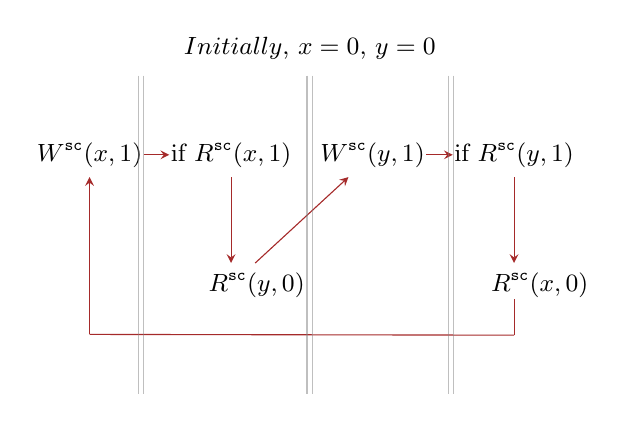
\begin{tikzpicture}[x=1em,y=1em,yscale=1,xscale=1]
\tikzstyle{every node}=[font=\small]

% other nodes
\node (init) {$Initially$, $x=0$, $y=0$};
\node (f11) [below left=0pt and 20pt of init,color=White] { $F^\sc_{11}$ };
\node (wx1) [below=8pt of f11] {$ W^\sc(x,1) $};
\node (f12) [below=8pt of wx1,color=White] { $F^\sc_{12}$ };

\node (f21) [right=30pt of f11,color=White] { $F^\sc_{21}$ };
\node (rx1) [below=8pt of f21] {if $ R^\sc(x,1) $};
\node (f22) [below=8pt of rx1,color=White] { $F^\sc_{22}$ };
\node (ry0) [below=8pt of f22] {\tab$ R^\sc(y,0) $};
\node (f23) [below=8pt of ry0,color=White] { $F^\sc_{23}$ };

\node (f31) [right=30pt of f21,color=White] { $F^\sc_{31}$ };
\node (wy1) [below=8pt of f31] {$ W^\sc(y,1) $};
\node (f32) [below=8pt of wy1,color=White] { $F^\sc_{32}$ };

\node (f41) [right=30pt of f31,color=White] { $F^\sc_{41}$ };
\node (ry1) [below=8pt of f41] {if $ R^\sc(y,1) $};
\node (f42) [below=8pt of ry1,color=White] { $F^\sc_{42}$ };
\node (rx0) [below=8pt of f42] {\tab$ R^\sc(x,0) $};
\node (f43) [below=8pt of rx0,color=White] { $F^\sc_{43}$ };

\draw [->,>=stealth,color=Brown] (rx1) -- (ry0);
\draw [->,>=stealth,color=Brown] (ry1) -- (rx0);

\draw [->,>=stealth,color=Brown] ($ (wx1.east)+(-3pt,0) $) -- ($ (rx1.west)+(3pt,0) $);
\draw [->,>=stealth,color=Brown] (ry0) -- (wy1);
\draw [->,>=stealth,color=Brown] ($ (wy1.east)+(-3pt,0) $) -- ($ (ry1.west)+(3pt,0) $);
\draw [color=Brown] (rx0.south)+(0,3pt) -- ($ (rx0.south)+(0,-10pt) $);
\draw [color=Brown] ($ (rx0.south)+(0,-10pt) $) -- ($ (wx1.south)+(0,-56.85pt) $);
\draw [->,>=stealth,color=Brown] ($ (wx1.south)+(0,-56.85pt) $) -- (wx1);

\draw [gray,opacity=0.5] (-6.2,-1.0) -- (-6.2,-12.5);
\draw [gray,opacity=0.5] (-6.0,-1.0) -- (-6.0,-12.5);

\draw [gray,opacity=0.5] (-0.1,-1.0) -- (-0.1,-12.5);
\draw [gray,opacity=0.5] (0.1,-1.0) -- (0.1,-12.5);

\draw [gray,opacity=0.5] (5.0,-1.0) -- (5.0,-12.5);
\draw [gray,opacity=0.5] (5.2,-1.0) -- (5.2,-12.5);

\end{tikzpicture}
} &
		\resizebox{0.49\textwidth}{!}{\tikzset{every picture/.style={line width=0.75pt}} %set default line width to 0.75pt        
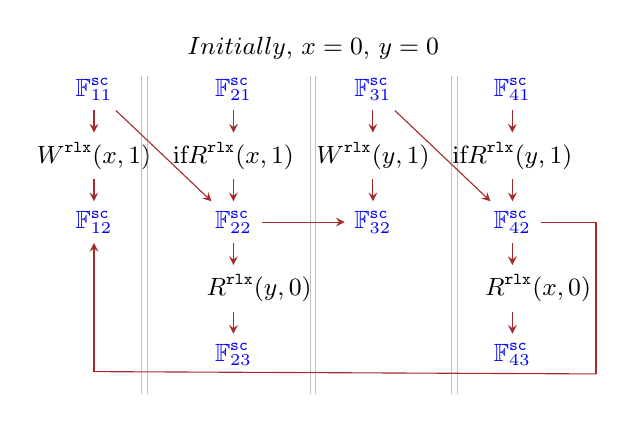
\begin{tikzpicture}[x=1em,y=1em,yscale=1,xscale=1]
\tikzstyle{every node}=[font=\small]

% other nodes
\node (init) {$Initially$, $x=0$, $y=0$};
\node (f11) [below left=0pt and 20pt of init,color=Blue] { $\mathbb{F}^\sc_{11}$ };
\node (wx1) [below=8pt of f11] {$ W^\rlx(x,1) $};
\node (f12) [below=8pt of wx1,color=Blue] { $\mathbb{F}^\sc_{12}$ };

\node (f21) [right=30pt of f11,color=Blue] { $\mathbb{F}^\sc_{21}$ };
\node (rx1) [below=8pt of f21] {if$ R^\rlx(x,1) $};
\node (f22) [below=8pt of rx1,color=Blue] { $\mathbb{F}^\sc_{22}$ };
\node (ry0) [below=8pt of f22] {\tab$ R^\rlx(y,0) $};
\node (f23) [below=8pt of ry0,color=Blue] { $\mathbb{F}^\sc_{23}$ };

\node (f31) [right=30pt of f21,color=Blue] { $\mathbb{F}^\sc_{31}$ };
\node (wy1) [below=8pt of f31] {$ W^\rlx(y,1) $};
\node (f32) [below=8pt of wy1,color=Blue] { $\mathbb{F}^\sc_{32}$ };

\node (f41) [right=30pt of f31,color=Blue] { $\mathbb{F}^\sc_{41}$ };
\node (ry1) [below=8pt of f41] {if$ R^\rlx(y,1) $};
\node (f42) [below=8pt of ry1,color=Blue] { $\mathbb{F}^\sc_{42}$ };
\node (rx0) [below=8pt of f42] {\tab$ R^\rlx(x,0) $};
\node (f43) [below=8pt of rx0,color=Blue] { $\mathbb{F}^\sc_{43}$ };

\draw [->,>=stealth,color=Brown] (f11) -- (wx1);
\draw [->,>=stealth,color=Brown] (wx1) -- (f12);

\draw [->,>=stealth,color=Brown] (f21) -- (rx1);
\draw [->,>=stealth,color=Brown] (rx1) -- (f22);
\draw [->,>=stealth,color=Brown] (f22) -- (ry0);
\draw [->,>=stealth,color=Brown] (ry0) -- (f23);

\draw [->,>=stealth,color=Brown] (f31) -- (wy1);
\draw [->,>=stealth,color=Brown] (wy1) -- (f32);

\draw [->,>=stealth,color=Brown] (f41) -- (ry1);
\draw [->,>=stealth,color=Brown] (ry1) -- (f42);
\draw [->,>=stealth,color=Brown] (f42) -- (rx0);
\draw [->,>=stealth,color=Brown] (rx0) -- (f43);

\draw [->,>=stealth,color=Brown] (f11) -- (f22);
\draw [->,>=stealth,color=Brown] (f22) -- (f32);
\draw [->,>=stealth,color=Brown] (f31) -- (f42);
\draw [color=Brown] (f42.east)+(0,0) -- ($ (f42.east)+(20pt,0) $);
\draw [color=Brown] (f42.east)+(20pt,0) -- ($ (f43.east)+(20pt,-7pt) $);
\draw [color=Brown] ($ (f43.east)+(20pt,-7pt) $) -- ($ (f12.south)+(0,-46.5pt) $);
\draw [->,>=stealth,color=Brown] ($ (f12.south)+(0,-46.5pt) $) -- (f12);

\draw [gray,opacity=0.5] (-6.2,-1.0) -- (-6.2,-12.5);
\draw [gray,opacity=0.5] (-6.0,-1.0) -- (-6.0,-12.5);

\draw [gray,opacity=0.5] (-0.1,-1.0) -- (-0.1,-12.5);
\draw [gray,opacity=0.5] (0.1,-1.0) -- (0.1,-12.5);

\draw [gray,opacity=0.5] (5.0,-1.0) -- (5.0,-12.5);
\draw [gray,opacity=0.5] (5.2,-1.0) -- (5.2,-12.5);

\end{tikzpicture}
} \\
		\hline
		\multicolumn{1}{c}{\hl{iriw-invalid}} & 
		\multicolumn{1}{c}{\hl{iriw-valid}}
	\end{tabular}
\end{figure}
The examples \hlref{iriw-invalid} and \hlref{iriw-valid} 
highlight the difference. As we can see in \hlref{iriw-valid},
the trace cannot be invalidated by \cc fences but the same 
can be achieved by changing the memory order of read and 
write events as shown in \hlref{iriw-invalid}.
%
%Consider the example \hlref{iriw-invalid}, the trace shown in
%figure is not a valid \cc trace as we cannot form a total 
%order on the \sc program events that agrees with the other event
%relations. The Figure~\hlref{iriw-valid} shows a version 
%of the example where the read and write events are \rlx ordered,
%under such a setting there is no possible placement of 
%program fences that can stop the trace.
%
\ourtechnique attempts to invalidate traces by synthesizing 
\cc fences, thus, buggy
traces such as \hlref{iriw-valid}, without the fences shown 
in the figure, cannot be stopped by \ourtechnique.

\section{Methodology} \label{sec:methodology}
Given a buggy input program $P$, \ourtechnique attempts to 
stop the buggy traces or counter examples (traces with 
assert statement violations) of $P$ by inserting \cc fences.
%
To do so the technique must accomplish three objectives
(O1) determine whether the buggy trace can be stopped by 
synthesizing \cc fences,
(O2) determine the placement of optimal number of synthesized 
fences (\ie the least number of program locations where fences 
must be synthesized that is sufficient to stop the trace), 
and
(O3) determine the optimal memory order of the synthesized 
fences (\ie the weakest memory order of synthesized fences 
that is sufficient to stop the trace).
%
We present the \ourtechnique-algorithm (Algorithm
\ref{alg:main algo}) that realizes the three objectives.
The algorithm takes a \cc program as input
and determines the optimal fence placement that can stop
the buggy traces of the input program or determines that
the program cannot be made bug-free with \cc fences.

\begin{algorithm}[h]
	\caption{Fence Synthesis}
	\label{alg:main algo}
	\DontPrintSemicolon
	\SetAlgoLined
	
	\SetKwFunction{Fmain}{\ourtechnique}
	\SetKwFunction{Fceg}{generateCounterExamples}
	\SetKwFunction{FcandidateF}{candidateFences}
	\SetKwFunction{Frel}{computeRelations}
	\SetKwFunction{Fwk}{weakFensying}
	\SetKwFunction{Fst}{strongFensying}
	\SetKwFunction{Fmin}{minModel}
	
	\SetKwData{satquery}{$\Phi$}
	\SetKwData{ce}{CE}
	\SetKwData{wk}{weakCycles}
	\SetKwData{st}{strongCycles}
	
	\SetKwProg{Fn}{Function}{:}{}
	
	\Fn{\Fmain{input program $P$}}{		
		\satquery $:=$ $\top$\;
		\ce $:=$ \Fceg{$P$}\;
		\ForAll(\tcc*[f]{$\tau = \langle \events_\tau, \setHB, \setMO, \setRF \rangle$}) {$\tau \in$ \ce}{
			$\events_{\imm{\tau}}$ $:=$ $\events_\tau$ $\union$ \FcandidateF{$\tau$}\;
			$(\hb{\imm{\tau}}{}{}, \mo{\imm{\tau}}{}{}, \rf{\imm{\tau}}{}{}, \rfinv{\imm{\tau}}{}{}, \fr{\imm{\tau}}{}{})$ 
				$:=$ \Frel{$\tau,\events_{\imm{\tau}}$}\;
			\wk $:=$ \Fwk{$\imm{\tau}$}\;
			\st $:=$ \Fst{$\imm{\tau}$}\;
			\If{\wk $= \emptyset$ $\^$ \st $= \emptyset$} {
				\KwRet $\emptyset$
				\tcc*{cannot stop $\tau$}
			}			
		}
	
		\satquery $:=$ \satquery $\^$ $\formula{$\wk $\v$ \st$}$\;
		\KwRet \Fmin{\satquery}
	}
		
		
%		\State 
%		\State $ \seqb{\imm{\tau}}{}{} := $ computeSB($\setSB, \events_{\imm{\tau}}$) \State $ \so{\tau^{\mathtt{im}}}{}{} := $ computeSO($\events_{\imm{\tau}}, \setHB, \setMO, \setRF, \seqb{\imm{\tau}}{}{}$)
%		\State cycles := computeCycles($ \so{\imm{\tau}}{}{} $)
%		\If {cycles == $ \emptyset $}
%		\State \texttt{Abort} (``This trace can't be stopped using \cc fences.'')
%		\State \Return
%		\EndIf
%		\State $\phi := \phi\ \^ \formula{\so{\imm{\tau}}{}{}} $ 
%		%			\State $ \phi := \phi_\tau $
%		\EndFor
%		\State F:= MinModel($ \phi $)
%		\State \Return F



%		% no enabled events left ie maximal sequence explored
%		\lIf{\FunexploredEv{$\tau$} = $\emptyset$}{\KwRet 
%			\tcc*[f]{maximal sequence explored}}
%		
%		% if there is no sequence and no constraint sequence
%		\If(\tcc*[f]{find next event to explore}){$S = \emptysequence$}{
%			\If(\tcc*[f]{multiple leads possible}){
%				$\exists (e_r, e_w) \in$ \FunexploredRW{$\tau, F$}}{
%				\lForAll{$e_w' \in \ui{\tau}{F}{e_r}$}{
%					\Fupdate($\tau, e_w', F$)
%				}
%				\nexte := $e_r$
%			}
%			\lElse{
%				\nexte := any event $\in$ \FunexploredEv{$\tau$};
%			}
%			
%			% updateLeads wrt to selected event
%			\Fupdate($\tau$, \nexte, $F$)
%		}
%		
%		% there is a sequence to be explored
%		\lElse{
%			\nexte := $\hd{S}$
%		}
%		
%		%		\lIf(\tcc*[f]{if no branch explore \nexte})
%		\lIf
%		{$S = \emptysequence \^$ \FunexploredLd{$\tau$} = $\emptyset$}{
%			$\ld{\s{\tau}} \cunioneq (\emptysequence,\ \seq{${\nexte}$},\ F)$
%		}
%		
%		\lElseIf(\tcc*[f]{explore next event in $S$}){$S \neq \emptysequence$}{
%			$\ld{\s{\tau}} \cunioneq (\emptysequence,\ S,\ F)$
%		}
%		
%		\While(\tcc*[f]{explore all leads})
%		{$\exists l \in$ \FunexploredLd{$\tau$}}{
%			\nextseq := $l^s \cmerge l^c$\;
%			\Dprime := $\{\tau' \| \hd{${\nextseq}$}.\tau' \in Dn(\s{\tau})\}$\;
%			\Fexplore{$\tau.\hd{${\nextseq}$},\ \tl{${\nextseq}$}$, \Dprime, $l^F$}\;
%			$\dn{\s{\tau}} \unioneq$ \nextseq
%		}
%	}
\end{algorithm}
\divComment{Can we give termination guarantee?}

\noindent
{\bf Algorithm~\ref{alg:main algo} overview:} 
The algorithm assumes the knowledge of the set of counter
examples in the form of traces (\ie a set of events and 
the sets of relations on the events, as defined in Section
\ref{sec:preliminaries}).
%
Broadly the algorithm places candidate fences before and
after every program event then works towards eliminating 
fences that do not contribute to the optimal solution.
%
The elimination is a two-phase process where in the first
phase the algorithm discards candidate fences that do not 
contribute to the violation of either a coherence condition 
or the \sc total order. 
Further, in the second phase the algorithm reduces the 
remaining candidate fences to the optimal number with
the optimal memory order.

The algorithm takes a \cc program as input and relies on a 
counter example generator to return the set of counter 
examples or buggy traces of the input program (line 3).
It then transforms the buggy traces $\tau$ to an intermediate 
trace $\imm{\tau}$ by synthesizing candidate 
fences (lines 5,6).
%
The algorithm iterates over each counter example to 
collect cycles in coherence conditions or \sc total order
(lines 7,8) and aborts the process if for any buggy trace
the set of cycles is empty indicating the trace cannot be 
stopped by synthesizing \cc fences (lines 9,10).
This step constitutes the phase one where any fence not
involved in a cycle is discarded.
%
On the fences involved in the discovered cycles, we use a
SAT solver to compute the minimum number of fences
(line 11,12). 
%
The fences that contribute to the optimal (in number of
fences) set of of fences are then mapped back to their 
corresponding cycle to ascertain the memory order of 
the fence.
%
This step along with the previous step using a SAT solver
performs the phase two of elimination of candidate fences.
%
The final form of the buggy trace (with the optimal 
synthesized fences) renders the trace invalidated,
represented as $\inv{\tau}$, ensuring that the trace 
does not belong to the set of traces of the transformed
(fixed) program $\fx{P}$. 
%
We discuss the details of each step below.

\noindent
{\bf Counter examples and candidate fences:}
\ourtechnique is a fence synthesis technique to stop
buggy traces that requires a set of buggy traces to 
perform its analysis. We thus rely on an external counter
example generator that takes the input program $P$ and
returns the set of buggy traces (line 3) where each buggy 
trace is a tuple $\langle \events_\tau, \setHB, \setMO, 
\setRF \rangle$.
%
Consider the \hlref{mutex-input-program} where two 
threads are racing to mutually exclusively update the
value of $x$. The program under \cc violates the 
mutual exclusion property and a counter example generator
returns two buggy traces diagrammatically represented in
\hlref{mutex-bt1} and \hlref{mutex-bt2}.

\begin{figure}[!htb]
	\begin{center}
		\setlength{\tabcolsep}{5pt}
		\begin{tabular}{|l||l|}
			\hline
			\multicolumn{2}{|c|}{Initially: $Flag_1=0, Flag_2 = 0, x=0$} \\
			
			$ Flag_1 :=_\rlx 1 $ & $ Flag_2 :=_\rlx 1  $ \\
			\textbf{if} $ (Flag_2 =_\rlx 0) $ & \textbf{if} $ (Flag_1 =_\rlx 0) $ \\
			\quad $ x :=_\rlx 1 $ & \quad $ x :=_\rlx 2 $ \\
			\quad assert($ x =_\rlx 1 $) & \quad assert($ x =_\rlx 2 $) \\
			\hline
			
			\multicolumn{2}{c}{\hl{mutex-input-program}}
		\end{tabular} 
	\end{center}
\end{figure}

\begin{figure}[!h]
	\begin{tabular}{|c|c|c|c|}
		\hline
		\resizebox{0.24\textwidth}{!}{\tikzset{every picture/.style={line width=0.75pt}} %set default line width to 0.75pt        
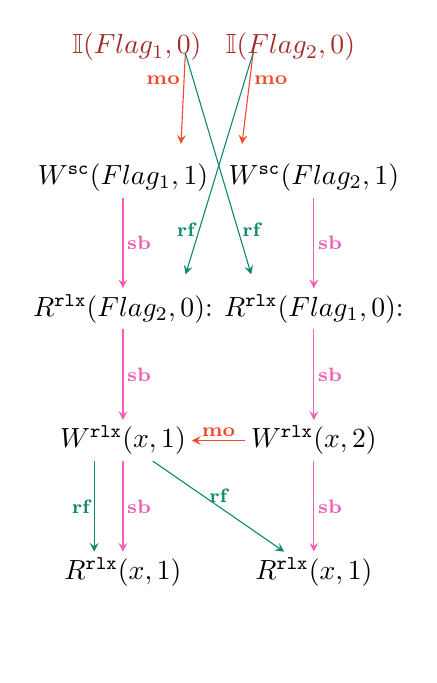
\begin{tikzpicture}[x=1em,y=1em,yscale=-1,xscale=-1]
	\tikzstyle{every node}=[font=\normalfont]
	
	\node (ifl1) [inner sep=2pt,color=Brown] {$\mathbb{I}(Flag_1,0)$};
	\node (ifl2) [right=30pt,inner sep=2pt,color=Brown] {$\mathbb{I}(Flag_2,0)$};
	
	\node (f11) [below left=10pt and -30pt of ifl1,inner sep=2pt, color=White] {$\mathbb{F}_{11}$};
	\node (fl1) [below=10pt of f11, inner sep=2pt] {$ W^\sc(Flag_1,1) $};
	\node (f12) [below=10pt of fl1, inner sep=2pt, color=White] {$\mathbb{F}_{12}$};
	\node (rfl2) [below=10pt of f12, inner sep=2pt] {$R^\rlx(Flag_2,0)$:};
	\node (f13) [below=10pt of rfl2, inner sep=2pt, color=White] {$\mathbb{F}_{13}$};
	\node (cs11) [below=10pt of f13, inner sep=2pt] {$ W^\rlx(x,1) $};
	\node (f14) [below=10pt of cs11, inner sep=2pt, color=White] {$\mathbb{F}_{14}$};
	\node (cs12) [below=10pt of f14, inner sep=2pt] {$ R^\rlx(x,1) $};
	\node (f15) [below=10pt of cs12, inner sep=2pt, color=White] {$\mathbb{F}_{15}$};
	
	\node (f21) [right=50pt of f11, inner sep=2pt, color=White] {$\mathbb{F}_{21}$};
	\node (fl2) [below=10pt of f21, inner sep=2pt] {$W^\sc(Flag_2,1)$};
	\node (f22) [below=10pt of fl2, inner sep=2pt, color=White] {$\mathbb{F}_{22}$};
	\node (rfl1) [below=10pt of f22, inner sep=2pt] {$R^\rlx(Flag_1,0)$:};
	\node (f23) [below=10pt of rfl1, inner sep=2pt, color=White] {$\mathbb{F}_{23}$};
	\node (cs21) [below=10pt of f23, inner sep=2pt] {$ W^\rlx(x,2) $};
	\node (f24) [below=10pt of cs21, inner sep=2pt, color=White] {$\mathbb{F}_{24}$};
	\node (cs22) [below=10pt of f24, inner sep=2pt] {$ R^\rlx(x,1) $};
	\node (f25) [below=10pt of cs22, inner sep=2pt, color=White] {$\mathbb{F}_{23}$};
	%
	\draw [->,>=stealth,color=RedOrange] ($ (ifl1.south east)+(0.8,-5pt) $) -- node[pos=0.3,left=-2pt,font=\scriptsize,color=black] { $\lmo$ } ($ (fl1.north east)+(1.2,-5pt) $);
	\draw [->,>=stealth,color=RedOrange] ($ (ifl2.south west)+(-1.2,-5pt) $) -- node[pos=0.3,right=-2pt,font=\scriptsize,color=black] { $\lmo$ } ($ (fl2.north west)+(-0.7,-5pt) $);
	
	\draw [->,>=stealth,color=PineGreen] ($ (ifl1.south east)+(0.8,-5pt) $) -- node[pos=0.8,right=-2pt,font=\scriptsize,color=black] { $\lrf$ } ($ (rfl1.north west)+(-1.2,-5pt) $);
	\draw [->,>=stealth,color=PineGreen] ($ (ifl2.south west)+(-1.2,-5pt) $) -- node[pos=0.8,left=-2pt,font=\scriptsize,color=black] { $\lrf$ } ($ (rfl2.north east)+(1.2,-5pt) $);
	
	\draw [->,>=stealth,color=RedOrange] (cs21)  -- node[midway,above=-2pt,font=\scriptsize,color=black] { $\lmo$ } (cs11);
	\draw [->,>=stealth,color=PineGreen] (cs11)  -- node[midway,above=-2pt,font=\scriptsize,color=black] { $\lrf$ } (cs22);
	\draw [->,>=stealth,color=PineGreen] ($ (cs11.south)+(10.4pt,0) $)  -- node[midway,left=-2pt,font=\scriptsize,color=black] { $\lrf$ } ($ (cs12.north)+(10.4pt,0) $);
	
	\draw [->,>=stealth,color=CarnationPink] (fl1)  -- node[midway,right=-2pt,font=\scriptsize,color=black] { $\lsb$ } (rfl2);
	\draw [->,>=stealth,color=CarnationPink] (rfl2) -- node[midway,right=-2pt,font=\scriptsize,color=black] { $\lsb$ } (cs11);
	\draw [->,>=stealth,color=CarnationPink] (cs11) -- node[midway,right=-2pt,font=\scriptsize,color=black] { $\lsb$ } (cs12);
	
	\draw [->,>=stealth,color=CarnationPink] (fl2)  -- node[midway,right=-2pt,font=\scriptsize,color=black] { $\lsb$ } (rfl1);
	\draw [->,>=stealth,color=CarnationPink] (rfl1) -- node[midway,right=-2pt,font=\scriptsize,color=black] { $\lsb$ } (cs21);
	\draw [->,>=stealth,color=CarnationPink] (cs21) -- node[midway,right=-2pt,font=\scriptsize,color=black] { $\lsb$ } (cs22);
	
\end{tikzpicture}
} &
		\resizebox{0.24\textwidth}{!}{\tikzset{every picture/.style={line width=0.75pt}} %set default line width to 0.75pt        
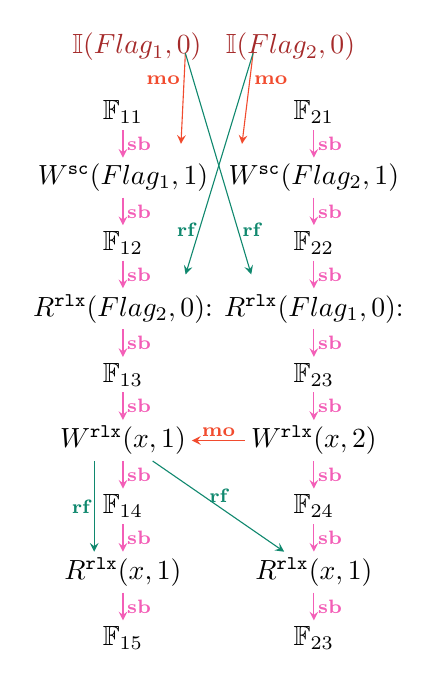
\begin{tikzpicture}[x=1em,y=1em,yscale=-1,xscale=-1]
	\tikzstyle{every node}=[font=\normalfont]
	
	\node (ifl1) [inner sep=2pt,color=Brown] {$\mathbb{I}(Flag_1,0)$};
	\node (ifl2) [right=30pt,inner sep=2pt,color=Brown] {$\mathbb{I}(Flag_2,0)$};
	
	\node (f11) [below left=10pt and -30pt of ifl1,inner sep=2pt] {$\mathbb{F}_{11}$};
	\node (fl1) [below=10pt of f11, inner sep=2pt] {$ W^\sc(Flag_1,1) $};
	\node (f12) [below=10pt of fl1, inner sep=2pt] {$\mathbb{F}_{12}$};
	\node (rfl2) [below=10pt of f12, inner sep=2pt] {$R^\rlx(Flag_2,0)$:};
	\node (f13) [below=10pt of rfl2, inner sep=2pt] {$\mathbb{F}_{13}$};
	\node (cs11) [below=10pt of f13, inner sep=2pt] {$ W^\rlx(x,1) $};
	\node (f14) [below=10pt of cs11, inner sep=2pt] {$\mathbb{F}_{14}$};
	\node (cs12) [below=10pt of f14, inner sep=2pt] {$ R^\rlx(x,1) $};
	\node (f15) [below=10pt of cs12, inner sep=2pt] {$\mathbb{F}_{15}$};
	
	\node (f21) [right=50pt of f11, inner sep=2pt] {$\mathbb{F}_{21}$};
	\node (fl2) [below=10pt of f21, inner sep=2pt] {$W^\sc(Flag_2,1)$};
	\node (f22) [below=10pt of fl2, inner sep=2pt] {$\mathbb{F}_{22}$};
	\node (rfl1) [below=10pt of f22, inner sep=2pt] {$R^\rlx(Flag_1,0)$:};
	\node (f23) [below=10pt of rfl1, inner sep=2pt] {$\mathbb{F}_{23}$};
	\node (cs21) [below=10pt of f23, inner sep=2pt] {$ W^\rlx(x,2) $};
	\node (f24) [below=10pt of cs21, inner sep=2pt] {$\mathbb{F}_{24}$};
	\node (cs22) [below=10pt of f24, inner sep=2pt] {$ R^\rlx(x,1) $};
	\node (f25) [below=10pt of cs22, inner sep=2pt] {$\mathbb{F}_{23}$};
	%
	\draw [->,>=stealth,color=RedOrange] ($ (ifl1.south east)+(0.8,-5pt) $) -- node[pos=0.3,left=-2pt,font=\scriptsize,color=black] { $\lmo$ } ($ (fl1.north east)+(1.2,-5pt) $);
	\draw [->,>=stealth,color=RedOrange] ($ (ifl2.south west)+(-1.2,-5pt) $) -- node[pos=0.3,right=-2pt,font=\scriptsize,color=black] { $\lmo$ } ($ (fl2.north west)+(-0.7,-5pt) $);
	
	\draw [->,>=stealth,color=PineGreen] ($ (ifl1.south east)+(0.8,-5pt) $) -- node[pos=0.8,right=-2pt,font=\scriptsize,color=black] { $\lrf$ } ($ (rfl1.north west)+(-1.2,-5pt) $);
	\draw [->,>=stealth,color=PineGreen] ($ (ifl2.south west)+(-1.2,-5pt) $) -- node[pos=0.8,left=-2pt,font=\scriptsize,color=black] { $\lrf$ } ($ (rfl2.north east)+(1.2,-5pt) $);
	
	\draw [->,>=stealth,color=RedOrange] (cs21)  -- node[midway,above=-2pt,font=\scriptsize,color=black] { $\lmo$ } (cs11);
	\draw [->,>=stealth,color=PineGreen] (cs11)  -- node[midway,above=-2pt,font=\scriptsize,color=black] { $\lrf$ } (cs22);
	\draw [->,>=stealth,color=PineGreen] ($ (cs11.south)+(10.4pt,0) $)  -- node[midway,left=-2pt,font=\scriptsize,color=black] { $\lrf$ } ($ (cs12.north)+(10.4pt,0) $);
	
	\draw [->,>=stealth,color=CarnationPink] (f11)  -- node[midway,right=-2pt,font=\scriptsize,color=black] { $\lsb$ } (fl1);
	\draw [->,>=stealth,color=CarnationPink] (fl1)  -- node[midway,right=-2pt,font=\scriptsize,color=black] { $\lsb$ } (f12);
	\draw [->,>=stealth,color=CarnationPink] (f12)  -- node[midway,right=-2pt,font=\scriptsize,color=black] { $\lsb$ } (rfl2);
	\draw [->,>=stealth,color=CarnationPink] (rfl2) -- node[midway,right=-2pt,font=\scriptsize,color=black] { $\lsb$ } (f13);
	\draw [->,>=stealth,color=CarnationPink] (f13)  -- node[midway,right=-2pt,font=\scriptsize,color=black] { $\lsb$ } (cs11);
	\draw [->,>=stealth,color=CarnationPink] (cs11) -- node[midway,right=-2pt,font=\scriptsize,color=black] { $\lsb$ } (f14);
	\draw [->,>=stealth,color=CarnationPink] (f14)  -- node[midway,right=-2pt,font=\scriptsize,color=black] { $\lsb$ } (cs12);
	\draw [->,>=stealth,color=CarnationPink] (cs12) -- node[midway,right=-2pt,font=\scriptsize,color=black] { $\lsb$ } (f15);
	
	\draw [->,>=stealth,color=CarnationPink] (f21)  -- node[midway,right=-2pt,font=\scriptsize,color=black] { $\lsb$ } (fl2);
	\draw [->,>=stealth,color=CarnationPink] (fl2)  -- node[midway,right=-2pt,font=\scriptsize,color=black] { $\lsb$ } (f22);
	\draw [->,>=stealth,color=CarnationPink] (f22)  -- node[midway,right=-2pt,font=\scriptsize,color=black] { $\lsb$ } (rfl1);
	\draw [->,>=stealth,color=CarnationPink] (rfl1) -- node[midway,right=-2pt,font=\scriptsize,color=black] { $\lsb$ } (f23);
	\draw [->,>=stealth,color=CarnationPink] (f23)  -- node[midway,right=-2pt,font=\scriptsize,color=black] { $\lsb$ } (cs21);
	\draw [->,>=stealth,color=CarnationPink] (cs21) -- node[midway,right=-2pt,font=\scriptsize,color=black] { $\lsb$ } (f24);
	\draw [->,>=stealth,color=CarnationPink] (f24)  -- node[midway,right=-2pt,font=\scriptsize,color=black] { $\lsb$ } (cs22);
	\draw [->,>=stealth,color=CarnationPink] (cs22) -- node[midway,right=-2pt,font=\scriptsize,color=black] { $\lsb$ } (f25);
	
\end{tikzpicture}
} &
		\resizebox{0.24\textwidth}{!}{\tikzset{every picture/.style={line width=0.75pt}} %set default line width to 0.75pt        
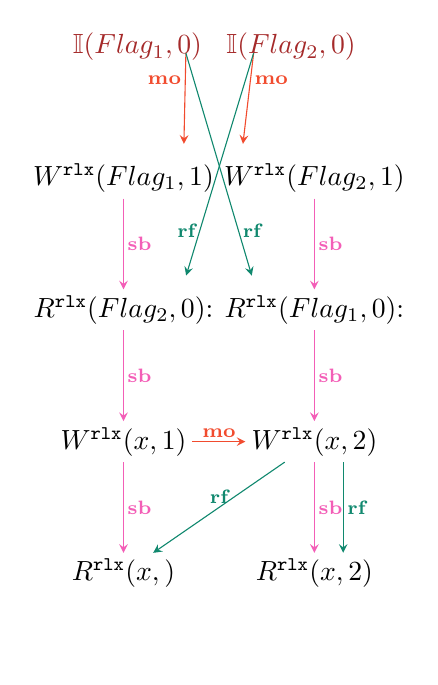
\begin{tikzpicture}[x=1em,y=1em,yscale=-1,xscale=-1]
	\tikzstyle{every node}=[font=\normalfont]
	
	\node (ifl1) [inner sep=2pt,color=Brown] {$\mathbb{I}(Flag_1,0)$};
	\node (ifl2) [right=30pt,inner sep=2pt,color=Brown] {$\mathbb{I}(Flag_2,0)$};
	
	\node (f11) [below left=10pt and -30pt of ifl1,inner sep=2pt, color=White] {$\mathbb{F}_{11}$};
	\node (fl1) [below=10pt of f11, inner sep=2pt] {$ W^\rlx(Flag_1,1) $};
	\node (f12) [below=10pt of fl1, inner sep=2pt, color=White] {$\mathbb{F}_{12}$};
	\node (rfl2) [below=10pt of f12, inner sep=2pt] {$R^\rlx(Flag_2,0)$:};
	\node (f13) [below=10pt of rfl2, inner sep=2pt, color=White] {$\mathbb{F}_{13}$};
	\node (cs11) [below=10pt of f13, inner sep=2pt] {$ W^\rlx(x,1) $};
	\node (f14) [below=10pt of cs11, inner sep=2pt, color=White] {$\mathbb{F}_{14}$};
	\node (cs12) [below=10pt of f14, inner sep=2pt] {$ R^\rlx(x,) $};
	\node (f15) [below=10pt of cs12, inner sep=2pt, color=White] {$\mathbb{F}_{15}$};
	
	\node (f21) [right=50pt of f11, inner sep=2pt, color=White] {$\mathbb{F}_{21}$};
	\node (fl2) [below=10pt of f21, inner sep=2pt] {$W^\rlx(Flag_2,1)$};
	\node (f22) [below=10pt of fl2, inner sep=2pt, color=White] {$\mathbb{F}_{22}$};
	\node (rfl1) [below=10pt of f22, inner sep=2pt] {$R^\rlx(Flag_1,0)$:};
	\node (f23) [below=10pt of rfl1, inner sep=2pt, color=White] {$\mathbb{F}_{23}$};
	\node (cs21) [below=10pt of f23, inner sep=2pt] {$ W^\rlx(x,2) $};
	\node (f24) [below=10pt of cs21, inner sep=2pt, color=White] {$\mathbb{F}_{24}$};
	\node (cs22) [below=10pt of f24, inner sep=2pt] {$ R^\rlx(x,2) $};
	\node (f25) [below=10pt of cs22, inner sep=2pt, color=White] {$\mathbb{F}_{23}$};
	%
	\draw [->,>=stealth,color=RedOrange] ($ (ifl1.south east)+(0.8,-5pt) $) -- node[pos=0.3,left=-2pt,font=\scriptsize,color=black] { $\lmo$ } ($ (fl1.north east)+(1.3,-5pt) $);
	\draw [->,>=stealth,color=RedOrange] ($ (ifl2.south west)+(-1.2,-5pt) $) -- node[pos=0.3,right=-2pt,font=\scriptsize,color=black] { $\lmo$ } ($ (fl2.north west)+(-0.9,-5pt) $);
	
	\draw [->,>=stealth,color=PineGreen] ($ (ifl1.south east)+(0.8,-5pt) $) -- node[pos=0.8,right=-2pt,font=\scriptsize,color=black] { $\lrf$ } ($ (rfl1.north west)+(-1.2,-5pt) $);
	\draw [->,>=stealth,color=PineGreen] ($ (ifl2.south west)+(-1.2,-5pt) $) -- node[pos=0.8,left=-2pt,font=\scriptsize,color=black] { $\lrf$ } ($ (rfl2.north east)+(1.2,-5pt) $);
	
	\draw [->,>=stealth,color=RedOrange] (cs11)  -- node[midway,above=-2pt,font=\scriptsize,color=black] { $\lmo$ } (cs21);
	\draw [->,>=stealth,color=PineGreen] (cs21)  -- node[midway,above=-2pt,font=\scriptsize,color=black] { $\lrf$ } (cs12);
	\draw [->,>=stealth,color=PineGreen] ($ (cs21.south)+(-10.4pt,0) $)  -- node[midway,right=-2pt,font=\scriptsize,color=black] { $\lrf$ } ($ (cs22.north)+(-10.4pt,0) $);
	
	\draw [->,>=stealth,color=CarnationPink] (fl1)  -- node[midway,right=-2pt,font=\scriptsize,color=black] { $\lsb$ } (rfl2);
	\draw [->,>=stealth,color=CarnationPink] (rfl2) -- node[midway,right=-2pt,font=\scriptsize,color=black] { $\lsb$ } (cs11);
	\draw [->,>=stealth,color=CarnationPink] (cs11) -- node[midway,right=-2pt,font=\scriptsize,color=black] { $\lsb$ } (cs12);
	
	\draw [->,>=stealth,color=CarnationPink] (fl2)  -- node[midway,right=-2pt,font=\scriptsize,color=black] { $\lsb$ } (rfl1);
	\draw [->,>=stealth,color=CarnationPink] (rfl1) -- node[midway,right=-2pt,font=\scriptsize,color=black] { $\lsb$ } (cs21);
	\draw [->,>=stealth,color=CarnationPink] (cs21) -- node[midway,right=-2pt,font=\scriptsize,color=black] { $\lsb$ } (cs22);
	
\end{tikzpicture}
} &
		\resizebox{0.24\textwidth}{!}{\tikzset{every picture/.style={line width=0.75pt}} %set default line width to 0.75pt        
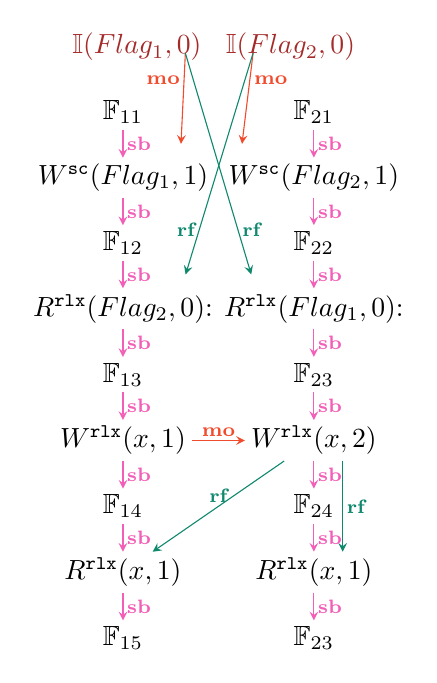
\begin{tikzpicture}[x=1em,y=1em,yscale=-1,xscale=-1]
	\tikzstyle{every node}=[font=\normalfont]
	
	\node (ifl1) [inner sep=2pt,color=Brown] {$\mathbb{I}(Flag_1,0)$};
	\node (ifl2) [right=30pt,inner sep=2pt,color=Brown] {$\mathbb{I}(Flag_2,0)$};
	
	\node (f11) [below left=10pt and -30pt of ifl1,inner sep=2pt] {$\mathbb{F}_{11}$};
	\node (fl1) [below=10pt of f11, inner sep=2pt] {$ W^\sc(Flag_1,1) $};
	\node (f12) [below=10pt of fl1, inner sep=2pt] {$\mathbb{F}_{12}$};
	\node (rfl2) [below=10pt of f12, inner sep=2pt] {$R^\rlx(Flag_2,0)$:};
	\node (f13) [below=10pt of rfl2, inner sep=2pt] {$\mathbb{F}_{13}$};
	\node (cs11) [below=10pt of f13, inner sep=2pt] {$ W^\rlx(x,1) $};
	\node (f14) [below=10pt of cs11, inner sep=2pt] {$\mathbb{F}_{14}$};
	\node (cs12) [below=10pt of f14, inner sep=2pt] {$ R^\rlx(x,1) $};
	\node (f15) [below=10pt of cs12, inner sep=2pt] {$\mathbb{F}_{15}$};
	
	\node (f21) [right=50pt of f11, inner sep=2pt] {$\mathbb{F}_{21}$};
	\node (fl2) [below=10pt of f21, inner sep=2pt] {$W^\sc(Flag_2,1)$};
	\node (f22) [below=10pt of fl2, inner sep=2pt] {$\mathbb{F}_{22}$};
	\node (rfl1) [below=10pt of f22, inner sep=2pt] {$R^\rlx(Flag_1,0)$:};
	\node (f23) [below=10pt of rfl1, inner sep=2pt] {$\mathbb{F}_{23}$};
	\node (cs21) [below=10pt of f23, inner sep=2pt] {$ W^\rlx(x,2) $};
	\node (f24) [below=10pt of cs21, inner sep=2pt] {$\mathbb{F}_{24}$};
	\node (cs22) [below=10pt of f24, inner sep=2pt] {$ R^\rlx(x,1) $};
	\node (f25) [below=10pt of cs22, inner sep=2pt] {$\mathbb{F}_{23}$};
	%
	\draw [->,>=stealth,color=RedOrange] ($ (ifl1.south east)+(0.8,-5pt) $) -- node[pos=0.3,left=-2pt,font=\scriptsize,color=black] { $\lmo$ } ($ (fl1.north east)+(1.2,-5pt) $);
	\draw [->,>=stealth,color=RedOrange] ($ (ifl2.south west)+(-1.2,-5pt) $) -- node[pos=0.3,right=-2pt,font=\scriptsize,color=black] { $\lmo$ } ($ (fl2.north west)+(-0.7,-5pt) $);
	
	\draw [->,>=stealth,color=PineGreen] ($ (ifl1.south east)+(0.8,-5pt) $) -- node[pos=0.8,right=-2pt,font=\scriptsize,color=black] { $\lrf$ } ($ (rfl1.north west)+(-1.2,-5pt) $);
	\draw [->,>=stealth,color=PineGreen] ($ (ifl2.south west)+(-1.2,-5pt) $) -- node[pos=0.8,left=-2pt,font=\scriptsize,color=black] { $\lrf$ } ($ (rfl2.north east)+(1.2,-5pt) $);
	
	\draw [->,>=stealth,color=RedOrange] (cs11)  -- node[midway,above=-2pt,font=\scriptsize,color=black] { $\lmo$ } (cs21);
	\draw [->,>=stealth,color=PineGreen] (cs21)  -- node[midway,above=-2pt,font=\scriptsize,color=black] { $\lrf$ } (cs12);
	\draw [->,>=stealth,color=PineGreen] ($ (cs21.south)+(-10.4pt,0) $)  -- node[midway,right=-2pt,font=\scriptsize,color=black] { $\lrf$ } ($ (cs22.north)+(-10.4pt,0) $);
	
	\draw [->,>=stealth,color=CarnationPink] (f11)  -- node[midway,right=-2pt,font=\scriptsize,color=black] { $\lsb$ } (fl1);
	\draw [->,>=stealth,color=CarnationPink] (fl1)  -- node[midway,right=-2pt,font=\scriptsize,color=black] { $\lsb$ } (f12);
	\draw [->,>=stealth,color=CarnationPink] (f12)  -- node[midway,right=-2pt,font=\scriptsize,color=black] { $\lsb$ } (rfl2);
	\draw [->,>=stealth,color=CarnationPink] (rfl2) -- node[midway,right=-2pt,font=\scriptsize,color=black] { $\lsb$ } (f13);
	\draw [->,>=stealth,color=CarnationPink] (f13)  -- node[midway,right=-2pt,font=\scriptsize,color=black] { $\lsb$ } (cs11);
	\draw [->,>=stealth,color=CarnationPink] (cs11) -- node[midway,right=-2pt,font=\scriptsize,color=black] { $\lsb$ } (f14);
	\draw [->,>=stealth,color=CarnationPink] (f14)  -- node[midway,right=-2pt,font=\scriptsize,color=black] { $\lsb$ } (cs12);
	\draw [->,>=stealth,color=CarnationPink] (cs12) -- node[midway,right=-2pt,font=\scriptsize,color=black] { $\lsb$ } (f15);
	
	\draw [->,>=stealth,color=CarnationPink] (f21)  -- node[midway,right=-2pt,font=\scriptsize,color=black] { $\lsb$ } (fl2);
	\draw [->,>=stealth,color=CarnationPink] (fl2)  -- node[midway,right=-2pt,font=\scriptsize,color=black] { $\lsb$ } (f22);
	\draw [->,>=stealth,color=CarnationPink] (f22)  -- node[midway,right=-2pt,font=\scriptsize,color=black] { $\lsb$ } (rfl1);
	\draw [->,>=stealth,color=CarnationPink] (rfl1) -- node[midway,right=-2pt,font=\scriptsize,color=black] { $\lsb$ } (f23);
	\draw [->,>=stealth,color=CarnationPink] (f23)  -- node[midway,right=-2pt,font=\scriptsize,color=black] { $\lsb$ } (cs21);
	\draw [->,>=stealth,color=CarnationPink] (cs21) -- node[midway,right=-2pt,font=\scriptsize,color=black] { $\lsb$ } (f24);
	\draw [->,>=stealth,color=CarnationPink] (f24)  -- node[midway,right=-2pt,font=\scriptsize,color=black] { $\lsb$ } (cs22);
	\draw [->,>=stealth,color=CarnationPink] (cs22) -- node[midway,right=-2pt,font=\scriptsize,color=black] { $\lsb$ } (f25);
	
\end{tikzpicture}
} \\
		\hline
		
		\multicolumn{1}{c}{\hl{mutex-bt1}} &
		\multicolumn{1}{c}{$\imm{\hl{mutex-bt1}}$}  &
		\multicolumn{1}{c}{\hl{mutex-bt2}} &
		\multicolumn{1}{c}{$\imm{\hl{mutex-bt2}}$} \\
		
		\multicolumn{1}{c}{buggy trace 1} &
		\multicolumn{1}{c}{intermediate} &
		\multicolumn{1}{c}{buggy trace 2} &
		\multicolumn{1}{c}{intermediate} \\
	
		\multicolumn{1}{c}{} &
		\multicolumn{1}{c}{buggy trace 1} &
		\multicolumn{1}{c}{} &
		\multicolumn{1}{c}{buggy trace 2} \\
	\end{tabular}
\end{figure}

Algorithm~\ref{alg:main algo} iterates over each buggy trace
$\tau$ (line 4) and transforms the trace to an intermediate 
trace $\imm{\tau}$ (line 5). The algorithm further updates the 
event relations accordingly (line 6). As discussed in Section
\ref{sec:invalidating ce} a change is witnessed in the 
$\setHB$ relation. The transformed intermediate traces 
corresponding to buggy traces \hlref{mutex-bt1} and 
\hlref{mutex-bt2}, along with the updated event relations are 
represented in $\imm{\hlref{mutex-bt1}}$ and 
$\imm{\hlref{mutex-bt2}}$ respectively.

\noindent
{\bf Detecting cyclic relations indicating violation of 
	trace coherence}
In each intermediate buggy trace, the algorithm proceeds 
to perform \wkfence (line 7) and return cycles in compositions 
of event relations that define a coherence condition 
(Section~\ref{sec:c11}). For the intermediate traces 
$\imm{\hlref{mutex-bt1}}$ and $\imm{\hlref{mutex-bt2}}$
\wkfence would return an empty set.
%
The algorithm then proceeds to perform \stfence (line 8) that 
computes the $\so{\imm{\tau}}{}{}$ relation on \sc 
events and returns the cycles in $\so{\imm{\tau}}{}{}$.
The cyclic $\so{\imm{\tau}}{}{}$ relations in the intermediate
traces $\imm{\hlref{mutex-bt1}}$ and $\imm{\hlref{mutex-bt2}}$
are shown in $\imm{\hlref{mutex-bt1-so}}$ and 
$\imm{\hlref{mutex-bt2-so}}$. Note that, $\so{\imm{\tau}}{}{}$ 
would also be formed between every fence before 
$\mathbb{F}^\sc_{13}$ and every fence including and after 
$\mathbb{F}^\sc_{24}$ in $\imm{\hlref{mutex-bt1-so}}$ 
(correspondingly in $\imm{\hlref{mutex-bt1-so}}$), however, we 
have skipped the edges in the figures for better readability.

\begin{figure}[!h]
	\begin{tabular}{|c|c|}
		\hline
		\resizebox{0.24\textwidth}{!}{\tikzset{every picture/.style={line width=0.75pt}} %set default line width to 0.75pt        
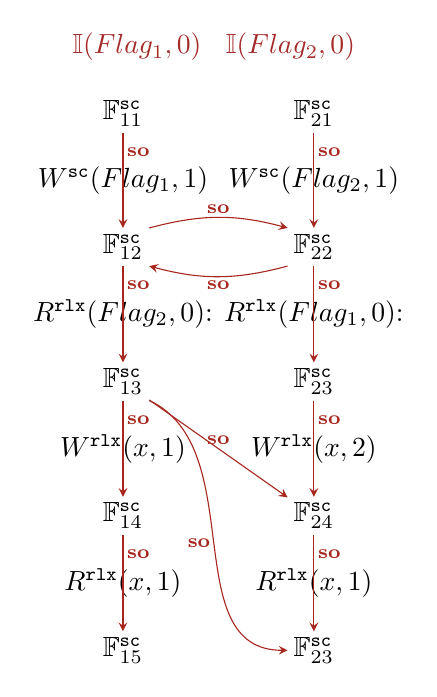
\begin{tikzpicture}[x=1em,y=1em,yscale=-1,xscale=-1]
	\tikzstyle{every node}=[font=\normalfont]
	
	\node (ifl1) [inner sep=2pt,color=Brown] {$\mathbb{I}(Flag_1,0)$};
	\node (ifl2) [right=30pt,inner sep=2pt,color=Brown] {$\mathbb{I}(Flag_2,0)$};
	
	\node (f11) [below left=10pt and -30pt of ifl1,inner sep=2pt] {$\mathbb{F}^\sc_{11}$};
	\node (fl1) [below=10pt of f11, inner sep=2pt] {$ W^\sc(Flag_1,1) $};
	\node (f12) [below=10pt of fl1, inner sep=2pt] {$\mathbb{F}^\sc_{12}$};
	\node (rfl2) [below=10pt of f12, inner sep=2pt] {$R^\rlx(Flag_2,0)$:};
	\node (f13) [below=10pt of rfl2, inner sep=2pt] {$\mathbb{F}^\sc_{13}$};
	\node (cs11) [below=10pt of f13, inner sep=2pt] {$ W^\rlx(x,1) $};
	\node (f14) [below=10pt of cs11, inner sep=2pt] {$\mathbb{F}^\sc_{14}$};
	\node (cs12) [below=10pt of f14, inner sep=2pt] {$ R^\rlx(x,1) $};
	\node (f15) [below=10pt of cs12, inner sep=2pt] {$\mathbb{F}^\sc_{15}$};
	
	\node (f21) [right=50pt of f11, inner sep=2pt] {$\mathbb{F}^\sc_{21}$};
	\node (fl2) [below=10pt of f21, inner sep=2pt] {$W^\sc(Flag_2,1)$};
	\node (f22) [below=10pt of fl2, inner sep=2pt] {$\mathbb{F}^\sc_{22}$};
	\node (rfl1) [below=10pt of f22, inner sep=2pt] {$R^\rlx(Flag_1,0)$:};
	\node (f23) [below=10pt of rfl1, inner sep=2pt] {$\mathbb{F}^\sc_{23}$};
	\node (cs21) [below=10pt of f23, inner sep=2pt] {$ W^\rlx(x,2) $};
	\node (f24) [below=10pt of cs21, inner sep=2pt] {$\mathbb{F}^\sc_{24}$};
	\node (cs22) [below=10pt of f24, inner sep=2pt] {$ R^\rlx(x,1) $};
	\node (f25) [below=10pt of cs22, inner sep=2pt] {$\mathbb{F}^\sc_{23}$};
	%
	
	\draw [->,>=stealth,color=Mahogany] (f11)  -- node[pos=0.2,right=-2pt,font=\scriptsize,color=black] { $\lso$ } (f12);
	\draw [->,>=stealth,color=Mahogany] (f12)  -- node[pos=0.2,right=-2pt,font=\scriptsize,color=black] { $\lso$ } (f13);
	\draw [->,>=stealth,color=Mahogany] (f13)  -- node[pos=0.2,right=-2pt,font=\scriptsize,color=black] { $\lso$ } (f14);
	\draw [->,>=stealth,color=Mahogany] (f14)  -- node[pos=0.2,right=-2pt,font=\scriptsize,color=black] { $\lso$ } (f15);
	
	\draw [->,>=stealth,color=Mahogany] (f21)  -- node[pos=0.2,right=-2pt,font=\scriptsize,color=black] { $\lso$ } (f22);
	\draw [->,>=stealth,color=Mahogany] (f22)  -- node[pos=0.2,right=-2pt,font=\scriptsize,color=black] { $\lso$ } (f23);
	\draw [->,>=stealth,color=Mahogany] (f23)  -- node[pos=0.2,right=-2pt,font=\scriptsize,color=black] { $\lso$ } (f24);
	\draw [->,>=stealth,color=Mahogany] (f24)  -- node[pos=0.2,right=-2pt,font=\scriptsize,color=black] { $\lso$ } (f25);
	
	\draw [->,>=stealth,color=Mahogany] ($ (f12.north east) $)  to[out=-165,in=-15] node[midway,above=-2pt,font=\scriptsize,color=black] { $\lso$ } ($ (f22.north west) $);
	\draw [->,>=stealth,color=Mahogany] ($(f22.south west)$)  to[out=15,in=165] node[midway,below=-2pt,font=\scriptsize,color=black] { $\lso$ } ($(f12.south east)$);
	
	\draw [->,>=stealth,color=Mahogany] (f13)  -- node[midway,above=-2pt,font=\scriptsize,color=black] { $\lso$ } (f24);
	\draw [->,>=stealth,color=Mahogany] ($(f13.south east)$)  to[out=155,in=0] node[midway,left=-2pt,font=\scriptsize,color=black] { $\lso$ } ($(f25.west)$);
	
\end{tikzpicture}
} &
		\resizebox{0.24\textwidth}{!}{\tikzset{every picture/.style={line width=0.75pt}} %set default line width to 0.75pt        
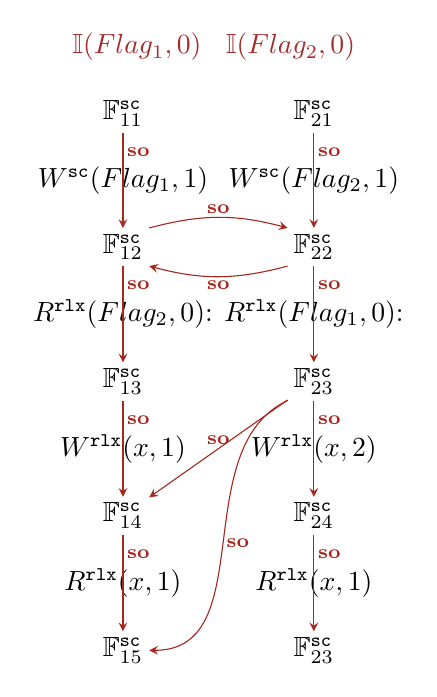
\begin{tikzpicture}[x=1em,y=1em,yscale=-1,xscale=-1]
	\tikzstyle{every node}=[font=\normalfont]
	
	\node (ifl1) [inner sep=2pt,color=Brown] {$\mathbb{I}(Flag_1,0)$};
	\node (ifl2) [right=30pt,inner sep=2pt,color=Brown] {$\mathbb{I}(Flag_2,0)$};
	
	\node (f11) [below left=10pt and -30pt of ifl1,inner sep=2pt] {$\mathbb{F}^\sc_{11}$};
	\node (fl1) [below=10pt of f11, inner sep=2pt] {$ W^\sc(Flag_1,1) $};
	\node (f12) [below=10pt of fl1, inner sep=2pt] {$\mathbb{F}^\sc_{12}$};
	\node (rfl2) [below=10pt of f12, inner sep=2pt] {$R^\rlx(Flag_2,0)$:};
	\node (f13) [below=10pt of rfl2, inner sep=2pt] {$\mathbb{F}^\sc_{13}$};
	\node (cs11) [below=10pt of f13, inner sep=2pt] {$ W^\rlx(x,1) $};
	\node (f14) [below=10pt of cs11, inner sep=2pt] {$\mathbb{F}^\sc_{14}$};
	\node (cs12) [below=10pt of f14, inner sep=2pt] {$ R^\rlx(x,1) $};
	\node (f15) [below=10pt of cs12, inner sep=2pt] {$\mathbb{F}^\sc_{15}$};
	
	\node (f21) [right=50pt of f11, inner sep=2pt] {$\mathbb{F}^\sc_{21}$};
	\node (fl2) [below=10pt of f21, inner sep=2pt] {$W^\sc(Flag_2,1)$};
	\node (f22) [below=10pt of fl2, inner sep=2pt] {$\mathbb{F}^\sc_{22}$};
	\node (rfl1) [below=10pt of f22, inner sep=2pt] {$R^\rlx(Flag_1,0)$:};
	\node (f23) [below=10pt of rfl1, inner sep=2pt] {$\mathbb{F}^\sc_{23}$};
	\node (cs21) [below=10pt of f23, inner sep=2pt] {$ W^\rlx(x,2) $};
	\node (f24) [below=10pt of cs21, inner sep=2pt] {$\mathbb{F}^\sc_{24}$};
	\node (cs22) [below=10pt of f24, inner sep=2pt] {$ R^\rlx(x,1) $};
	\node (f25) [below=10pt of cs22, inner sep=2pt] {$\mathbb{F}^\sc_{23}$};
	%
	
	\draw [->,>=stealth,color=Mahogany] (f11)  -- node[pos=0.2,right=-2pt,font=\scriptsize,color=black] { $\lso$ } (f12);
	\draw [->,>=stealth,color=Mahogany] (f12)  -- node[pos=0.2,right=-2pt,font=\scriptsize,color=black] { $\lso$ } (f13);
	\draw [->,>=stealth,color=Mahogany] (f13)  -- node[pos=0.2,right=-2pt,font=\scriptsize,color=black] { $\lso$ } (f14);
	\draw [->,>=stealth,color=Mahogany] (f14)  -- node[pos=0.2,right=-2pt,font=\scriptsize,color=black] { $\lso$ } (f15);
	
	\draw [->,>=stealth,color=Mahogany] (f21)  -- node[pos=0.2,right=-2pt,font=\scriptsize,color=black] { $\lso$ } (f22);
	\draw [->,>=stealth,color=Mahogany] (f22)  -- node[pos=0.2,right=-2pt,font=\scriptsize,color=black] { $\lso$ } (f23);
	\draw [->,>=stealth,color=Mahogany] (f23)  -- node[pos=0.2,right=-2pt,font=\scriptsize,color=black] { $\lso$ } (f24);
	\draw [->,>=stealth,color=Mahogany] (f24)  -- node[pos=0.2,right=-2pt,font=\scriptsize,color=black] { $\lso$ } (f25);
	
	\draw [->,>=stealth,color=Mahogany] ($ (f12.north east) $)  to[out=-165,in=-15] node[midway,above=-2pt,font=\scriptsize,color=black] { $\lso$ } ($ (f22.north west) $);
	\draw [->,>=stealth,color=Mahogany] ($(f22.south west)$)  to[out=15,in=165] node[midway,below=-2pt,font=\scriptsize,color=black] { $\lso$ } ($(f12.south east)$);
	
	\draw [->,>=stealth,color=Mahogany] (f23)  -- node[midway,above=-2pt,font=\scriptsize,color=black] { $\lso$ } (f14);
	\draw [->,>=stealth,color=Mahogany] ($(f23.south west)$)  to[out=25,in=180] node[midway,right=-2pt,font=\scriptsize,color=black] { $\lso$ } ($(f15.east)$);
	
\end{tikzpicture}
} \\
		\hline
		
		\multicolumn{1}{c}{$\imm{\hl{mutex-bt1-so}}$}  &
		\multicolumn{1}{c}{$\imm{\hl{mutex-bt2-so}}$-} \\
		
		\multicolumn{1}{c}{intermediate} &
		\multicolumn{1}{c}{intermediate} \\
		
		\multicolumn{1}{c}{buggy trace 1} &
		\multicolumn{1}{c}{buggy trace 2} \\
	\end{tabular}
\end{figure}


\subsection{Reducing Fence Synthesis to SAT problem}
Recall that transitive closure of $ \so{\imm{\tau}}{}{} $ is same as 
$ \to{\imm{\tau}}{}{} $ in a valid \cc trace. Since  
$ \to{\imm{\tau}}{}{} $ is a total order, a valid \cc trace should not 
have a cycle in $ \so{\imm{\tau}}{}{} $. Conversely, if a trace has 
$ \so{\imm{\tau}}{}{} $-cycle, it cannot be a valid \cc trace. 
In order to make a trace $ \tau $ invalid under \cc, we force a \lso-cycle by inserting appropriate fences. 
Since $ \imm{\tau} $ assumes \mosc fences at all possible program locations,
any such cycle must exists in $ \so{\imm{\tau}}{}{} $. 
Hence, our problem is reduced to finding appropriate cycle in 
$\so{\imm{\tau}}{}{} $ and introducing these fences in the program to 
invalidate the trace $ \tau $.
If we introduced enough fences to cause at least \lso-cycle in 
every counter example, we stop all the buggy trace. 
It is possible that a counter example $ \tau $ does not have any 
$\so{\imm{\tau}}{}{}$-cycles. Since $ \imm{\tau} $ has \mosc fences at all 
possible program locations, we cannot add fences in such a trace to 
make it invalid \cc trace. 
Line 8 in Algorithm~\ref{alg:fence-syn} computes set $\so{\imm{\tau}}{}{}$-cycles. 
The problem of finding cycles in a graph is well-studied area. Hence, we 
choose to skip the details of this step.
If there are no $\so{\imm{\tau}}{}{}$-cycle in some $ \tau $, we conclude 
that it is not possible to stop this trace using \cc fences in lines 
9-11.


Let $ \cycles{\imm{\tau}} $ be the set of \lso-cycles in a trace $ \imm{\tau} $, 
where a cycle $ c \in \cycles{\imm{\tau}} $ is ordered sequence of 
$ \ordevents{\sc} $. We abuse the notation $\ordevents{\sc}_c$ to 
represent the set of events in a cycle $ c $. 
All the read and write events in $\ordevents{\sc}_c$ are already in program $ P $. 
Hence, to introduce a cycle $ c $ in the trace, we add the fences in $\ordevents{\sc}_c$, i.e, 
$\ordfences{\sc}_c$, in the program $ P $.
In other words, a cycle $ c $ can be introduced in a program if we insert 
$ (\bigwedge\limits_{f \in \ordfences{\sc}_c} f)$ fences in the program $ P $, 
where the truth assignment to a fence corresponds to inserting that fence 
in the program.
Recall that we need to stop at least one cycle from the set 
$ \cycles{\imm{\tau}} $ in order to make a trace $ \tau $ invalid.
Hence we need to insert $ (\bigvee\limits_{c \in \cycles{\imm{\tau}}} (\bigwedge\limits_{\fn{} \in \ordevents{\sc}_c \intersection 
\ordfences{\sc}} \fn{})) $ to stop a trace $ \tau $. 
We use $\formula{\so{\imm{\tau}}{}{}}$ to represent the boolean formula 
corresponding to the $ \so{\imm{\tau}}{}{} $-cycles.
Clearly, any satisfying assignment to $ \formula{\so{\imm{\tau}}{}{}} $ 
will give list of fences required to stop the buggy trace $ \tau $.
%
Furthermore, we construct the formula for all trace 
$ \tau \in \mathcal{CE} $ by conjuncting them in 
line 12 of Algorithm~\ref{alg:fence-syn}, i.e., 
at the end of the for loop in lines 4-12, the formula 
$ \phi \definedas (\bigwedge\limits_{\tau \in \mathcal{CE}} 
(\bigvee\limits_{c \in \cycles{\imm{\tau}}} 
(\bigwedge\limits_{\fn{} \in \ordevents{\sc}_c \intersection \ordfences{\sc}} \fn{}))) $.
Any satisfying assignment of the formula $\phi$ will list the fences that 
are enough to stop the buggy traces in $ \mathcal{CE} $.

%\begin{lemma}
%	Introducing fences in any $\so{\imm{\tau}}{}{}$-cycle will stop the counter example $ \tau $ in actual trace of the program.
%\end{lemma}

\begin{lemma}
	If there are no cycles in $\so{\imm{\tau}}{}{}$ of a buggy trace 
	$\tau$, the counter-example $ \tau $ cannot be stopped using any \cc 
	fences.
\end{lemma}

\begin{theorem}
	Any satisfying assignment to $ \formula{\so{\imm{\tau}}{}{}} $ 
	will give list of fences required to stop the buggy trace $ \tau $
\end{theorem}


\subsection{Finding Optimal Placement of the Fences}
One possible satisfying assignment to formula $ \phi $ is assigning the 
value true to all fences. Clearly such a solution is very expensive.
The number of truth assignments in the solution of formula $ \phi $ is 
equal to the number of fences inserted in the program.
%A satisfying assignment of the formula $ \phi $ with lesser number 
%of fences will give us a more optimal fence placement. 
Hence, a satisfying assignment of the formula $ \phi $ with the least 
number of fences will give us the optimal fence placement. 
Therefore, we reduce the problem of finding optimal fence placement to the 
minimal model of a SAT formula. 

The problem of minimal model computation has been studied in 
\divComment{need references}. \divComment{Need complexity argument for min model}.

In some cases, a fence at certain program location maybe more expensive 
than at other program location. For example, a fence inside a loop is may 
execute several times. Hence, such a fence may be more expensive than a 
fence placed outside the loop body.
%
\ourtechnique can handle such constraints by using weighted minimal model 
problem \divComment{need references}, where weight of each fence 
corresponds how expensive the fence is. 
The Algorithm~\ref{alg:fence-syn} can be modified to take weight 
function as input. 
%
The current implementation of \ourtechnique uses repeated calls to Z3 SAT 
solver to find the minimal model. \divComment{How are we solving it?}


\begin{theorem}
	For any input program $ P $, minimal model of $ \phi $ gives optimal
	number of fences required to stop all the buggy traces in 
	$ \mathcal{CE} $.
\end{theorem}



\section{Implementation Details} \label{sec:implementation}
\par
The tool is written using the python programming language. 
It takes the location of the input program using the \textit{-f} 
flag. The first step is to obtain a list of buggy executions 
from any C11 verification tool. 
The output from verification tool is obtained 
in the form of a list of buggy executions which is then formatted 
and translated into data structures for our usage. Each of these 
buggy executions are run through a series of steps as described in 
\textsection \ref{sec:methodology} - finding \lhb, \lmo, adding pseudo fences. 
finding \lto, finding cycles, eliminating fences and inserting them 
back into the program.

The tool makes use of the following python packages and libraries:
\divComment{add reference}
\begin{itemize}
	\item networkx - for graphing related queries - finding cycles
	\item operator
	\item shlex
	\item argparse
	\item os
\end{itemize}

The following python functions and other optimizations have
been applied for faster processing:
\begin{itemize}
	\item lambda function to sort traces according to thread number faster
	\item \texttt{enumerate} function to make list search faster
	\item \texttt{index} function to index quicker
	\item values converted to int at the beginning while translating model checker output for faster lookup
	\item no need to compute transitive \sc edges
	\item use \texttt{networkx} library that uses Johnson's 
	algorithm to enumerate all the cycles in a graph
	\item using memoization to store instruction metadata
\end{itemize}


\subsection{Finding and Pre-processing Buggy Executions}
The tool begins by translating model checker output obtained from a 
terminal subprocess, spawned from the main process running the tool. 
Subsequently, one may choose to use any model checker by creating a 
custom translator for it. Any translator would need to run the input program in the model checker, 
obtain the output containing a list of buggy executions and 
extract the following important information from each instruction 
of each trace:
%
\begin{enumerate}
	\item thread number of the instruction
	\item instruction type (thread create/ thread start/ init/ atomic read/ atomic write/ atomic rmw)
	\item memory order (relaxed, acquire, release, acq\textunderscore rel, seq\textunderscore cst)
	\item memory address (variable name in the system)
	\item rf value (in case of read/rmw instruction)
	\item line number for each instruction
\end{enumerate}
For any of the above meta-data, if a field does not apply for a certain instruction, 
it is given the value ``NA''. In case any information is missing from 
the model checker outputs, the model checker should be revised in order 
to obtain and print that piece of information. 
%
Since we are providing a prototype tool, 
currently, we provide translator only for CDSChecker. 
We choose to use CDSChecker for the following reasons- 
\begin{itemize}
	\item CDSChecker is an open source tool. Hence we were able 
	to modify the source code to suite our needs (explained below).
	
	\item Most other tools in domain provide results only in binary formats.
	CDSChecker gives a detailed output of all the required information.
	
	\item Most of the alternative tools do not focus C11 in its entirety, 
	but a subset of similar memory model.
	
	\item The output of CDSChecker provides more information 
	(such as the value read/written) than other tools in the domain.
\end{itemize}
Existing model checkers such as \textsc{RCMC}\cite{rcmc-POPL18},  
\textsc{GenMC}\cite{genmc-OOPSLA19,genmc-PLDI19} are based on and created for the 
repaired sequential consistency model RC11\cite{LahavVafeiadis-PLDI17}.
\textsc{Tracer}\cite{tracer2018} is only for RA fragment of C11.
Whereas a tool such as Herd\cite{herd} is not a 
robust enough tool which can be used for our purposes. 
\ishComment{nidhugg does not suppport C11}

The input file is first copied to the CDSChecker test folder and 
verified using CDSChecker. 
For our purposes, we have re-written some of the code in CDSChecker 
so that it also and prints the line numbers of relevant instructions 
from the source code. We require the line number in order to know 
where to position the fences. We have also added flag \texttt{-c} 
in CDSChecker to specify number of buggy executions to output. In 
case flag \texttt{-c n} is provided the, CDSChecker stops the execution 
as soon as it finds \texttt{n} buggy executions.


\subsubsection{Extracting line numbers and tool requirements}
Line numbers are extracted in CDSChecker by adding an extra parameter 
to the atomic functions. This extra parameter takes an integer input. 
Wecreated wrapped functions of atomic load, store and rmw functions 
to take this extra parameter, which is then passed and printed in 
output traces. As a result, in the input program each of these 
instructions is also modified and the first parameter is always 
given as {\tt{\textunderscore\textunderscore LINE\textunderscore\textunderscore}}.

We expect input program to abide by the following rules:
\begin{enumerate}
	\item atomic load, store, rmw functions need to have 
	``{\tt{\textunderscore\textunderscore LINE\textunderscore\textunderscore}}'' 
	as the first parameter.
	\item if statements and loops need to be scoped with 
	brackets % always(in case fences are inserted inside them)
	\item only sc fences are allowed if the input program 
	already contains fences
	\item no two consecutive instructions in a program should be fences 
	\item filename cannot end with ``\_fence''
	\item if there are other functions apart from thread functions 
	containing atomic operations, they need to be unrolled inside the 
	thread functions calling them because a fence maybe required only 
	in some calls to such functions.
\end{enumerate}

\textit{Note:} we have not changed the methodology of any of the functions
from CDSChecker. We have only added an extra functionality which is independant
and inobtrusive to the rest of the tool.

\subsubsection{Fence locations in Actual Program}\

Because of re-ordering and branching, the fence names might 
differ for each trace while mapping back to the source program. 
For example, in some program $F_1n_5$ may come after line 12 
for one trace and line 15 for another trace. For the purpose of this 
example, let us assume each fence to be a position in the original 
source code instead of it being a fence position in a single trace. 
This way, fence $F_4$ is the same fence for both the traces 
with respect to its position in the source code, which can be found 
out using line numbers.

\subsection{Data structures used}
\lhb relation, since there are many, are stored as boolean values in 
an adjacency table, as opposed to the ``list of tuples'' format used for 
all other relations in the tool. The adjacency table is indexed based 
on the instruction number as given by CDSChecker. 
%An example can be 
%seen in Fig \ref{fig:cds_hb}. The 0 index is left out as empty and 
%filled with 0's, while a 1 for row 3 column 4 would mean \hb{3}{4}.

\begin{itemize}
	\item adjacency matrix to store \lhb relations because the size 
	of \lhb is usually large
	\item list of tuples to store relations \lmo, \lsb, \sc
	since the size of these relations is small and finding cycle is
	easier
	\item list of lists to store traces and instruction information
\end{itemize}

\subsection{A time saving optimization} \label{sec:opti}
For input programs with an enormous number of possibilities, the 
tool might take some time to complete the analysis for each and 
every trace. Providing an alternative for this, we have also 
introduced an optional flag \texttt{-t} to specify the number 
of traces to analyze at a time until the solution is found. 
If the value is specified as \texttt{-t 3}, the tool will look 
at only the first 3 buggy executions from the model checker and 
base the analysis on them. It will then add fences in the input 
program according to the first 3 traces and then analyze this 
new program again. It will keep running the program after 
adding fences until a conclusion is reached. This would save 
time on the user's part but it may compromise on the optimality, 
since there might be more fences added with this method as compared 
with the original method. There is also an additional optional 
flag \texttt{-m} to specify the maximum number of iterations to 
be run. On specifying this value, the analysis will stop at the 
\textit{m}th iteration if the program is buggy at that point.



\section{Results} \label{sec:results}
(tentative timings)
\begin{figure}
	\resizebox{\columnwidth}{!}{%
\begin{tabular}{l|r|r|r|r|r|r|r|l}
\multicolumn{1}{c|}{}                       & \multicolumn{1}{c|}{}                                                                             & \multicolumn{1}{c|}{}                                                                            & \multicolumn{1}{c|}{}                                                                                                & \multicolumn{4}{c|}{\textit{Times (in seconds)}}                                                                        & \multicolumn{1}{c}{}                                    \\ \cline{5-8}
\multicolumn{1}{c|}{\multirow{-2}{*}{Name}} & \multicolumn{1}{c|}{\multirow{-2}{*}{\begin{tabular}[c]{@{}c@{}}Buggy\\ traces\end{tabular}}} & \multicolumn{1}{c|}{\multirow{-2}{*}{\begin{tabular}[c]{@{}c@{}}Fences\\ inserted\end{tabular}}} & \multicolumn{1}{c|}{\multirow{-2}{*}{\begin{tabular}[c]{@{}c@{}}Avg no. of\\ instr/trace\end{tabular}}} & \multicolumn{1}{c|}{\cite{cds}} & \multicolumn{1}{c|}{\z} & \multicolumn{1}{c|}{Tool only} & \multicolumn{1}{c|}{Total} & \multicolumn{1}{c}{\multirow{-2}{*}} \\ \hline
dekker\_no\_fence                           & 2                                                                                                 & 2                                                                                                & 19                                                                                                                   & 0.30                            & 0.02                    & {\color[HTML]{00009B} 0.02}    & 0.34                       \\
fib\_mod\_false-unreach-call                & 12                                                                                                & 3                                                                                                & 32                                                                                                                   & 4.44                            & 0.36                    & {\color[HTML]{00009B} 1.93}    & 6.74                       \\
mot\_eg\_modified                           & 292                                                                                               & 4                                                                                                & 40                                                                                                                   & 0.73                            & 0.12                    & {\color[HTML]{00009B} 3.99}    & 4.83                       \\
mot\_eg\_v2\_2                              & 1835                                                                                              & 2                                                                                                & 32                                                                                                                   & 2.56                            & 0.03                    & {\color[HTML]{00009B} 12.18}   & 14.77                      \\
mot\_eg\_v3                                 & 19                                                                                                & 2                                                                                                & 26                                                                                                                   & 0.26                            & 0.02                    & {\color[HTML]{00009B} 0.10}    & 0.37                       \\
mot\_eg\_v3\_modified                       & 29                                                                                                & 5                                                                                                & 27                                                                                                                   & 0.25                            & 0.02                    & {\color[HTML]{00009B} 0.14}    & 0.41                       \\
peterson                                    & 24                                                                                                & 2                                                                                                & 24                                                                                                                   & 0.28                            & 0.03                    & {\color[HTML]{00009B} 0.67}    & 0.98                       \\
read\_write\_lock\_2                        & 524                                                                                               & 4                                                                                                & 41                                                                                                                   & 1.42                            & 6.60                    & {\color[HTML]{00009B} 84.69}   & 92.70                      \\
read\_write\_lock\_unreach\_11              & 1                                                                                                 & 2                                                                                                & 27                                                                                                                   & 0.24                            & 0.02                    & {\color[HTML]{00009B} 0.02}    & 0.28                       \\
read\_write\_lock\_unreach\_12              & 58                                                                                                & 2                                                                                                & 34                                                                                                                   & 0.43                            & 0.02                    & {\color[HTML]{00009B} 0.55}    & 0.99                       \\
read\_write\_lock\_unreach\_13              & 9229                                                                                              & 2                                                                                                & 44                                                                                                                   & 55.51                           & 0.09                    & {\color[HTML]{00009B} 153.14}  & 208.74                     \\
basic                                       & 1                                                                                                 & 2                                                                                                & 21                                                                                                                   & 0.33                            & 0.01                    & {\color[HTML]{00009B} 0.01}    & 0.35                       &                                                         \\
mixed\_eg                                   & 4                                                                                                 & 4                                                                                                & 27                                                                                                                   & 0.33                            & 0.02                    & {\color[HTML]{00009B} 0.06}    & 0.41                       &                                                         \\
dekker\_rlx                                 & 2                                                                                                 & 2                                                                                                & 17                                                                                                                   & 0.32                            & 0.01                    & {\color[HTML]{00009B} 0.01}    & 0.35                       														\\
pgsql0                                      & 7                                                                                                 & 2                                                                                                & 23                                                                                                                   & 0.27                            & 107.13                  & {\color[HTML]{00009B} 496.35}  & 603.75                     \\
publish-sc0                                 & 41                                                                                                & 3                                                                                                & 55                                                                                                                   & 0.36                            & 0.01                    & {\color[HTML]{00009B} 4.24}    & 4.60                       \\
publish-sc1                                 & 41                                                                                                & 3                                                                                                & 55                                                                                                                   & 0.30                            & 0.01                    & {\color[HTML]{00009B} 4.25}    & 4.56                       \\
SB+assert0                                  & 1                                                                                                 & 2                                                                                                & 15                                                                                                                   & 0.32                            & 0.01                    & {\color[HTML]{00009B} 0.01}    & 0.34                       \\
SB+assert1                                  & 1                                                                                                 & 2                                                                                                & 15                                                                                                                   & 0.32                            & 0.01                    & {\color[HTML]{00009B} 0.34}    & 0.01                       \\
thread01                                    & 2                                                                                                 & 2                                                                                                & 13                                                                                                                   & 0.32                            & 0.02                    & {\color[HTML]{00009B} 0.01}    & 0.35                       \\
2+2W0053                                    & 1                                                                                                 & 2                                                                                                & 22                                                                                                                   & 0.33                            & 0.02                    & {\color[HTML]{00009B} 0.02}    & 0.36                       \\
2+2W                                        & 1                                                                                                 & 2                                                                                                & 18                                                                                                                   & 0.32                            & 0.01                    & {\color[HTML]{00009B} 0.01}    & 0.35                       \\
3.2W+lwsync+lwsync+po                       & 1                                                                                                 & 3                                                                                                & 28                                                                                                                   & 0.33                            & 0.02                    & {\color[HTML]{00009B} 0.02}    & 0.37                       \\
DETOUR0928                                  & 1                                                                                                 & 2                                                                                                & 29                                                                                                                   & 0.33                            & 0.02                    & {\color[HTML]{00009B} 0.02}    & 0.37                       \\
m2                                          & 9                                                                                                 & 2                                                                                                & 28                                                                                                                   & 0.33                            & 0.01                    & {\color[HTML]{00009B} 0.12}    & 0.47                       \\
mc                                          & 3                                                                                                 & 2                                                                                                & 39                                                                                                                   & 0.34                            & 0.01                    & {\color[HTML]{00009B} 0.10}    & 0.46                       \\
MOREDETOUR0398                              & 4                                                                                                 & 2                                                                                                & 43                                                                                                                   & 0.45                            & 0.02                    & {\color[HTML]{00009B} 0.18}    & 0.64                       \\
MOREDETOUR0406                              & 3                                                                                                 & 2                                                                                                & 47                                                                                                                   & 0.55                            & 0.02                    & {\color[HTML]{00009B} 0.17}    & 0.74                       \\
MOREDETOUR0685                              & 5                                                                                                 & 2                                                                                                & 48                                                                                                                   & 0.93                            & 0.02                    & {\color[HTML]{00009B} 0.33}    & 1.28                       \\
MOREDETOUR0687                              & 1                                                                                                 & 2                                                                                                & 36                                                                                                                   & 0.34                            & 0.02                    & {\color[HTML]{00009B} 0.04}    & 0.40                       \\
MOREDETOUR0874                              & 2                                                                                                 & 2                                                                                                & 38                                                                                                                   & 0.36                            & 0.03                    & {\color[HTML]{00009B} 0.10}    & 0.48                                                         
\end{tabular}%
}
	\caption{Results table 1}\label{fig:tabl1}
\end{figure}

Through experiments, it was observed that the two most expensive operations
in the entire process are - computing transitive relations for \setHB's and
computing all possible cycles in the graph of \setSC relations. The algorithm 
to compute all elementary cycles in the directed graph implements
Johnson's algorithm \ref{networkx-cycles}.

\begin{figure}
	a. $O(n^3)$, \\
	\textit{where n is the number of vertices}
	
	
	b. $O((n+e)(c+1))$, \\
	\textit{for n nodes, e edges and c elementary circuits}
	\caption{a. complexity of computing transitive \setHB relations\\
	b. complexity of Johnson's algorithm}
\end{figure}

Table \ref{fig:tabl1} contains a few of the benchmarks used to test this tool.
These benchmarks have been taken from different model checking tools and amended
according to our specifications. At a first glance, it can be noted that
the major factors directly affecting the tool time are- the number of buggy executions
and the number of instructions in each execution.

Firstly, the number of buggy executions affects the tool time since each execution
is being computed and being sent through a series of steps. Hence, more executions means more
computation time. On the other hand, the number of instructions in each trace 
determines the number of relations being formed. A greater number of instructions
results in more \setHB relations. The number of fences to be put between each instruction also
increases and hence, the number of TO relations increases, since all fences are of the
\mosc memory order. Finally, a sizeable graph with many TO relations
results in an exponential number of cycles. 

\begin{figure}
	% Please add the following required packages to your document preamble:
% \usepackage{multirow}
\resizebox{\columnwidth}{!}{%
\begin{tabular}{l|llll|l|l|l}
\multicolumn{1}{c|}{\multirow{2}{*}{Name}} & \multicolumn{4}{c|}{Total Times}                                                                                           & \multicolumn{1}{c|}{\multirow{2}{*}{\begin{tabular}[c]{@{}c@{}}Avg time per\\ iteration\end{tabular}}} & \multicolumn{1}{c|}{\multirow{2}{*}{\begin{tabular}[c]{@{}c@{}}Iterations\\ taken\end{tabular}}} & \multicolumn{1}{c}{\multirow{2}{*}{\begin{tabular}[c]{@{}c@{}}Fences\\ inserted\end{tabular}}} \\ \cline{2-5}
\multicolumn{1}{c|}{}                      & \multicolumn{1}{c|}{CDSChecker} & \multicolumn{1}{c|}{Z3}   & \multicolumn{1}{c|}{Tool Only} & \multicolumn{1}{c|}{Total} & \multicolumn{1}{c|}{}                                                                                  & \multicolumn{1}{c|}{}                                                                            & \multicolumn{1}{c}{}                                                                           \\ \hline
fib\_mod\_false-unreach-call               & \multicolumn{1}{l|}{}           & \multicolumn{1}{l|}{}     & \multicolumn{1}{l|}{}          &                            &                                                                                                        &                                                                                                  &                                                                                                \\
mot\_eg                                    & \multicolumn{1}{l|}{2.28}       & \multicolumn{1}{l|}{0.03} & \multicolumn{1}{l|}{0.08}      & 2.38                       & 0.8                                                                                                    & 3                                                                                                & 5                                                                                              \\
mot\_eg\_v2                                & \multicolumn{1}{l|}{13.86}      & \multicolumn{1}{l|}{0.07} & \multicolumn{1}{l|}{0.05}      & 13.99                      & 3.5                                                                                                         & 4                                                                                                  &                                                                                                \\
pgsql0                                     & \multicolumn{1}{l|}{}           & \multicolumn{1}{l|}{}     & \multicolumn{1}{l|}{}          &                            &                                                                                                        &                                                                                                  &                                                                                                \\
peterson                                   & \multicolumn{1}{l|}{0.79}       & \multicolumn{1}{l|}{0.01} & \multicolumn{1}{l|}{0.03}      & 0.83                       & 0.42                                                                                                   & 2                                                                                                & 2                                                                                             
\end{tabular}%
}
	\caption{Results Table 2}\label{fig:tabl2}
\end{figure}

To combat this problem of number of cycles or number of buggy executions going out of bounds,
an optimization had been introduced and discussed in \ref{sec:optis}. Table \ref{fig:tabl2}
has results of some of the biggest programs in our set with the flag \texttt{-t 1},
which means it looks at only the first trace at a time. Results state that
in most cases, the number of fences remains the same as they were with the 
full optimization. In some of the examples, however, an additional fence or two
is added. The tool time is always considerably lesser when compared with
the original optimization.


\section{Related Work} \label{sec:related}
The literature in the  fence synthesis is dominated by 
techniques targeting the x86-TSO and sparc PSO memory models
such as \cite{abdulla2012counter}\cite{alglave2010fences}
\cite{alglave2014don}\cite{linden2011verification}
\cite{abdulla2012automatic}\cite{abdulla2015best}
\cite{bender2015declarative} for x86-TSO,
\cite{abdulla2015precise}\cite{linden2013verification} 
for sparc PSO and \cite{liu2012dynamic}
\cite{meshman2014synthesis}\cite{abdulla2013memorax}
\cite{joshi2015property}\cite{kuperstein2012automatic}
for both TSO and PSO.
%
The technique \cite{bender2015declarative} additionally
provides fence synthesis for ARMv7 memory model and 
\cite{kuperstein2012automatic} additionally provides
fence synthesis for RMO memory model.
%
Apart from the techniques for TSO and PSO, a few 
fence synthesis techniques have been proposed for Power
memory model \cite{alglave2010fences}\cite{abdulla2015precise}
\cite{fang2003automatic}; \cite{fang2003automatic} also 
provides support for IA-32 memory model.

Some of the earlier works in the area \cite{alglave2010fences}
\cite{abdulla2015precise}\cite{fang2003automatic} 
perform fence synthesis to reduce a weak memory behaviors of an 
input program to those permitted under Sequential Consistency (SC)
or its variant \cite{abdulla2015best}.
%
Most techniques \cite{

\section{Conclusion} \label{sec:conclusion}
Future work:
In some cases, a fence at certain program location maybe more expensive 
than at other program location. For example, a fence inside a loop is may 
execute several times. Hence, such a fence may be more expensive than a 
fence placed outside the loop body.
%
\ourtechnique can handle such constraints by using weighted minimal model 
problem \divComment{need references}, where weight of each fence 
corresponds how expensive the fence is. 
The Algorithm~\ref{alg:fence-syn} can be modified to take weight 
function as input. 

The theory and this tool can be further worked upon
by introducing many new features and optimizations. A feature in the
theory which can provide substantial optimization is to consider
\moar fences along with \mosc fences. \mosc fences are the strongest 
kinds of fences, hence introducing a much stricter model as compared with
other fences. On the other hand, \moar fences
being of a weaker nature can be mixed in along with the \mosc
fences. A way to implement this is by exploring \lsw 
paths in the input program after introducing
pseudo fences and then observing their semantics. Introducing \moar fences
along with \mosc fences (if required at all) would result in a
weaker output model than the one described in this tool, yet retaining
the basic idea of preventing buggy executions.

Another method to prevent buggy outputs without having to necessarily
introduce \mosc fences at all possible places is by changing the 
memory orders of the instructions themselves. For instance, a \morlx 
instructions can be switched to a \morel/\moacq, \moar, or a \mosc memory order.
\ishComment{Would this necessarily result in a weaker model? Or is it simply another method to obtain the same results?}

The tool can be further worked upon as well. Currently it does not have support
for locks. Functionality for detecting locks and using their semantics
in the theory for \lso relations can be additionally explored. Another optimization
to consider can be the detection of loops in the program. A single fence
inserted inside the scope of a loop in actuality is not a single fence, since
the contents of the loop will run multiple times. In this case, inserting extra fences
outside the loop may end up being a more optimized solution.

\bibliographystyle{llncs2e/splncs04}
\bibliography{References}

\newpage
\appendix{Section 4 with rules}
Consider a buggy input program $P$.
%
As discussed in Section~\ref{sec:c11}, in a valid trace of $P$ 
(including a buggy trace \aka a counter example), 
the \sc ordered events must form a total order ($\setTO$).
%
Contrarily, if we synthesize \sc ordered fences in the input program 
such that the total order requirement in the buggy trace gets violated 
then we can invalidate the trace and stop the program behavior.
This concept forms the base of our synthesis technique.

We introduce an irreflexive and possibly cyclic relation
on \sc ordered events called \sc-order ($\setSO$).
%
To construct the $\setSO$ order, we introduce the following \lso-rules
(diagrammatically shown in Figure~\ref{fig:so rules}).
The \lso-rules are an interpretation or simply a derivative 
of the \lto-rules, \hlref{toHbMo}, \hlref{toFr} and \hlref{toRf} 
(Section~\ref{sec:c11}).
%formed by direct derivative and dual of the rules .

\begin{figure}[t]
	\begin{tabular}{|c||c|c|c|}
		\multicolumn{1}{c}{base rule} & 
		\multicolumn{3}{c}{extended fence rules} \\\hline
		
		\resizebox{0.24\textwidth}{!}{\tikzset{every picture/.style={line width=0.75pt}} %set default line width to 0.75pt        
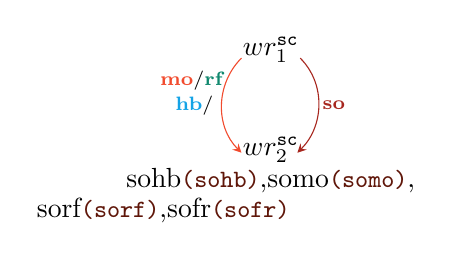
\begin{tikzpicture}[x=1em,y=1em,yscale=-1,xscale=-1]
\tikzstyle{every node}=[font=\normalfont]
\node (wr1) {$ wr^\sc_1 $};
\node (wr2) [below=20pt of wr1] {$ wr^\sc_2 $};
\node (so1) [below=-5pt of wr2] {\hlref{sohb},\hlref{somo},};
\node (so2) [below left=-5pt and -66pt of so1] {\hlref{sorf},\hlref{sofr}};

\draw [->,>=stealth,color=Mahogany,thin] ($ (wr1.south east)+(.3,-5pt) $) to[out=135,in=-135] node[midway,right=-2pt,font=\scriptsize] {\textcolor{black}{\lso}} ($ (wr2.south east)+(0.4,-7pt) $);
\draw [->,>=stealth,color=RedOrange,thin] ($ (wr1.south west)+(-.3,-5pt) $) to[out=45,in=-45] node[left=-2pt,pos=.25,font=\scriptsize] {\textcolor{black}{\lmo/\lrf}} node[left=-0.5pt,pos=.5,font=\scriptsize] {\textcolor{black}{\lhb/\lfr}} ($ (wr2.south west)+(-0.3,-7pt) $);




%\node (nodeB) {$ b: r_1 \assign x  $};
%\node (sigB1) [below left=-3pt and -5pt of nodeB, color=green] {$\sigma_{b11} = $};
%\node (poB1empty) [right=-1pt of sigB1, color=green] {$ $};
%\node (poB1) [draw,fit=(poB1empty), color=orange, thin, inner sep=0pt] {};
%%\node (poB1n1) [right=-3pt of sigB1, color=green] {$ $};
%%\node (poB1) [draw,fit=(poB1n1), color=orange, thin, inner sep=0pt] {};
%\node (B1Val) [right=-3pt of poB1, color=green] {$,0$};
%\node (sigB1State) [fit=(poB1)(B1Val)(sigB1), inner sep=-1pt] {}; 

%\node (sigB2) [right=-3pt of sigB1State, color=green] {$\sigma_{b22} = $};
%\node (poB2N1) [right=6pt of sigB2, circle,fill=black,inner sep=0pt,minimum size=3pt] {};
%\node (poB2a) [left=1pt of poB2N1, inner sep=1pt] {$a$};
%\node (poB2) [draw,fit=(poB2N1)(poB2a), color=orange, thin, inner sep=1pt] {};
%\node (B2Val) [right=-3pt of poB2, color=green] {$,1$};
%\node (sigB2State) [fit=(poB2)(B2Val)(sigB2), inner sep=0pt] {}; 
%
%
%
%%\node (rhoB1) [below =10pt of sigB1State, color=red] {$\rho_{b1}:=0$};
%%\node (rhoB2) [below =10pt of sigB2State, color=red] {$\rho_{b2}:=1$};
%
%
%\node (nodeC) [below =2 of nodeB] {$c: x \assign 2$};
%\node (sigC1) [below left=3pt and -4pt of nodeC, color=green] {$\sigma_{c11} = $};
%\node (poC1N1) [right=6pt of sigC1, circle,fill=black,inner sep=0pt,minimum size=3pt] {};
%\node (poC1c) [left=1pt of poC1N1, inner sep=1pt] {$c$};
%\node (poC1) [draw,fit=(poC1c)(poC1N1), color=orange, thin, inner sep=1pt] {};
%\node (C1Val) [right=-3pt of poC1, color=green] {$,2$};
%\node (sigC1State) [fit=(poC1)(C1Val)(sigC1), inner sep=0pt] {}; 
%
%\node (sigC2) [right=-3pt of sigC1State, color=green] {$\sigma_{c22} = $};
%\node (poC2n1) [above right=0pt and 5pt of sigC2, circle,fill=black,inner sep=0pt,minimum size=3pt] {};
%\node (poC2a) [left=1pt of poC2n1, inner sep=0pt] {$a$};
%\node (poC2n2) [below=9pt of poC2n1, circle,fill=black,inner sep=0pt,minimum size=3pt] {};
%\node (poC2c) [left=1pt of poC2n2, inner sep=0pt] {$c$};
%\draw [color=purple] (poC2n1) -- (poC2n2);
%\node (poC2) [draw,fit=(poC2n1)(poC2a)(poC2n2)(poC2c), color=orange, thin, inner sep=1pt] {};
%\node (C2Val) [right=-3pt of poC2, color=green] {$,2$};
%\node (sigC2State) [fit=(poC2)(C2Val)(sigC2), inner sep=0pt] {}; 
%
%
%
%%\node (rhoC) [below=30pt of nodeC, color=red] {$\rho_{c}=2$};
%
%\node (nodeA) [left =3.5 of nodeB] {$a: x \assign 1$};
%\node (sigA) [below left=-2pt and -25pt of nodeA, color=green] {$\sigma_{a11} = $};
%\node (poAN1) [right=6pt of sigA, circle,fill=black,inner sep=0pt,minimum size=3pt] {};
%\node (poAa) [left=1pt of poAN1, inner sep=1pt] {$a$};
%\node (poA) [draw,fit=(poAN1)(poAa), color=orange, thin, inner sep=1pt] {};
%\node (AVal) [right=-3pt of poA, color=green] {$,1$};
%\node (sigAState) [fit=(poA)(AVal)(sigA), inner sep=-1pt] {}; 
%
%%\node (rhoA) [below=1pt of sigAState, color=red] {$\rho_{a} := 1$};
%
%
%\node (nodeD) [right =5.5 of nodeB] {$ d: r_2 \assign x  $};
%\node (sigD1) [below left=3pt and -5pt of nodeD, color=green] {$\sigma_{d22} = $};
%\node (poD1N1) [right=6pt of sigD1, circle,fill=black,inner sep=0pt,minimum size=3pt] {};
%\node (poD1c) [left=1pt of poD1N1, inner sep=1pt] {$c$};
%\node (poD1) [draw,fit=(poD1c)(poD1N1), color=orange, thin, inner sep=1pt] {};
%\node (D1Val) [right=-3pt of poD1, color=green] {$,2$};
%\node (sigD1State) [fit=(poD1)(D1Val)(sigD1), inner sep=0pt] {}; 
%
%\node (sigD2) [right=-3pt of sigD1State, color=green] {$\sigma_{d33} = $};
%\node (poD2n1) [above right=0pt and 5pt of sigD2, circle,fill=black,inner sep=0pt,minimum size=3pt] {};
%\node (poD2a) [left=1pt of poD2n1, inner sep=0pt] {$a$};
%\node (poD2n2) [below=9pt of poD2n1, circle,fill=black,inner sep=0pt,minimum size=3pt] {};
%\node (poD2c) [left=1pt of poD2n2, inner sep=0pt] {$c$};
%\draw [color=purple] (poD2n1) -- (poD2n2);
%\node (poD2) [draw,fit=(poD2n1)(poD2a)(poD2n2)(poD2c), color=orange, thin, inner sep=1pt] {};
%\node (D2Val) [right=-3pt of poD2, color=green] {$,2$};
%\node (sigD2State) [fit=(poD2)(D2Val)(sigD2), inner sep=0pt] {};  
%
%
%
%\node (nodeE) [below =2 of nodeD] {$e: r_3 \assign x$};
%\node (sigE1) [below left=3pt and -5pt of nodeE, color=green] {$\sigma_{e23} = $};
%\node (poE1N1) [right=6pt of sigE1, circle,fill=black,inner sep=0pt,minimum size=3pt] {};
%\node (poE1c) [left=1pt of poE1N1, inner sep=1pt] {$c$};
%\node (poE1) [draw,fit=(poE1c)(poE1N1), color=orange, thin, inner sep=1pt] {};
%\node (E1Val) [right=-3pt of poE1, color=green] {$,2$};
%\node (sigE1State) [fit=(poE1)(E1Val)(sigE1), inner sep=0pt] {}; 
%
%\node (sigE2) [right=-3pt of sigE1State, color=green] {$\sigma_{e34} = $};
%\node (poE2n1) [above right=0pt and 5pt of sigE2, circle,fill=black,inner sep=0pt,minimum size=3pt] {};
%\node (poE2a) [left=1pt of poE2n1, inner sep=0pt] {$a$};
%\node (poE2n2) [below=9pt of poE2n1, circle,fill=black,inner sep=0pt,minimum size=3pt] {};
%\node (poE2c) [left=1pt of poE2n2, inner sep=0pt] {$c$};
%\draw [color=purple] (poE2n1) -- (poE2n2);
%\node (poE2) [draw,fit=(poE2n1)(poE2a)(poE2n2)(poE2c), color=orange, thin, inner sep=1pt] {};
%\node (E2Val) [right=-3pt of poE2, color=green] {$,2$};
%\node (sigE2State) [fit=(poE2)(E2Val)(sigE2), inner sep=0pt] {}; 
%
%\node (sigE3) [below =9pt of sigE1, color=green] {$\sigma_{e32} = $};
%\node (poE3n1) [above right=0pt and 5pt of sigE3, circle,fill=black,inner sep=0pt,minimum size=3pt] {};
%\node (poE3c) [left=1pt of poE3n1, inner sep=0pt] {$c$};
%\node (poE3n2) [below=9pt of poE3n1, circle,fill=black,inner sep=0pt,minimum size=3pt] {};
%\node (poE3a) [left=1pt of poE3n2, inner sep=0pt] {$a$};
%\draw [color=purple] (poE3n1) -- (poE3n2);
%\node (poE3) [draw,fit=(poE3n1)(poE3a)(poE3n2)(poE3c), color=orange, thin, inner sep=1pt] {};
%\node (E3Val) [right=-3pt of poE3, color=green] {$,1$};
%\node (sigE3State) [fit=(poE3)(E3Val)(sigE3), inner sep=0pt] {};
%
%\node (sigE4) [right =-11pt of sigE3State, color=green] {$\quad \sigma_{e35} = \bot$};
%\node (sigE4State) [fit=(sigE4), inner sep=1pt] {};
%
%
%
%
%%\draw [dashed,->,>=stealth,color=brown,thin] (sigB1State.west) to[out=45,in=-45] (sigC1State.west);
%%\draw [dashed,->,>=stealth,color=brown,thin] (sigB2State.west) to[out=45,in=-45] (sigC2State.west);
%%\draw [dashed,->,>=stealth,color=brown,thin] (sigD1State.west) to[out=45,in=-45] (sigE1State.west);
%%\draw [dashed,->,>=stealth,color=brown,thin] (sigD2State.west) to[out=45,in=-45] (sigE2State.west);
%%\draw [dashed,->,>=stealth,color=brown,thin] (sigD1State.east) to[out=135,in=-135] (sigE3State.east);
%%\draw [dashed,->,>=stealth,color=brown,thin] (sigD2State.east) to[out=135,in=-135] (sigE4State.east);
%%\draw [dashed,->,>=stealth,color=blue,thin] (sigC1State.north east) to[out=-110,in=0] node[midway,left] {rf} (sigD1State.west);
%%\draw [dashed,->,>=stealth,color=blue,thin] (sigC2State.east) to[out=-150,in=0] node[midway,left] {rf} (sigD2State.west);
%
%\draw [dashed,->,>=stealth,color=blue,thin] (sigAState) to[out=165,in=25] node[midway,above] {rf} (sigB2State.south);
%\draw [dashed,->,>=stealth,color=blue,thin] (sigC1State.north east) -- node[midway,above] {rf} (sigD1State.south west);
%\draw [dashed,->,>=stealth,color=blue,thin] (sigC2State.north east) -- node[midway,above] {rf} (sigD2State.south west);
%\draw [dashed,->,>=stealth,color=blue,thin] (sigAState) to[out=105,in=15] node[midway,above] { rf} (sigE3State.west);
%\draw [dashed,->,>=stealth,color=blue,thin] (sigAState) to[out=100,in=20] node[midway,above] {rf} (sigE4State.south);

%\draw [dashed,->,>=stealth,color=blue,thin] (rhoA) -- node[midway,above] {rf} (rhoB2);
%\vspace{-10pt}
\end{tikzpicture}
} &
		\resizebox{0.24\textwidth}{!}{\tikzset{every picture/.style={line width=0.75pt}} %set default line width to 0.75pt        
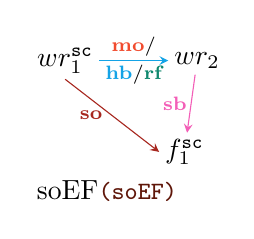
\begin{tikzpicture}[x=1em,y=1em,yscale=-1,xscale=-1]
\tikzstyle{every node}=[font=\normalfont]
\node (wr1) [inner sep=2pt] {$ wr^\sc_1 $};
\node (wr2) [right=25pt of wr1,inner sep=2pt] {$ wr_2 $};
\node (f1) [below left=21pt and -15pt of wr2,inner sep=2pt] {$ f^\sc_1 $};
\node (soef) [below left=0pt and -10pt of f1] {\hlref{soEF}};

`\draw [->,>=stealth,color=Mahogany,thin] (wr1.south) -- node[midway,left=0pt,font=\scriptsize,color=black] { $\lso$ } (f1.west);
\draw [->,>=stealth,color=Cerulean,thin] (wr1) -- node[midway,above=-2pt,font=\scriptsize,color=black] { $ \lmo/ $ } node[midway,below=-2pt,font=\scriptsize,color=black] { $ \lhb/\lrf $ } (wr2);
\draw [->,>=stealth,color=CarnationPink,thin] (wr2) -- node[midway,left=-2pt,font=\scriptsize,color=black] { $\lsb$ } (f1);

\end{tikzpicture}
} &
		\resizebox{0.24\textwidth}{!}{\tikzset{every picture/.style={line width=0.75pt}} %set default line width to 0.75pt        
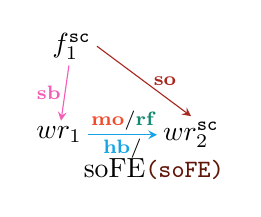
\begin{tikzpicture}[x=1em,y=1em,yscale=-1,xscale=-1]
\tikzstyle{every node}=[font=\normalfont]
\node [inner sep=2pt] (f1) {$ f^\sc_1 $};
\node (wr1) [below left=20pt and -15pt of f1,inner sep=2pt] {$ wr_1 $};
\node (wr2) [right=25pt of wr1,inner sep=2pt] {$ wr^\sc_2 $};
\node (sofe) [below right=0pt and -5pt of wr1] {\hlref{soFE}};

`\draw [->,>=stealth,color=Mahogany] (f1.east) -- node[midway,right=0pt,font=\scriptsize,color=black] { $\lso$ } (wr2.north);
\draw [->,>=stealth,color=Cerulean] (wr1) -- node[midway,above=-2pt,font=\scriptsize,color=black] { $ \lmo/\lrf $ } node[midway,below=-2pt,font=\scriptsize,color=black] { $ \lhb/\lfr $ } (wr2);
\draw [->,>=stealth,color=CarnationPink] (f1) -- node[midway,left=-2pt,font=\scriptsize,color=black] { $\lsb$ } (wr1);

\end{tikzpicture}
} &
		\resizebox{0.24\textwidth}{!}{\tikzset{every picture/.style={line width=0.75pt}} %set default line width to 0.75pt        
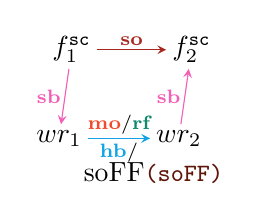
\begin{tikzpicture}[x=1em,y=1em,yscale=-1,xscale=-1]
\tikzstyle{every node}=[font=\normalfont]
\node (f1) [inner sep=2pt] {$ f^\sc_1 $};
\node (f2) [right=25pt of f1,inner sep=2pt] {$ f^\sc_2 $};
\node (wr1) [below left=20pt and -15pt of f1,inner sep=2pt] {$ wr_1 $};
\node (wr2) [below left=20pt and -15pt of f2,inner sep=2pt] {$ wr_2 $};
\node (soff) [below right=0pt and -5pt of wr1] {\hlref{soFF}};

`\draw [->,>=stealth,color=Mahogany] (f1) -- node[midway,above=-2pt,font=\scriptsize,color=black] { $\lso$ } (f2);
\draw [->,>=stealth,color=Cerulean] (wr1) -- node[midway,above=-2pt,font=\scriptsize,color=black]{\lmo/\lrf} node[midway,below=-2pt,font=\scriptsize,color=black]{ $ \lhb/\lfr $ } (wr2);
\draw [->,>=stealth,color=CarnationPink] (f1) -- node[midway,left=-2pt,font=\scriptsize,color=black] { $\lsb$ } (wr1);
\draw [->,>=stealth,color=CarnationPink] (wr2) -- node[midway,left=-2pt,font=\scriptsize,color=black] { $\lsb$ } (f2);

%\draw [->,>=stealth,color=orange] ($ (ew1.south east)+(.5,-5pt) $) to[out=135,in=-135] node[midway,right=-2pt,font=\scriptsize] {mo} ($ (ew2.south east)+(0.4,-5pt) $);
%\draw [->,>=stealth,color=red] ($ (ew1.south west)+(-.3,-5pt) $) to[out=45,in=-45] node[midway,left=-2pt,font=\scriptsize] {c::hb} ($ (ew2.south west)+(-0.3,-5pt) $);


\end{tikzpicture}
} \\
		\hline
%		\hline

%		\resizebox{0.24\textwidth}{!}{\tikzset{every picture/.style={line width=0.75pt}} %set default line width to 0.75pt        
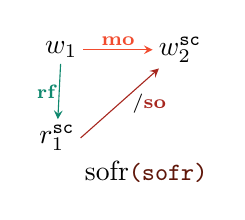
\begin{tikzpicture}[x=1em,y=1em,yscale=-1,xscale=-1]
\tikzstyle{every node}=[font=\normalfont]
\node (w1) [inner sep=2pt] {$ w_1 $};
\node (w2) [right=25pt of w1,inner sep=2pt] {$ w^\sc_2 $};
\node (r1) [below left=20pt and -15pt of w1,inner sep=2pt] {$ r^\sc_1 $};
\node (sofr) [below right=-2pt and -2pt of r1] {\hlref{sofr}};

%\draw [->,>=stealth,color=Mahogany,thin] (er1)+(-7pt, 0) -- node[midway,above=-2pt,font=\scriptsize,color=black] { $\lchb$ } (ew1)+(7pt, 0);
\draw [->,>=stealth,color=RedOrange,thin] (w1) -- node[midway,above=-2pt,font=\scriptsize,color=black] { $\lmo$ } (w2);
\draw [->,>=stealth,color=Mahogany,thin] (r1.east) -- 
node[midway,right=1pt,font=\scriptsize,color=black] { $\lfr/\lso$ } (w2);
\draw [->,>=stealth,color=PineGreen,thin] (w1) -- node[midway,left=-2pt,font=\scriptsize,color=black] { $\lrf$ } (r1);`

\end{tikzpicture}
} &
%		\resizebox{0.24\textwidth}{!}{\tikzset{every picture/.style={line width=0.75pt}} %set default line width to 0.75pt        
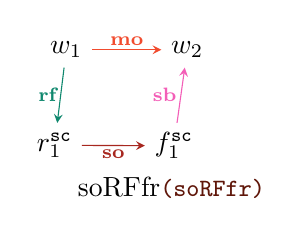
\begin{tikzpicture}[x=1em,y=1em,yscale=-1,xscale=-1]
\tikzstyle{every node}=[font=\normalfont]
\node (w1) {$ w_1 $};
\node (w2) [right=25pt of w1] {$ w_2 $};
\node (r1) [below left=20pt and -15pt of w1] {$ r^\sc_1 $};
\node (f1) [below left=20pt and -15pt of w2] {$ f^\sc_1 $};
\node (sorffr) [below right=0pt and -5pt of r1] {\hlref{soRFfr}};

`\draw [->,>=stealth,color=RedOrange,thin] (w1) -- node[midway,above=-2pt,font=\scriptsize,color=black] { $\lmo$ } (w2);
\draw [->,>=stealth,color=PineGreen,thin] (w1) -- node[midway,left=-2pt,font=\scriptsize,color=black] { $ \lrf $ } (r1);
\draw [->,>=stealth,color=CarnationPink,thin] (f1) -- node[midway,left=-2pt,font=\scriptsize,color=black] { $\lsb$ } (w2);
\draw [->,>=stealth,color=Mahogany,thin] (r1) -- node[midway,below=-2pt,font=\scriptsize,color=black] { $\lso$ } (f1);

\end{tikzpicture}
} &
%		\resizebox{0.24\textwidth}{!}{\tikzset{every picture/.style={line width=0.75pt}} %set default line width to 0.75pt        
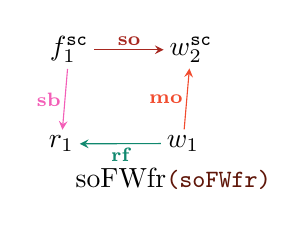
\begin{tikzpicture}[x=1em,y=1em,yscale=-1,xscale=-1]
\tikzstyle{every node}=[font=\normalfont]
\node (f1) [inner sep=2pt] {$ f^\sc_1 $};
\node (w2) [right=25pt of f1,inner sep=2pt] {$ w^\sc_2 $};
\node (r1) [below left=22pt and -13pt of f1,inner sep=2pt] {$ r_1 $};
\node (w1) [below left=22pt and -15pt of w2,inner sep=2pt] {$ w_1 $};
\node (sofwfr) [below right=0pt and -5pt of r1] {\hlref{soFWfr}};

`\draw [->,>=stealth,color=Mahogany,thin] (f1) -- node[midway,above=-2pt,font=\scriptsize,color=black] { $\lso$ } (w2);
\draw [->,>=stealth,color=PineGreen,thin] (w1) -- node[midway,below=-2pt,font=\scriptsize,color=black] { $ \lrf $ } (r1);
\draw [->,>=stealth,color=CarnationPink,thin] (f1) -- node[midway,left=-2pt,font=\scriptsize,color=black] { $\lsb$ } (r1);
\draw [->,>=stealth,color=RedOrange,thin] (w1) -- node[midway,left=-2pt,font=\scriptsize,color=black] { $\lmo$ } (w2);

\end{tikzpicture}
} &
%		\resizebox{0.24\textwidth}{!}{\tikzset{every picture/.style={line width=0.75pt}} %set default line width to 0.75pt        
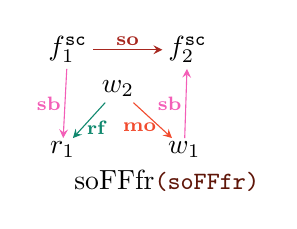
\begin{tikzpicture}[x=1em,y=1em,yscale=-1,xscale=-1]
\tikzstyle{every node}=[font=\normalfont]
\node (f1) [inner sep=2pt] {$ f^\sc_1 $};
\node (f2) [right=25pt of f1,inner sep=2pt] {$ f^\sc_2 $};
\node (r1) [below left=25pt and -13pt of f1, inner sep=1pt] {$ r_1 $};
\node (w1) [below left=25pt and -15pt of f2, inner sep=1pt] {$ w_1 $};
\node (w2) [below right=2pt and 1pt of f1,inner sep=2pt] {$ w_2 $};
\node (sofffr) [below right=0pt and -5pt of r1] {\hlref{soFFfr}};

`\draw [->,>=stealth,color=RedOrange,thin] (w2) -- node[pos=0.7,left=-2pt,font=\scriptsize,color=black] { $\lmo$ } (w1);
\draw [->,>=stealth,color=PineGreen,thin] (w2) -- node[pos=0.7,right=-2pt,font=\scriptsize,color=black] { $ \lrf $ } (r1);
\draw [->,>=stealth,color=CarnationPink,thin] (f1) -- node[midway,left=-2pt,font=\scriptsize,color=black] { $\lsb$ } (r1);
\draw [->,>=stealth,color=CarnationPink,thin] (w1) -- node[midway,left=-2pt,font=\scriptsize,color=black] { $\lsb$ } (f2);
\draw [->,>=stealth,color=Mahogany,thin] (f1) -- node[midway,above=-2pt,font=\scriptsize,color=black] { $\lso$ } (f2);

\end{tikzpicture}
} \\
%		\hline
%		
%		\multicolumn{1}{c||}{} & 
%		\resizebox{0.24\textwidth}{!}{\tikzset{every picture/.style={line width=0.75pt}} %set default line width to 0.75pt        
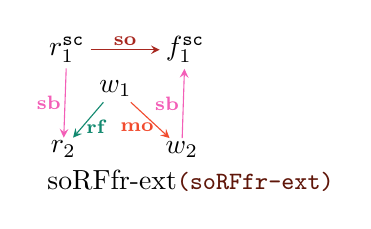
\begin{tikzpicture}[x=1em,y=1em,yscale=-1,xscale=-1]
\tikzstyle{every node}=[font=\normalfont]
\node (r1) [inner sep=2pt] {$ r^\sc_1 $};
\node (f1) [right=25pt of r1,inner sep=2pt] {$ f^\sc_1 $};
\node (r2) [below left=25pt and -13pt of r1, inner sep=1pt] {$ r_2 $};
\node (w2) [below left=25pt and -15pt of f1, inner sep=1pt] {$ w_2 $};
\node (w1) [below right=2pt and 1pt of r1,inner sep=2pt] {$ w_1 $};
\node (sorffrext) [below right=0pt and -15pt of r2] {\hlref{soRFfr-ext}};

`\draw [->,>=stealth,color=RedOrange,thin] (w1) -- node[pos=0.7,left=-2pt,font=\scriptsize,color=black] { $\lmo$ } (w2);
\draw [->,>=stealth,color=PineGreen,thin] (w1) -- node[pos=0.7,right=-2pt,font=\scriptsize,color=black] { $ \lrf $ } (r2);
\draw [->,>=stealth,color=CarnationPink,thin] (r1) -- node[midway,left=-2pt,font=\scriptsize,color=black] { $\lsb$ } (r2);
\draw [->,>=stealth,color=CarnationPink,thin] (w2) -- node[midway,left=-2pt,font=\scriptsize,color=black] { $\lsb$ } (f1);
\draw [->,>=stealth,color=Mahogany,thin] (r1) -- node[midway,above=-2pt,font=\scriptsize,color=black] { $\lso$ } (f1);

\end{tikzpicture}
} &
%		\resizebox{0.24\textwidth}{!}{\tikzset{every picture/.style={line width=0.75pt}} %set default line width to 0.75pt        
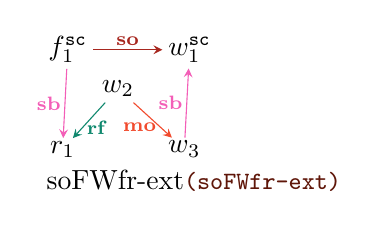
\begin{tikzpicture}[x=1em,y=1em,yscale=-1,xscale=-1]
\tikzstyle{every node}=[font=\normalfont]
\node (f1) [inner sep=2pt] {$ f^\sc_1 $};
\node (wx) [right=25pt of f1,inner sep=2pt] {$ w^\sc_1 $};
\node (r1) [below left=25pt and -13pt of f1, inner sep=1pt] {$ r_1 $};
\node (w2) [below left=25pt and -15pt of wx, inner sep=1pt] {$ w_3 $};
\node (w1) [below right=2pt and 1pt of f1,inner sep=2pt] {$ w_2 $};
\node (sofwfrext) [below right=0pt and -15pt of r1] {\hlref{soFWfr-ext}};

`\draw [->,>=stealth,color=RedOrange,thin] (w1) -- node[pos=0.7,left=-2pt,font=\scriptsize,color=black] { $\lmo$ } (w2);
\draw [->,>=stealth,color=PineGreen,thin] (w1) -- node[pos=0.7,right=-2pt,font=\scriptsize,color=black] { $ \lrf $ } (r1);
\draw [->,>=stealth,color=CarnationPink,thin] (f1) -- node[midway,left=-2pt,font=\scriptsize,color=black] { $\lsb$ } (r1);
\draw [->,>=stealth,color=CarnationPink,thin] (w2) -- node[midway,left=-2pt,font=\scriptsize,color=black] { $\lsb$ } (wx);
\draw [->,>=stealth,color=Mahogany,thin] (f1) -- node[midway,above=-2pt,font=\scriptsize,color=black] { $\lso$ } (wx);

\end{tikzpicture}
} & 
%		\multicolumn{1}{|c}{}\\
%		\cline{2-3}
	\end{tabular}
	\caption{\lso-rules}
	\label{fig:so rules}
\end{figure}

\begin{figure}[t]
	\begin{tabular}{|c||c|c|c|}
		\multicolumn{1}{c}{base rule} & 
		\multicolumn{3}{c}{extended fence rules} \\\hline
		
		\resizebox{0.24\textwidth}{!}{\tikzset{every picture/.style={line width=0.75pt}} %set default line width to 0.75pt        
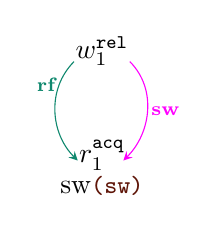
\begin{tikzpicture}[x=1em,y=1em,yscale=-1,xscale=-1]
\tikzstyle{every node}=[font=\normalfont]
\node (w1) {$ w^\rel_1 $};
\node (r1) [below=20pt of w1] {$ r^\acq_1 $};
\node (sw) [below=-5pt of r1] {\hlref{sw}};

\draw [->,>=stealth,color=Magenta] ($ (w1.south east)+(.3,-5pt) $) to[out=135,in=-135] node[midway,right=-2pt,font=\scriptsize] {\textcolor{black}{\lsw}} ($ (r1.south east)+(0.4,-7pt) $);
\draw [->,>=stealth,color=PineGreen] ($ (w1.south west)+(-.3,-5pt) $) to[out=45,in=-45] node[left=-2pt,pos=.25,font=\scriptsize] {\textcolor{black}{\lrf}}($ (r1.south west)+(-0.3,-7pt) $);

\end{tikzpicture}
} &
		\resizebox{0.24\textwidth}{!}{\tikzset{every picture/.style={line width=0.75pt}} %set default line width to 0.75pt        
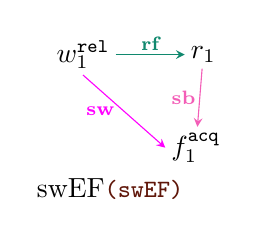
\begin{tikzpicture}[x=1em,y=1em,yscale=-1,xscale=-1]
\tikzstyle{every node}=[font=\normalfont]
\node (w1) [inner sep=2pt] {$ w^\rel_1 $};
\node (r1) [right=25pt of w1,inner sep=2pt] {$ r_1 $};
\node (f1) [below left=21pt and -15pt of r1,inner sep=2pt] {$ f^\acq_1 $};
\node (swef) [below left=0pt and -10pt of f1] {\hlref{swEF}};

`\draw [->,>=stealth,color=Magenta,thin] (w1.south) -- node[midway,left=0pt,font=\scriptsize,color=black] { $\lsw$ } (f1.west);
\draw [->,>=stealth,color=PineGreen,thin] (w1) -- node[midway,above=-2pt,font=\scriptsize,color=black] { $ \lrf $ }  (r1);
\draw [->,>=stealth,color=CarnationPink,thin] (r1) -- node[midway,left=-2pt,font=\scriptsize,color=black] { $\lsb$ } (f1);

\end{tikzpicture}
} &
		\resizebox{0.24\textwidth}{!}{\tikzset{every picture/.style={line width=0.75pt}} %set default line width to 0.75pt        
\begin{tikzpicture}[x=1em,y=1em,yscale=-1,xscale=-1]
\tikzstyle{every node}=[font=\normalfont]
\node [inner sep=2pt] (f1) {$ f^\rel_1 $};
\node (w1) [below left=21pt and -15pt of f1,inner sep=2pt] {$ w_1 $};
\node (r1) [right=25pt of w1,inner sep=2pt] {$ r^\acq_1 $};
\node (swfe) [below right=0pt and -15pt of wr1] {\hlref{sw-dobFE}};

`\draw [->,>=stealth,color=Magenta,thin] (f1.east) -- node[midway,right=0pt,font=\scriptsize,color=black] { $\lsw$ } (r1.north);
\draw [->,>=stealth,color=PineGreen,thin] (w1) -- node[midway,above=-2pt,font=\scriptsize,color=black] { $ \lrf $ } (r1);
\draw [->,>=stealth,color=CarnationPink,thin] (f1) -- node[midway,left=-2pt,font=\scriptsize,color=black] { $\lsb$ } (w1);

\end{tikzpicture}
} &
		\resizebox{0.24\textwidth}{!}{\tikzset{every picture/.style={line width=0.75pt}} %set default line width to 0.75pt        
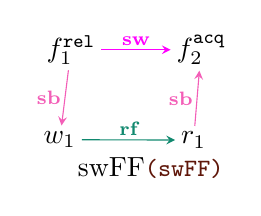
\begin{tikzpicture}[x=1em,y=1em,yscale=-1,xscale=-1]
\tikzstyle{every node}=[font=\normalfont]
\node (f1) [inner sep=2pt] {$ f^\rel_1 $};
\node (f2) [right=25pt of f1,inner sep=2pt] {$ f^\acq_2 $};
\node (w1) [below left=20pt and -15pt of f1,inner sep=2pt] {$ w_1 $};
\node (r1) [below left=20pt and -15pt of f2,inner sep=2pt] {$ r_1 $};
\node (swff) [below right=-2pt and -5pt of w1] {\hlref{swFF}};

`\draw [->,>=stealth,color=Magenta] (f1) -- node[midway,above=-2pt,font=\scriptsize,color=black] { $\lsw$ } (f2);
\draw [->,>=stealth,color=PineGreen] (w1) -- node[midway,above=-2pt,font=\scriptsize,color=black]{\lrf} (r1);
\draw [->,>=stealth,color=CarnationPink] (f1) -- node[midway,left=-2pt,font=\scriptsize,color=black] { $\lsb$ } (w1);
\draw [->,>=stealth,color=CarnationPink] (r1) -- node[midway,left=-2pt,font=\scriptsize,color=black] { $\lsb$ } (f2);

%\draw [->,>=stealth,color=orange] ($ (ew1.south east)+(.5,-5pt) $) to[out=135,in=-135] node[midway,right=-2pt,font=\scriptsize] {mo} ($ (ew2.south east)+(0.4,-5pt) $);
%\draw [->,>=stealth,color=red] ($ (ew1.south west)+(-.3,-5pt) $) to[out=45,in=-45] node[midway,left=-2pt,font=\scriptsize] {c::hb} ($ (ew2.south west)+(-0.3,-5pt) $);


\end{tikzpicture}
} \\
		
		\resizebox{0.24\textwidth}{!}{\tikzset{every picture/.style={line width=0.75pt}} %set default line width to 0.75pt        
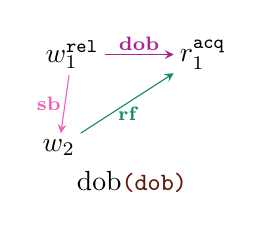
\begin{tikzpicture}[x=1em,y=1em,yscale=-1,xscale=-1]
\tikzstyle{every node}=[font=\normalfont]
\node (w1) [inner sep=2pt] {$ w^\rel_1 $};
\node (r1) [right=25pt of w1,inner sep=2pt] {$ r^\acq_1 $};
\node (w2) [below left=21pt and -15pt of w1,inner sep=2pt] {$ w_2 $};
\node (dob) [below right=0pt and -5pt of w2] {\hlref{dob}};

`\draw [->,>=stealth,color=Mulberry] (w1.east) -- node[midway,above=-2pt,font=\scriptsize,color=black] { $\ldob$ } (r1.west);
\draw [->,>=stealth,color=PineGreen] (w2) -- node[midway,below=-2pt,font=\scriptsize,color=black] { $ \lrf $ }  (r1);
\draw [->,>=stealth,color=CarnationPink] (w1) -- node[midway,left=-2pt,font=\scriptsize,color=black] { $\lsb$ } (w2);

\end{tikzpicture}
} &
		\resizebox{0.24\textwidth}{!}{\tikzset{every picture/.style={line width=0.75pt}} %set default line width to 0.75pt        
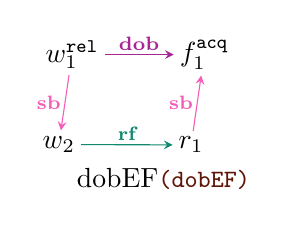
\begin{tikzpicture}[x=1em,y=1em,yscale=-1,xscale=-1]
\tikzstyle{every node}=[font=\normalfont]
\node (w1) [inner sep=2pt] {$ w^\rel_1 $};
\node (f1) [right=25pt of w1,inner sep=2pt] {$ f^\acq_1 $};
\node (w2) [below left=20pt and -15pt of w1,inner sep=2pt] {$ w_2 $};
\node (r1) [below left=20pt and -13pt of f1,inner sep=2pt] {$ r_1 $};
\node (dobEF) [below right=0pt and -5pt of w2] {\hlref{dobEF}};

`\draw [->,>=stealth,color=PineGreen,thin] (w2) -- node[midway,above=-2pt,font=\scriptsize,color=black] { $\lrf$ } (r1);
\draw [->,>=stealth,color=CarnationPink,thin] (w1) -- node[midway,left=-2pt,font=\scriptsize,color=black] { $ \lsb $ } (w2);
\draw [->,>=stealth,color=CarnationPink,thin] (r1) -- node[midway,left=-2pt,font=\scriptsize,color=black] { $\lsb$ } (f1);
\draw [->,>=stealth,color=Mulberry,thin] (w1) -- node[midway,above=-2pt,font=\scriptsize,color=black] { $\ldob$ } (f1);

\end{tikzpicture}
} &&\\
		\hline
		
	\end{tabular}
	\caption{\lsw-rules}
	\label{fig:sw rules}
\end{figure}

\begin{longtable}{|p{0.11\textwidth} p{0.88\textwidth}|}
	\hline
	\multicolumn{2}{|l|}{\bf $\setHB$, $\setMO$, $\setRF$ base rules:}\\
	
	\hl{sohb}, \hl{somo},  & 
	$\forall wr^{\sc}_1, wr^{\sc}_2 \in \ordevents{\sc}_\tau$ if 
	$\hb{\tau}{wr^{\sc}_1}{wr^{\sc}_2}$ $\v$ $\mo{\tau}{wr^{\sc}_1}{wr^{\sc}_2}$
	$\v$ $\rf{\tau}{wr^{\sc}_1}{wr^{\sc}_2}$ then 
	$\so{\tau}{wr^{\sc}_1}{wr^{\sc}_2}$ \\
	\hl{sorf}: & ($\setHB$ order implies $\setSO$) \\
	
%	\hl{somo}: & $\forall w^{\sc}_1, w^{\sc}_2 \in \ordwrites{\sc}_\tau$ if 
%	$\mo{\tau}{w^{\sc}_1}{w^{\sc}_2}$
%	then $\so{\tau}{w^{\sc}_1}{w^{\sc}_2}$ \\
%	& ($\setMO$ order implies $\setSO$) \\
%	
%	\hl{sorf}: & $\forall w^{\sc}_1 \in \ordwrites{sc}_\tau$, $r^{\sc}_1 \in 
%	\ordreads{\sc}_\tau$ if $\rf{\tau}{w^{\sc}_1}{r^{\sc}_1}$ then 
%	$\so{\tau}{w^{\sc}_1}{r^{\sc}_1}$ \\
%	& ($\setRF$ order implies $\setSO$) \\
	& \\
	
	\multicolumn{2}{|l|}{\bf $\setHB$, $\setMO$, $\setRF$ rules extended
		for fences:} \\
	
	\hl{soEF}: & $\forall wr^\sc_1 \in \ordevents{\sc}_\tau$, $f^\sc_1 \in
	\ordfences{\sc}_\tau$ if $\exists wr_2 \in \events_\tau$ \st 
	($\mo{\tau}{wr^\sc_1}{wr_2}$ $\v$ $\hb{\tau}{wr^\sc_1}{wr_2}$
	$\v$ $\rf{\tau}{wr^\sc_1}{wr_2}$) $\^$ $\seqb{\tau}{wr_2}{f^\sc_1}$ 
	then $\so{\tau}{wr^\sc_1}{f^\sc_1}$ \\
	& ($\setHB$ between \sc event-fence implies $\setSO$) \\
	
	\hl{soFE}: & $\forall f^\sc_1 \in \ordfences{\sc}_\tau$, $wr^\sc_2 \in
	\ordevents{\sc}_\tau$ if $\exists wr_1 \in \events_\tau$ \st 
	($\mo{\tau}{wr_1}{wr^\sc_2}$ $\v$ $\hb{\tau}{wr_1}{wr^\sc_2}$
	$\v$ $\rf{\tau}{wr_1}{wr^\sc_2}$) $\^$ $\seqb{\tau}{f^\sc_1}{wr_1}$ 
	then $\so{\tau}{f^\sc_1}{wr^\sc_2}$ \\
	& ($\setHB$ between fence-\sc event implies $\setSO$) \\
	
	\hl{soFF}: & $\forall f^{\sc}_1, f^{\sc}_2 \in \ordfences{\sc}_\tau$, 
	if $\exists wr_1, wr_2 \in \events_\tau$ \st 
	($\mo{\tau}{wr_1}{wr_2}$ $\v$ $\hb{\tau}{wr_1}{wr_2}$
	$\v$ $\rf{\tau}{wr_1}{wr_2}$) $\^$
	($\seqb{\tau}{f^{\sc}_1}{wr_1}$, $\seqb{\tau}{wr_2}{f^{\sc}_2}$) 
	then $\so{\tau}{f^{\sc}_1}{f^{\sc}_2}$ \\
	& ($\setHB$ between \sc fence-fences implies $\setSO$) \\
	\hline
\end{longtable}
	
\begin{longtable}{|p{0.13\textwidth} p{0.86\textwidth}|}
	\hline
	\multicolumn{2}{|l|}{\bf $\setFR$ base rule:}\\
	
	\hl{sofr}: & $\forall r^\sc_1 \in \ordreads{\sc}_\tau$, $w^\sc_1 \in
	\ordwrites{\sc}_\tau$ if $\fr{\tau}{r^\sc_1}{w^sc_1}$ then 
	$\so{\tau}{r^{\sc}_1}{w^{\sc}_1}$ \\
	& ($\setFR$ order implies $\setSO$) \\
	
	& \\
	
	\multicolumn{2}{|l|}{\bf $\setFR$ rules extended for fences:}\\
	
	\hl{soRFfr}: & $\forall f^\sc_1 \in \ordfences{\sc}_\tau$, $r^\sc_1 \in
	\ordreads{\sc}_\tau$ if $\exists w_1, w_2 \in \writes_\tau$ \st
	$\seqb{\tau}{w_2}{f^\sc_1}$, $\mo{\tau}{w_1}{w_2}$ and
	$\rf{\tau}{w_1}{r^\sc_1}$ then $\so{\tau}{r^\sc_1}{f^\sc_1}$ \\
	& ($\setFR$ though \sc read-fence synchronization implies $\setSO$) \\
	
	\hl{soRFfr-ext}: & \tab $\forall r^\sc_1 \in \ordreads{\sc}_\tau$, $f^\sc_1 
	\in \ordfences{\sc}_\tau$ if $\exists w_1,w_2 \in \writes_\tau$, $r_2 \in
	\reads_\tau$ \st $\seqb{\tau}{r^\sc_1}{r_2}$, $\seqb{\tau}{w_2}{f^\sc_1}$,
	$\mo{\tau}{w_1}{w_2}$ and $\rf{\tau}{w_1}{r_2}$ then 
	$\so{\tau}{r^\sc_1}{f^\sc_1}$ \\
	& ($\setFR$ though \sc read-fence synchronization via $\setSB$ implies 
	$\setSO$) \\
	
	\hl{soFWfr}: & $\forall f^{\sc}_1 \in \ordfences{\sc}_\tau$, $w^{\sc}_1 \in 
	\ordwrites{\sc}_\tau$ if $\exists w_2 \in \writes_\tau$, $r_1 \in 
	\reads_\tau$ \st $\seqb{\tau}{f^{\sc}_1}{r_1}$, $\mo{\tau}{w_2}{w^{\sc}_1}$ 
	and $\rf{\tau}{w_2}{r_1}$ then $\so{\tau}{f^{\sc}_1}{w^{\sc}_1}$ \\
	& ($\setFR$ though \sc write-fence synchronization implies $\setSO$) \\
	
	\hl{soFWfr-ext}: & \tab $\forall f^{\sc}_1 \in \ordfences{\sc}_\tau$, 
	$w^{\sc}_1 \in \ordwrites{\sc}_\tau$ if $\exists w_2, w_3 \in \writes_\tau$, 
	$r_1 \in \reads_\tau$ \st $\seqb{\tau}{f^{\sc}_1}{r_1}$, 
	$\seqb{\tau}{w_3}{w^\sc_1}$, $\mo{\tau}{w_2}{w_3}$ and $\rf{\tau}{w_2}{r_1}$ 
	then $\so{\tau}{f^\sc_1}{w^\sc_1}$ \\
	& ($\setFR$ though \sc write-fence synchronization via $\setSB$ implies 
	$\setSO$) \\
	
	\hl{soFFfr}: & $\forall f^\sc_1, f^\sc_2 \in \ordfences{\sc}_\tau$
	if $\exists$ $w_1, w_2 \in \ordwrites{\sc}_\tau$, $r_1 \in
	\ordreads{\sc}_\tau$ \st $\seqb{\tau}{f^\sc_1}{r_1}$, 
	$\seqb{\tau}{w_1}{f^\sc_2}$, $\mo{\tau}{w_2}{w_1}$ and
	$\rf{\tau}{w_2}{r_1}$ then $\so{\tau}{f^\sc_1}{f^\sc_2}$ \\
	& ($\setFR$ though \sc fence-fence synchronization implies $\setSO$) \\
	\hline
\end{longtable}


%\begin{itemize}[label=soFFnrf,align=left,leftmargin=*]
%	\item [\hl{sohb}:] $\forall wr^{\sc}_1, wr^{\sc}_2 \in \ordevents{\sc}_\tau$ if 
%			$\hb{\tau}{wr^{\sc}_1}{wr^{\sc}_2}$ then 
%			$\so{\tau}{wr^{\sc}_1}{wr^{\sc}_2}$ \newline
%			($\setHB$ order implies $\setSO$)
%	
%	\item [\hl{somo}:] $\forall w^{\sc}_1, w^{\sc}_2 \in \ordwrites{\sc}_\tau$ if 
%			$\mo{\tau}{w^{\sc}_1}{w^{\sc}_2}$
%			then $\so{\tau}{w^{\sc}_1}{w^{\sc}_2}$ \newline
%			($\setMO$ order implies $\setSO$)
%			
%	\item [\hl{sorf}:] $\forall w^{\sc}_1 \in \ordwrites{sc}_\tau$, $r^{\sc}_1 \in 
%			\ordreads{\sc}_\tau$ if $\rf{\tau}{w^{\sc}_1}{r^{\sc}_1}$ then 
%			$\so{\tau}{w^{\sc}_1}{r^{\sc}_1}$ \newline
%			($\setRF$ order implies $\setSO$)
%			
%	\item [\hl{soEF}:] $\forall wr^\sc_1 \in \ordevents{\sc}_\tau$, $f^\sc_1 \in
%			\ordfences{\sc}_\tau$ if $\exists wr_2 \in \events_\tau$ \st 
%			($\mo{\tau}{wr^\sc_1}{wr_2}$ $\v$ $\hb{\tau}{wr^\sc_1}{wr_2}$
%			$\v$ $\rf{\tau}{wr^\sc_1}{wr_2}$) $\^$ $\seqb{\tau}{wr_2}{f^\sc_1}$ 
%			then $\so{\tau}{wr^\sc_1}{f^\sc_1}$\newline
%			($\setHB$ between \sc event-fence implies $\setSO$)
%			
%	\item [\hl{soFE}:] $\forall f^\sc_1 \in \ordfences{\sc}_\tau$, $wr^\sc_2 \in
%			\ordevents{\sc}_\tau$ if $\exists wr_1 \in \events_\tau$ \st 
%			($\mo{\tau}{wr_1}{wr^\sc_2}$ $\v$ $\hb{\tau}{wr_1}{wr^\sc_2}$
%			$\v$ $\rf{\tau}{wr_1}{wr^\sc_2}$) $\^$ $\seqb{\tau}{f^\sc_1}{wr_1}$ 
%			then $\so{\tau}{f^\sc_1}{wr^\sc_2}$\newline
%			($\setHB$ between fence-\sc event implies $\setSO$)
%			
%	\item [\hl{soFF}:]  $\forall f^{\sc}_1, f^{\sc}_2 \in \ordfences{\sc}_\tau$, 
%			if $\exists wr_1, wr_2 \in \events_\tau$ \st 
%			($\mo{\tau}{wr_1}{wr_2}$ $\v$ $\hb{\tau}{wr_1}{wr_2}$
%			$\v$ $\rf{\tau}{wr_1}{wr_2}$) $\^$
%			($\seqb{\tau}{f^{\sc}_1}{wr_1}$, $\seqb{\tau}{wr_2}{f^{\sc}_2}$) 
%			then $\so{\tau}{f^{\sc}_1}{f^{\sc}_2}$ \newline
%			($\setHB$ between \sc fence-fences implies $\setSO$)
%			
%	\item [\hl{sofr}:] $\forall r^\sc_1 \in \ordreads{\sc}_\tau$, $w^\sc_1 \in
%			\ordwrites{\sc}_\tau$ if $\fr{\tau}{r^\sc_1}{w^sc_1}$ then 
%			$\so{\tau}{r^{\sc}_1}{w^{\sc}_1}$ 
%			\newline
%			($\setFR$ order implies $\setSO$)
%			
%	\item [\hl{soFWfr}:] $\forall f^{\sc}_1 \in \ordfences{\sc}_\tau$, $w^{\sc}_1 \in 
%			\ordwrites{\sc}_\tau$ if $\exists w_2 \in \writes_\tau$, $r_1 \in 
%			\reads_\tau$ \st $\seqb{\tau}{f^{\sc}_1}{r_1}$, $\mo{\tau}{w_2}{w^{\sc}_1}$ 
%			and $\rf{\tau}{w_2}{r_1}$ then $\so{\tau}{f^{\sc}_1}{w^{\sc}_1}$ \newline
%			($\setFR$ though \sc write-fence synchronization implies $\setSO$)
%			
%	\item [\hl{soRFfr}:] $\forall f^\sc_1 \in \ordfences{\sc}_\tau$, $r^\sc_1 \in
%			\ordreads{\sc}_\tau$ if $\exists w_1, w_2 \in \writes_\tau$ \st
%			$\seqb{\tau}{w_2}{f^\sc_1}$, $\mo{\tau}{w_1}{w_2}$ and
%			$\rf{\tau}{w_1}{r^\sc_1}$ then $\so{\tau}{r^\sc_1}{f^\sc_1}$\newline
%			($\setFR$ though \sc read-fence synchronization implies $\setSO$)
%			
%	\item [\hl{soFFfr}:] $\forall f^\sc_1, f^\sc_2 \in \ordfences{\sc}_\tau$
%			if $\exists$ $w_1, w_2 \in \ordwrites{\sc}_\tau$, $r_1 \in
%			\ordreads{\sc}_\tau$ \st $\seqb{\tau}{f^\sc_1}{r_1}$, 
%			$\seqb{\tau}{w_1}{f^\sc_2}$, $\mo{\tau}{w_2}{w_1}$ and
%			$\rf{\tau}{w_2}{r_1}$ then $\so{\tau}{f^\sc_1}{f^\sc_2}$\newline
%			($\setFR$ though \sc fence-fence synchronization implies $\setSO$)
%\end{itemize}

Consider a \cc trace $\tau$ and a transformation
$\inv{\tau}$ of $\tau$ \st $\events_{\inv{\tau}}$ = $\events_\tau$
$\union$ set of synthesized fences, then;
%
\begin{theorem}
	$\to{\tau}{}{}$ $\subseteq$ (transitive closure of $\so{\inv{\tau}}{}{}$);
	however, if $\exists$ $\to{\imm{\tau}}{}{}$ then $\to{\imm{\tau}}{}{}$ = 
	(transitive closure of $\so{\inv{\tau}}{}{}$)
\end{theorem}
%
A cyclic $\so{\inv{\tau}}{}{}$ implies that there does not exist a 
total order on \sc ordered events of $\inv{\tau}$. The trace $\inv{\tau}$, 
then, is not a valid \cc trace and the buggy trace $\tau$ 
has been invalidated.
%
Thus, the aim of this work is to synthesis fences in the input program $P$
at appropriate locations and force a cyclic $\setSO$ order in the \sc 
ordered events of a buggy trace $\tau$ of $P$ and invalidating the trace 
for the transformed program $\fx{P}$.
\newpage
\appendix{Proofs}
{\lemma {\wkfence is sound: If there exists a violation of a 
	coherence condition then \wkfence detects a corresponding cycle} 
	\label{lem:weak-sound}}
\begin{proof}
	\wkfence strategy checks the validity of coherence conditions
	on event relations between program events and synthesized
	fences.
	
	Given a buggy trace $\tau$, we get the relations $\setHB$,
	$\setRF$, $\setMO$ and $\setRF^{-1}$ from the counter
	example generator.
	(Note that $\setFR$ relation is not invoked by any 
	coherence condition.)
	
	We compute the $\hb{\imm{\tau}}{}{}$ relation after introducing 
	the synthesized fences in the intermediate trace $\imm{\tau}$, 
	hence, the soundness condition can be defined as: 
	\ourtechnique soundly detects all weak cycle without modifying 
	$\setRF$, $\setMO$ and $\setRF^{-1}$ relations for the events of 
	$\imm{\tau}$ (\ie $\rf{\imm{\tau}}{}{} = \setRF$, 
	$\mo{\imm{\tau}}{}{} = \setMO$ and $\rfinv{\imm{\tau}}{}{} = 
	\setRF^{-1}$).
	
	\begin{figure}[h]
		\begin{tabular}{|c|c|c|c|}
			\hline
			\resizebox{0.19\textwidth}{!}{\tikzset{every picture/.style={line width=0.75pt}} %set default line width to 0.75pt        
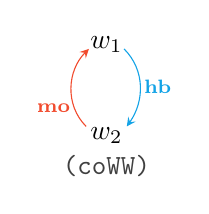
\begin{tikzpicture}[x=1em,y=1em,yscale=-1,xscale=-1]
\tikzstyle{every node}=[font=\normalfont]
\node (w1) {$ w_1 $};
\node (w2) [below=20pt of w1] {$ w_2 $};
\node (coww) [below=-3pt of w2] {\hl{coWW}};

\draw [->,>=stealth,color=Cerulean] ($ (w1.south east)+(.3,-5pt) $) to[out=135,in=-125] node[midway,right=-2pt,font=\scriptsize] {\textcolor{black}{\lhb}} ($ (w2.north east)+(0.2,3pt) $);
\draw [->,>=stealth,color=RedOrange] ($ (w2.north west)+(-0.2,3pt) $) to[out=-45,in=45] node[left=-2pt,pos=.25,font=\scriptsize] {\textcolor{black}{\lmo}}($ (w1.south west)+(-0.3,-5pt) $);

\end{tikzpicture}
} &
			\resizebox{0.25\textwidth}{!}{\tikzset{every picture/.style={line width=0.75pt}} %set default line width to 0.75pt        
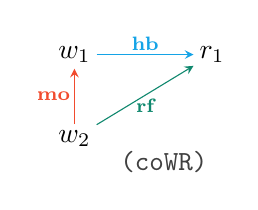
\begin{tikzpicture}[x=1em,y=1em,yscale=-1,xscale=-1]
\tikzstyle{every node}=[font=\normalfont]

\node (w1) [inner sep=2pt] {$ w_1 $};
\node (r1) [right=35pt of w1,inner sep=2pt] {$ r_1 $};
\node (w2) [below=20pt of w1,inner sep=2pt] {$ w_2 $};
\node (cowr) [below right=-4pt and 5pt of w2] {\hl{coWR}};

\draw [->,>=stealth,color=Cerulean] (w1) -- node[midway,above=-2pt,font=\scriptsize,color=black] { $\lhb$ } (r1);
\draw [->,>=stealth,color=PineGreen] (w2) -- node[midway,below=-2pt,font=\scriptsize,color=black]{\lrf} (r1);
\draw [->,>=stealth,color=RedOrange] (w2) -- node[midway,left=-2pt,font=\scriptsize,color=black] { $\lmo$ } (w1);

\end{tikzpicture}
} &
			\resizebox{0.25\textwidth}{!}{\tikzset{every picture/.style={line width=0.75pt}} %set default line width to 0.75pt        
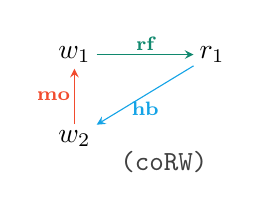
\begin{tikzpicture}[x=1em,y=1em,yscale=-1,xscale=-1]
\tikzstyle{every node}=[font=\normalfont]

\node (w1) [inner sep=2pt] {$ w_1 $};
\node (r1) [right=35pt of w1,inner sep=2pt] {$ r_1 $};
\node (w2) [below=20pt of w1,inner sep=2pt] {$ w_2 $};
\node (corw) [below right=-4pt and 5pt of w2] {\hl{coRW}};

\draw [->,>=stealth,color=Cerulean] (r1) -- node[midway,below=-1pt,font=\scriptsize,color=black] { $\lhb$ } (w2);
\draw [->,>=stealth,color=PineGreen] (w1) -- node[midway,above=-2pt,font=\scriptsize,color=black]{\lrf} (r1);
\draw [->,>=stealth,color=RedOrange] (w2) -- node[midway,left=-2pt,font=\scriptsize,color=black] { $\lmo$ } (w1);

\end{tikzpicture}
} &
			\resizebox{0.27\textwidth}{!}{\tikzset{every picture/.style={line width=0.75pt}} %set default line width to 0.75pt        
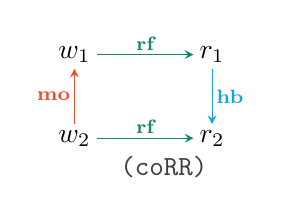
\begin{tikzpicture}[x=1em,y=1em,yscale=-1,xscale=-1]
\tikzstyle{every node}=[font=\normalfont]

\node (w1) [inner sep=2pt] {$ w_1 $};
\node (r1) [right=35pt of w1,inner sep=2pt] {$ r_1 $};
\node (w2) [below=20pt of w1,inner sep=2pt] {$ w_2 $};
\node (r2) [below=20pt of r1,inner sep=2pt] {$ r_2 $};
\node (corr) [below right=-2pt and 5pt of w2] {\hl{coRR}};

\draw [->,>=stealth,color=Cerulean] (r1) -- node[midway,right=-2pt,font=\scriptsize,color=black] { $\lhb$ } (r2);
\draw [->,>=stealth,color=PineGreen] (w1) -- node[midway,above=-2pt,font=\scriptsize,color=black]{\lrf} (r1);
\draw [->,>=stealth,color=PineGreen] (w2) -- node[midway,above=-2pt,font=\scriptsize,color=black]{\lrf} (r2);
\draw [->,>=stealth,color=RedOrange] (w2) -- node[midway,left=-2pt,font=\scriptsize,color=black] { $\lmo$ } (w1);

\end{tikzpicture}
} \\
			\hline
		\end{tabular}
		\label{fig:como}
	\end{figure}
	
	
	\begin{itemize}[label=setmm,align=left,leftmargin=*]
		\item [$\setRF$] The relation is formed from write events 
			to read events, since fences cannot be both, the $\setRF$
			relations remains unchanged \ie $\rf{\imm{\tau}}{}{}$ =
			$\setRF$.
		
		\item [$\setRF^{-1}$] The relation remains unchanged as 
			$\setRF$ remains unchanged \ie $\rfinv{\imm{\tau}}{}{}$ 
			= $\setRF^{-1}$.
		
		\item [$\setMO$] Assume $\exists w, w' \in \events_\tau$ \st 
			as a consequence of synthesizing fences in the buggy trace 
			$\tau$ to form $\imm{\tau}$, $w$ is modification-ordered
			before $w'$. However, $(w,w') \nin \mo{\imm{\tau}}{}{}$
			since we consider $\mo{\imm{\tau}}{}{}$ = $\setMO$.
			
			We show by case analysis on the coherence conditions
			involving $\mo{\imm{\tau}}{}{}$ that \ourtechnique does
			not miss a weak cycle by not expanding modification-order
			after synthesizing fences.
		
			Consider the following coherence conditions involving 
			$\mo{\imm{\tau}}{}{}$:
		
			\begin{itemize}[label=CoWW,align=left,leftmargin=*]
			\item [CoWW:] Let $\exists w_1, w_2 \in \writes$
				\st $\hb{\imm{\tau}}{w_1}{w_2}$. 
			
				If $\mo{\tau}{w_1}{w_2}$ then there does not
				exist a violation.
			
				However, if $\mo{\tau}{w_2}{w_1}$ then we will 
				detect the violation as a cycle in 
				$\mo{\imm{\tau}}{}{};\hb{\imm{\tau}}{}{}$
				(depicted diagrammatically in \hlref{coWW}).
			
			\item [CoWR:] Let $\exists r_1 \in \reads$, 
				$\exists w_1,w_2 \in \writes$ 
				\st $\hb{\imm{\tau}}{w_1}{r_1}$ and 
					$\rf{\imm{\tau}}{w_2}{r_1}$.
			
				If $\mo{\tau}{w_1}{w_2}$ then there does not
				exist a violation.
			
				However, if $\mo{\tau}{w_2}{w_1}$ then we will 
				detect the violation as a cycle in 
				$\mo{\imm{\tau}}{}{};\hb{\imm{\tau}}{}{};\rfinv{\imm{\tau}}{}{}$
				(depicted diagrammatically in \hlref{coWR}).
				
			\item [CoRW:] Let $\exists r_1 \in \reads$, 
				$\exists w_1,w_2 \in \writes$ 
				\st $\rf{\imm{\tau}}{w_1}{r_1}$ and 
				$\hb{\imm{\tau}}{r_1}{w_2}$.
			
				If $\mo{\tau}{w_1}{w_2}$ then there does not
				exist a violation.
			
				However, if $\mo{\tau}{w_2}{w_1}$ then we will 
				detect the violation as a cycle in 
				$\mo{\imm{\tau}}{}{};\rf{\imm{\tau}}{}{};\hb{\imm{\tau}}{}{}$
				(depicted diagrammatically in \hlref{coRW}).
			
			\item [CoRR:] Let $\exists r_1,r_2 \in \reads$,
				$\exists w_1, w_2 \in \writes$
				\st $\rf{\imm{\tau}}{w_1}{r_1}$, 
					$\rf{\imm{\tau}}{w_2}{r_2}$ and
					$\hb{\imm{\tau}}{r_1}{r_2}$. 
					
					If $\mo{\tau}{w_1}{w_2}$ then there does not
					exist a violation.
					
					However, if $\mo{\tau}{w_2}{w_1}$ then we will 
					detect the violation as a cycle in 
					$\mo{\imm{\tau}}{}{};\rf{\imm{\tau}}{}{};\hb{\imm{\tau}}{}{};\rfinv{\imm{\tau}}{}{}$
					(depicted diagrammatically in \hlref{coRR}).
		\end{itemize}
	\end{itemize}

	Thus, \ourtechnique does not miss a cycle in any
	coherence rule and	\wkfence is sound.
\end{proof}

\noindent
\cc defines a total-order on \sc ordered events in agreement with
the $\setHB$, $\setMO$, $\setRF$ relations.
%
We borrow the following definition of total-order from 
\cite{C11}\cite{vafeiadis2015common}:
Given

$order(P,R)$ $\definedas$ 
	($\nexists a\ R(a,a)$) $\^$
	($R^+ \subseteq R$) $\^$
	($R \subseteq P \times P$);  and,

$total(P,R)$ $\ \definedas$
	$\forall a,b\ P(a) \^ P(b)$ $\implies$
	$a = b$ $\v$ $R(a,b)$ $\v$ $R(b,a)$.
\newline
%
All \sc ordered events must form a total order $\setTO$ \st
the following two conditions are satisfied:

\begin{enumerate}
	\item $order(\ordevents{\sc},\setTO)$ $\^$ 
		$total(\ordevents{\sc},\setTO)$ $\^$ $\onsc{\setHB}$ 
		$\intersection$ $\onsc{\setMO}$ $\subseteq$ $\setTO$
		\hfill [coTO]
	\item $\forall \rf{\tau}{e_w}{e_r}$ \st $e_r \in 
		\ordevents{\sc}_\tau$
		\begin{itemize}
			\item either, $e_w \in \ordevents{\sc}_\tau$ $\^$ 
				$\to{\tau}{e_w}{e_r}$ $\^$ $\nexists e_w' 
				\in \ordevents{\sc}_\tau$ \st 
				$\to{\tau}{\to{\tau}{e_w}{e_w'}}{e_r}$,
				\hfill [rfTO1]
			\item or, $e_w \nin \ordevents{\sc}_\tau$ $\^$
				$\nexists e_w' \in \ordwrites{\sc}_\tau$ \st
				$\hb{\tau}{e_w}{e_w'}$ $\^$ 
				($\to{\tau}{e_w'}{e_r}$ \st $\nexists e_w'' \in$
				$\ordwrites{\sc}$ where
				$\to{\tau}{\to{\tau}{e_w'}{e_w''}}{e_r}$).
				\hfill [rfTO2]
		\end{itemize}
	\item  $\forall \rf{\tau}{e_w}{e_r}$ \st $e_w \in 
		\ordevents{\sc}_\tau$, $\exists \mathbb{F} \in
		\ordfences{\sc}_\tau$ \st $\seqb{\tau}{\mathbb{F}}{e_r}$
		$\^$ $\to{\tau}{e_w}{\mathbb{F}}$
		$\^$ $\nexists e_w' \in \ordwrites{\sc}$ where
		$\to{\tau}{\to{\tau}{e_w}{e_w'}}{\mathbb{F}}$.
		\hfill [FrfTO]
\end{enumerate}

\noindent
Recall that, the relation $\setSO$ has been defined in 
Section~\ref{sec:invalidating ce} as follows:\newline
	$\forall e_1, e_2 \in \events_\tau$ \st 
	$(e_1,e_2) \in$ $\setHB$ $\union$ $\setMO$ $\union$ $\setRF$ 
	$\union$ $\setFR$ 
	
	if
	$e_1, e_2 \in \ordevents{\sc}_\tau$ then 
	$\so{\tau'}{e_1}{e_2}$; \hfill[so1]
	
	if
	$e_1 \in \ordevents{\sc}_\tau$, 
	$\exists \mathbb{F}^\sc \in \ordsfences{\sc}_{\tau'}$ where
	$\seqb{\tau'}{e_2}{\mathbb{F}^\sc}$ then
	$\so{\tau'}{e_1}{\mathbb{F}^\sc}$;
	\hfill[so2]
	
	if
	$e_2 \in \ordevents{\sc}_\tau$, 
	$\exists \mathbb{F}^\sc \in \ordsfences{\sc}_{\tau'}$ where
	$\seqb{\tau'}{\mathbb{F}^\sc}{e_1}$ then
	$\so{\tau'}{\mathbb{F}^\sc}{e_2}$;
	\hfill[so3]
	
	if
	$\exists \mathbb{F}^\sc_1$, $\mathbb{F}^\sc_2$ 
	$\in \ordsfences{\sc}_{\tau'}$ where
	$\seqb{\tau'}{\mathbb{F}^\sc_1}{e_1}$ and 
	$\seqb{\tau'}{e_2}{\mathbb{F}^\sc_2}$ then
	$\so{\tau'}{\mathbb{F}^\sc_1}{\mathbb{F}^\sc_1}$.
	\hfill[so4]


{\lemma {$\setSO \subseteq \setTO$ ($\setSO$ does not relate 
		two events that are not related by rules for $\setTO$)}
	\label{lem:so subset to}}
\begin{proof}
		By definition of $\setSO$, $\so{\tau}{e^\sc_1}{e^\sc_2}$ if
		\begin{itemize}[label=so4,align=left,leftmargin=*]
			\item [so1:] $e^\sc_1, e^\sc_2 \in \ordevents{\sc}_\tau$
				and $(e^\sc_1, e^\sc_2) \in$ $\setHB$ $\union$ 
				$\setMO$ $\union$ $\setRF$ $\union$ $\setFR$
				
				$\implies$ $\to{\tau}{e^\sc_1}{e^\sc_2}$
				(using [coTO] and [rfTO1]).
				
			\item [so2:] $e^\sc_1 \in \ordevents{\sc}_\tau$,
				$e^\sc_2 \in \ordfences{\sc}_\tau$
				and $(e^\sc_1, e^\sc_2) \in$ ($\setHB$ $\union$ 
				$\setMO$ $\union$ $\setRF$ $\union$ $\setFR$);$\setSB$
			
				$\implies$ $\to{\tau}{e^\sc_1}{e^\sc_2}$
				(using [coTO] and \hlref{coherence conditions} 
				since $\setSB$ $\subseteq$ $\setHB$).
				
			\item [so3:] $e^\sc_2 \in \ordevents{\sc}_\tau$,
				$e^\sc_1 \in \ordfences{\sc}_\tau$
				and $(e^\sc_1, e^\sc_2) \in$ $\setSB$;($\setHB$ 
				$\union$ $\setMO$ $\union$ $\setRF$ $\union$ $\setFR$)
			
				$\implies$ $\to{\tau}{e^\sc_1}{e^\sc_2}$
				(using [to] since $\setSB$ $\subseteq$ $\setHB$).
				
			\item [so2:] $e^\sc_1, e^\sc_2 \in \ordfences{\sc}_\tau$
				and $(e^\sc_1, e^\sc_2) \in$ $\setSB$;($\setHB$ $\union$ 
				$\setMO$ $\union$ $\setRF$ $\union$ $\setFR$);$\setSB$
			
				$\implies$ $\to{\tau}{e^\sc_1}{e^\sc_2}$
				(using [to] since $\setSB$ $\subseteq$ $\setHB$).
		\end{itemize}
\end{proof}


{\lemma {\stfence is sound: if there does not exist a total order on
	the \sc ordered events of a trace $\tau$ then there exists a cycle 
	in $\setSO$.} \label{lem:strong-sound}}
\begin{proof}
	Consider $e^\sc_1, e^\sc_2 \in \ordevents{\sc}_\tau$ \st 
	both $\to{\tau}{e^\sc_1}{e^\sc_2}$ and 
	$\to{\tau}{e^\sc_2}{e^\sc_1}$ agree with the other event relations.
	To form the total order we can assume either one of the two orders
	\cite{C11}. Assume $\to{\tau}{e^\sc_1}{e^\sc_2}$.
	
	Further, consider a total order cannot be formed on \sc events of
	the intermediate trace $\imm{\tau}$ \st
	$\to{\imm{\tau}}{e}{\to{\imm{\tau}}{...}{\to{\imm{\tau}}{e^\sc_1}{\to{\imm{\tau}}{e^\sc_2}{\to{\imm{\tau}}{...}{e}}}}}$
	then we simply reverse to $\to{\imm{\tau}}{e^\sc_2}{e^\sc_1}$ and
	eliminate the cycle.
	
	Thus, pairs of \sc ordered events that don't have a fixed order
	cannot contribute to a strong cycle. \hfill{\it inf}(i).
	
	Given $e^\sc_1, e^\sc_2 \in \ordevents{\sc}_{\imm{\tau}}$
	$\to{\imm{\tau}}{e^\sc_1}{e^\sc_2}$ if 
	\begin{itemize}[label=to2,align=left,leftmargin=*]
		\item [to1:] $(e^\sc_1, e^\sc_2) \in$ $\setHB$ $\union$ 
			$\setMO$ $\union$ $\setRF$ $\union$ $\setFR$
		
			$\implies$ $\so{\imm{\tau}}{e^\sc_1}{e^\sc_2}$
			(using [so1]).
			
			Thus, such events are related by $\so{\imm{\tau}}{}{}$
			and would be considered by finding strong cycles.
		
		\item [to2:] $e^\sc_1$ $R_1;R_2;...;R_n$ $e^\sc_2$, where 
			$R_i \in \{\setHB, \setMO, \setRF, \setFR\}$.
			
			It may be the case that $\nso{\imm{\tau}}{e^\sc_1}{e^\sc_2}$
			because [so2], [so3] and [so4] only cover a subset of such 
			cases. However, if
			\begin{enumerate}
				\item if $e^\sc_1 \neq e^\sc_2$ then there is no cycle;
				\item if $e^\sc_1 = e^\sc_2$ then the cycle violates a
					coherence condition and a corresponding weak cycle
					would be detected.
			\end{enumerate}
	\end{itemize}
	Thus, cycles created due to [to2] are not strong cycles and
	$\so{\imm{\tau}}{}{}$ relates events related by $\to{\imm{\tau}}{}{}$
	using [to1].\hfill{\it inf}(ii).
	
	Thus, from {\it inf}(i) and (ii) and Lemma~\ref{lem:so subset to}, 
	\stfence is sound.
\end{proof}

{\lemma {{\tt AssignMO} is sound: \ourtechnique does not assign a memory
	order to a fence that is too weak to stop the buggy trace.}
	\label{lem:mo-sound}}
\begin{proof}
	By definition of \hlref{coherence conditions} if there exists
	a weak cycle in the intermediate trace $\imm{\tau}$ then 
	$\exists$ $\sw{\imm{\tau}}{e}{e'}$ $\v$ 
	$\dob{\imm{\tau}}{e}{e'}$. 
	
	Since, the buggy trace $\tau$ was returned by the counter
	example generators 
	
	$\implies$ $\neg\sw{\tau}{e}{e'}$ $\^$
	$\neg\dob{\tau}{e}{e'}$
	
	$\implies$ either $e$ or $e'$ or both are candidate fences 
	introduced by \ourtechnique.
	
	By definitions of $\sw{\imm{\tau}}{e}{e'}$ and 
	$\dob{\imm{\tau}}{e}{e'}$
	if $e$ is a fence then its memory order must be \rel or 
	stricter, if $e'$ is a fence then its memory order must be 
	\acq or stronger.
	
	Thus, the locally assigned memory orders are sufficiently 
	strong.\hfill{\it inf}(i)\newline
	
	\noindent
	If there exists a fence, $\mathbb{F}$,  that was locally 
	assigned a memory order $m$ and after coalescing with other 
	buggy trace the final memory order of $\mathbb{F}$ is $m'$
	then either $m' = m$ or $m'$ is stronger than $m$
	(by construction).
	
	\noindent
	Since from {\it inf}(i) we know that $m$ was sufficiently 
	strong then final memory order $m'$ is also sufficiently strong. 
	
\end{proof}

{\theorem {\ourtechnique is sound: If a buggy trace can be stopped 
		by synthesizing \cc fences and \ourtechnique stops the trace.}}
\begin{proof}
	Consider induction on the number of buggy traces. 
	Let {\tt CE} represent the set of counter examples or buggy traces.
	
	\noindent
	{\sl Base Case:} Consider $|${\tt CE}$|$ = 1. 
	Using Lemma~\ref{lem:weak-sound} and Lemma~\ref{lem:strong-sound}
	we can state that a violation in \hlref{coherence conditions} or
	\sc total order is not missed by \ourtechnique. \newline
	%	
	Further the fences introduced for at least 1 of the violations
	exist in the final solution (by construction of SAT query).
	\newline
	%
	Hence, \ourtechnique is sound for 1 trace.\newline
	
	\noindent 
	{\sl Induction Hypothesis:}
	Assume that \ourtechnique is sound for $|${\tt CE}$|$ = N.
	\newline
	
	\noindent
	{\sl Induction Step:}
	Consider $|${\tt CE}$|$ = N+1.
	
	Since, we take a conjunction on the SAT formulas from various
	traces thus at least 1 cycle from each trace exists in the 
	{\tt min-model} (by construction of SAT query).\newline
	%
	Further, we know from Lemma~\ref{lem:mo-sound} that \ourtechnique
	assigns memory orders that can stop all the corresponding traces.
	\newline
	%
	Thus, \ourtechnique is sound for N+1 buggy traces.
\end{proof}

{\lemma {{\tt min-model} returns the optimal number of fences.}
	\label{lem:opt-num}}
\begin{proof}
	Let $\mathcal{F}$ represent the set of fences returned by
	{\tt min-model} and let $\mathcal{F}^o$ represent the optimal set
	of fences. Assume $|\mathcal{F}^o| < |\mathcal{F}|$.
	
	The min-model of the non-optimal solution is computed using a
	SAT solver (\z) and the computation is assumed to be correct. 
	As the consequence,
	$|\mathcal{F}^o| < |\mathcal{F}|$ $\implies$ the optimal result
	was not a part of the SAT query formula.
	
	Using Lemma~\ref{lem:weak-sound} and 
	Lemma~\ref{lem:strong-sound} we know that \ourtechnique does 
	not miss any weak or strong cycle
	$\implies$ every set of fences that forms a correct solution,
	including the optimal solution, is contained in the SAT query
	formula.
	
	Thus, by contradiction, $|\mathcal{F}| = |\mathcal{F}|^o$ 
	\ie {\tt min-model} returns the optimal number of fences.
\end{proof}

{\theorem {\ourtechnique synthesizes the optimal number of fences
	with the optimal memory orders.}}
\begin{proof}
	Let {\tt min-cycles} represent the set of weak and strong 
	cycles of all buggy traces \st every candidate fence in the 
	cycle belongs to {\tt min$\Phi$}. 
	
	We know that {\tt AssignMO} iterates over cycles in {\tt 
	min-cycles} and takes union over fences of cycles from 
	{\tt min-cycles}. As {\tt min$\Phi$} consists of the optimal
	number of fences (Lemma~\ref{lem:opt-num}) then union over
	cycles of {\tt min-cycles} has the same set of fences as
	{\tt min$\Phi$}.\newline
	Thus, \ourtechnique is optimal in the number of fences.
	\newline
	
	Consider induction on the number of counter examples or buggy
	traces {\tt CE}.\newline
	
	\noindent
	{\sl Base Case-1:} Consider $|${\tt CE}$|$ = 1.
	By definition of {\tt AssignMO} each fence is locally assigned
	the weakest memory order that is sound (Lemma~\ref{lem:mo-sound}).

	Thus, \ourtechnique is optimal in the memory order of fences
	for 1 buggy trace.
	\newline
	
	\noindent
	{\sl Base Case-2:} Consider $|${\tt CE}$|$ = 2.
	Let $\tau_1c_i$ for $i \in \{1...M_1\}$ represent the $M_1$
	cycles of trace $\tau_1$ and 
	let $\tau_2c_j$ for $j \in \{1...M_2\}$ represent the $M_2$
	cycles of trace $\tau_2$.
	Further, let $\tau_1c_i-\tau_2c_j$ represent the coalesce of 
	cycles $\tau_1c_i$ and $\tau_2c_j$.
	
	Each coalesced solutions has the same number of fences = 
	fences of {\tt min$\Phi$} because {\tt min$\Phi$} returns the
	minimum number of fences required to stop $\tau_1$ and $\tau_2$.
	
	\noindent
	If $\exists \mathbb{F}$ fence with memory order $m$ in a 
	cycle $\tau_1c_i$ but the final solution of \ourtechnique
	assigns memory order $m'$ to $\mathbb{F}$ \st $m'$ is stronger
	than $m$
	
	then, $\exists \tau_2c_j$ where memory order of $\mathbb{F}$ is
	$m'$ (by construction of coalesced solutions),
	
	further, $\nexists \tau_2c_k$ where memory order of $\mathbb{F}$
	is $m$ \st $score(\tau_1c_i-\tau_2c_k) < score(\tau_1c_i-\tau_2c_j)$
	(where $score(x)$ represents the score of the solution $x$).
	
	Thus, \ourtechnique is optimal in the memory order of fences
	for 2 buggy traces.
	\newline 
	
	\noindent
	{\sl Induction Hypothesis:} Assume, \ourtechnique is optimal in the 
	memory order of fences for N buggy trace.
	\newline
	
	\noindent
	{\sl Induction Step:} 
	Consider $|${\tt CE}$|$ = N+1.
	Let $s_1, ..., s_M$ represent the $M$ coalesced solutions for 
	buggy traces $\tau_1, ..., \tau_N$ and $\tau_{N+1}c_i$ for 
	$i \in \{1, ..., P \}$ represent the $P$ cycles of $(N+1)^{th}$
	trace.
	
	Every coalesced solution $\tau_{N+1}s_j$ has the same number of 
	fences = fences of {\tt min$\Phi$} because {\tt min$\Phi$} 
	returns the minimum number of fences required to stop 
	$\tau_1, ..., \tau_{N+1}$.
	
	If $\exists \mathbb{F}$ fence with memory order $m$ in a 
	cycle $\tau_{N+1}c_i$ but the final solution of \ourtechnique
	assigns memory order $m'$ to $\mathbb{F}$ \st $m'$ is stronger
	than $m$
	
	then, $\exists s_j$ where memory order of $\mathbb{F}$ is
	$m'$ (by construction of coalesced solutions),
	
	further, $\nexists s_k$ where memory order of $\mathbb{F}$
	is $m$ \st $score(\tau_{N+1}c_i-s_k) < score(\tau_{N+1}c_i-s_j)$
	(where $score(x)$ represents the score of the solution $x$).
	
	Thus, \ourtechnique is optimal in the memory order of fences
	for N+1 buggy traces.
\end{proof}

\end{document}
